\chapter{Анализ свойств метода оценки синхронизации с нулевым фазовым сдвигом.}~\label{chapt3}
В этой главе мы исследуем свойства методов, основанных на проекции от протечки сигнала,
а также сравним результаты их работы с методами, являющимися на данный
момент стандартом в области исследований функциональной коннективности.

Начнем с исследования свойств базовой процедуры, описанной в разделе~\ref{sec:psiicos}.
\section{Исследование воспроизводимости решения для метода PSIICOS.}\label{sec:bootstrap}

Для проверки стабильности решений мы использовали процедуру бутстрэпа, аналогичную
описанной в~\cite{Darvas2005}.
Мы генерировали $B$ различных кросс-спектральных временных рядов (CT), полученных
усреднением по эпохам, индексы которых берутся как сочетания с повторениями, набранные
с равными вероятностями из полного набора индексов.

Затем на каждой итерации бутстрэпа небольшое
число пар $m$, соответствующих сетям с наибольшими
значениями кросс-спектральных коэффициентов, полученными в результате применения
алгоритма PSIICOS, группировались в несколько кластеров в соответствии с процедурой
попарной пространственной кластеризации (Pairwise Spatial Clustering,~\cite{Zalesky2012}).

Для каждого полученного кластера мы рассчитывали среднюю сеть. Для этого мы усредняли
координаты начал и концов сетей в кластере, предварительно ориентируя их таким
образом, чтобы концы были направлены в одну полуплоскость.
Средние сети, полученных на каждом шаге бутстрэпа, сохранялись.

Для количественной оценки пространственного разброса полученных таким образом средних сетей
мы определяли расстояние между парой сетей как минимум по двум возможным ориентациям
сетей от суммы евклидовых расстояний между их концами.

В соответствии с определенной таким образом функцией расстояния мы определяли индекс
воспроизводимости $\eta$ как единицу, деленную на среднее по всем $B$ средним сетям расстояние
от сети до ближайшего соседа.

\section{Симуляции методом Монте-Карло.}\label{sec:monte_carlo_simulation}
Чтобы сравнить предложенный алгоритм с другими методами, оценивающими коннективность
в пространстве источников, мы сконструировали ряд реалистичных симуляций.

Для симуляций использовали поверхность коры реального испытуемого,
реконструированную по МРТ-снимкам при помощи пакета программ Freesurfer.
Для аппроксимации этой поверхности трехмерной вычислительной сеткой мы
использовали 15000 узлов. Для этой поверхности мы рассчитали матрицу прямой модели
высокого разрешения $\matr{G}^{HR}$, в которой на каждую точку коры приходится
две топографии, соответствующие модели со свободной ориентацией диполя для МЭГ
в случае сферической симметрии. Эти топографии мы рассчитывали при помощи метода главных
компонент для $M \times 3$ прямой модели для отдельно взятой точки, выкидывая
компоненту с наименьшим собственным числом.

Мы симулировали 100 повторений (эпох) эксперимента, в котором за стимулом следовал
всплеск индуцированной активности на частоте 10 Гц. Индуцированная активность
симулировалась как пары синусоид, не привязанные по фазе к стимулу, но с неслучайной
разностью фаз по отношению друг к другу. Их разность фаз $\delta\phi$ выбиралась
для каждой эпохи случайно из равномерного распределения на отрезке $[-\pi/4, \pi/4]$.

Шум мозга мы моделировали как $Q=1000$ кортикальных источников, активность которых
никак не связана со стимулом. Положения на коре этих источников
выбирались для каждой эпохи независимо и случайно.

Для моделирования их временных профилей активации мы фильтровали реализации гауссовского
случайного процесса полосовым БИХ-фильтром пятого порядка в полосах частот,
соответствующих тета (4--7 Гц), альфа (8--12 Гц), бета (15--30 Гц) и гамма (30--50, 50--70 Гц)
активности. Относительные вклады этих полос частот мы взвешивали таким образом, чтобы
итоговая спектральная плотность мощности имела вид $1/f$, соответствующий реалистичному
спектру данных МЭГ. Далее общий вклад шума мозга в итоговый сигнал взвешивался,
чтобы соответствовать типичным соотношениям сигнал-шум, наблюдаемым в реальных
записях.

Для отображения шумовых источников на сенсоры умножали каждый срез полученных временных
профилей на соответствующие столбцы матрицы $\matr{G}^{HR}$ и складывали результаты.

ОСШ в симуляционных данных мы определяли как отношение фробениусовских
норм матрицы данных и матрицы шума, отфильтрованных в целевой полосе (8--12 Гц).

Для вычисления матрицы кросс-спектральной плотности на сенсорах, соответствующей целевой полосе,
мы проводили следующую процедуру.
Мы фильтровали симулированный сигнал на каждом сенсоре в диапазоне (8--12 Гц) и
вычисляли аналитический сигнал.
Затем для каждого временного среза мы брали внешние произведения с сопряжением
комплекснозначного вектора аналитических сигналов на сенсорах и усредняли их по эпохам.

Чтобы наши симуляции были больше приближены к реальным условиям, когда настоящие источники
не всегда точно ложатся на узлы вычислительной сетки, мы использовали сетку с высоким
разрешением (15000 узлов) только для симуляции данных. Для оценки
коннективности по симуляционным данным мы использовали в 10 раз более разреженную сетку,
насчитывающую 1503 узла.

В качестве метрик качества мы использовали кривые Receiver Operating Characteristics (ROC)
и Precision-Recall (PR). Метрика Precision-Recall лучше работает в ситуации, когда
число истинно положительных мало по сравнению с общим количеством вариантов.
ROC-кривая, или график \emph{чувствительность~--- 1 - специфичность} в этом случае информативна
только для очень высоких значений специфичности.

Для каждой реализации метода Монте-Карло мы считали ROC-кривую и затем
усредняли кривые по ансамблю из 1000 реализаций. Сравнения проводились для двух различных
значений ОСШ: 1 и 0.2.

Так как целевой характеристикой предложенного метода является одинаковое качество
решений для произвольных фазовых задержек между связанными источниками, мы сравнивали
поведение методов для двух различных фазовых задержек $\delta\phi=\pi/2-\pi/20$ и
$\delta\phi=\pi/20$ радиан. Также мы исследовали поведение нашего метода на
равномерной сетке средних значений фазового сдвига.

Для первого теста мы моделировали одну пару взаимодействующих источников. Для каждой эпохи
узлы этой сети мы располагали в двух случайно выбранных точках на сетке с высоким разрешением.
Для оценки изменяемой временной активности таких сетей на каждой эпохе мы умножали временной
профиль активации на временное окно, соответствующее активации в течение первой половины
каждой эпохи. % TODO: add ref to picture with window.

На каждой итерации процедуры Монте-Карло мы симулировали данные из 100 эпох с фиксированной
пространственной конфигурацией целевых источников и изменяющейся от эпохи к эпохе конфигурацией
источников шума мозга. Для локализации сетей мы использовали всю протяженность эпохи
чтобы смоделировать ситуацию, когда мы не знаем точно, на каком временном промежутке
сеть активна.

 \begin{figure}[!ht]
 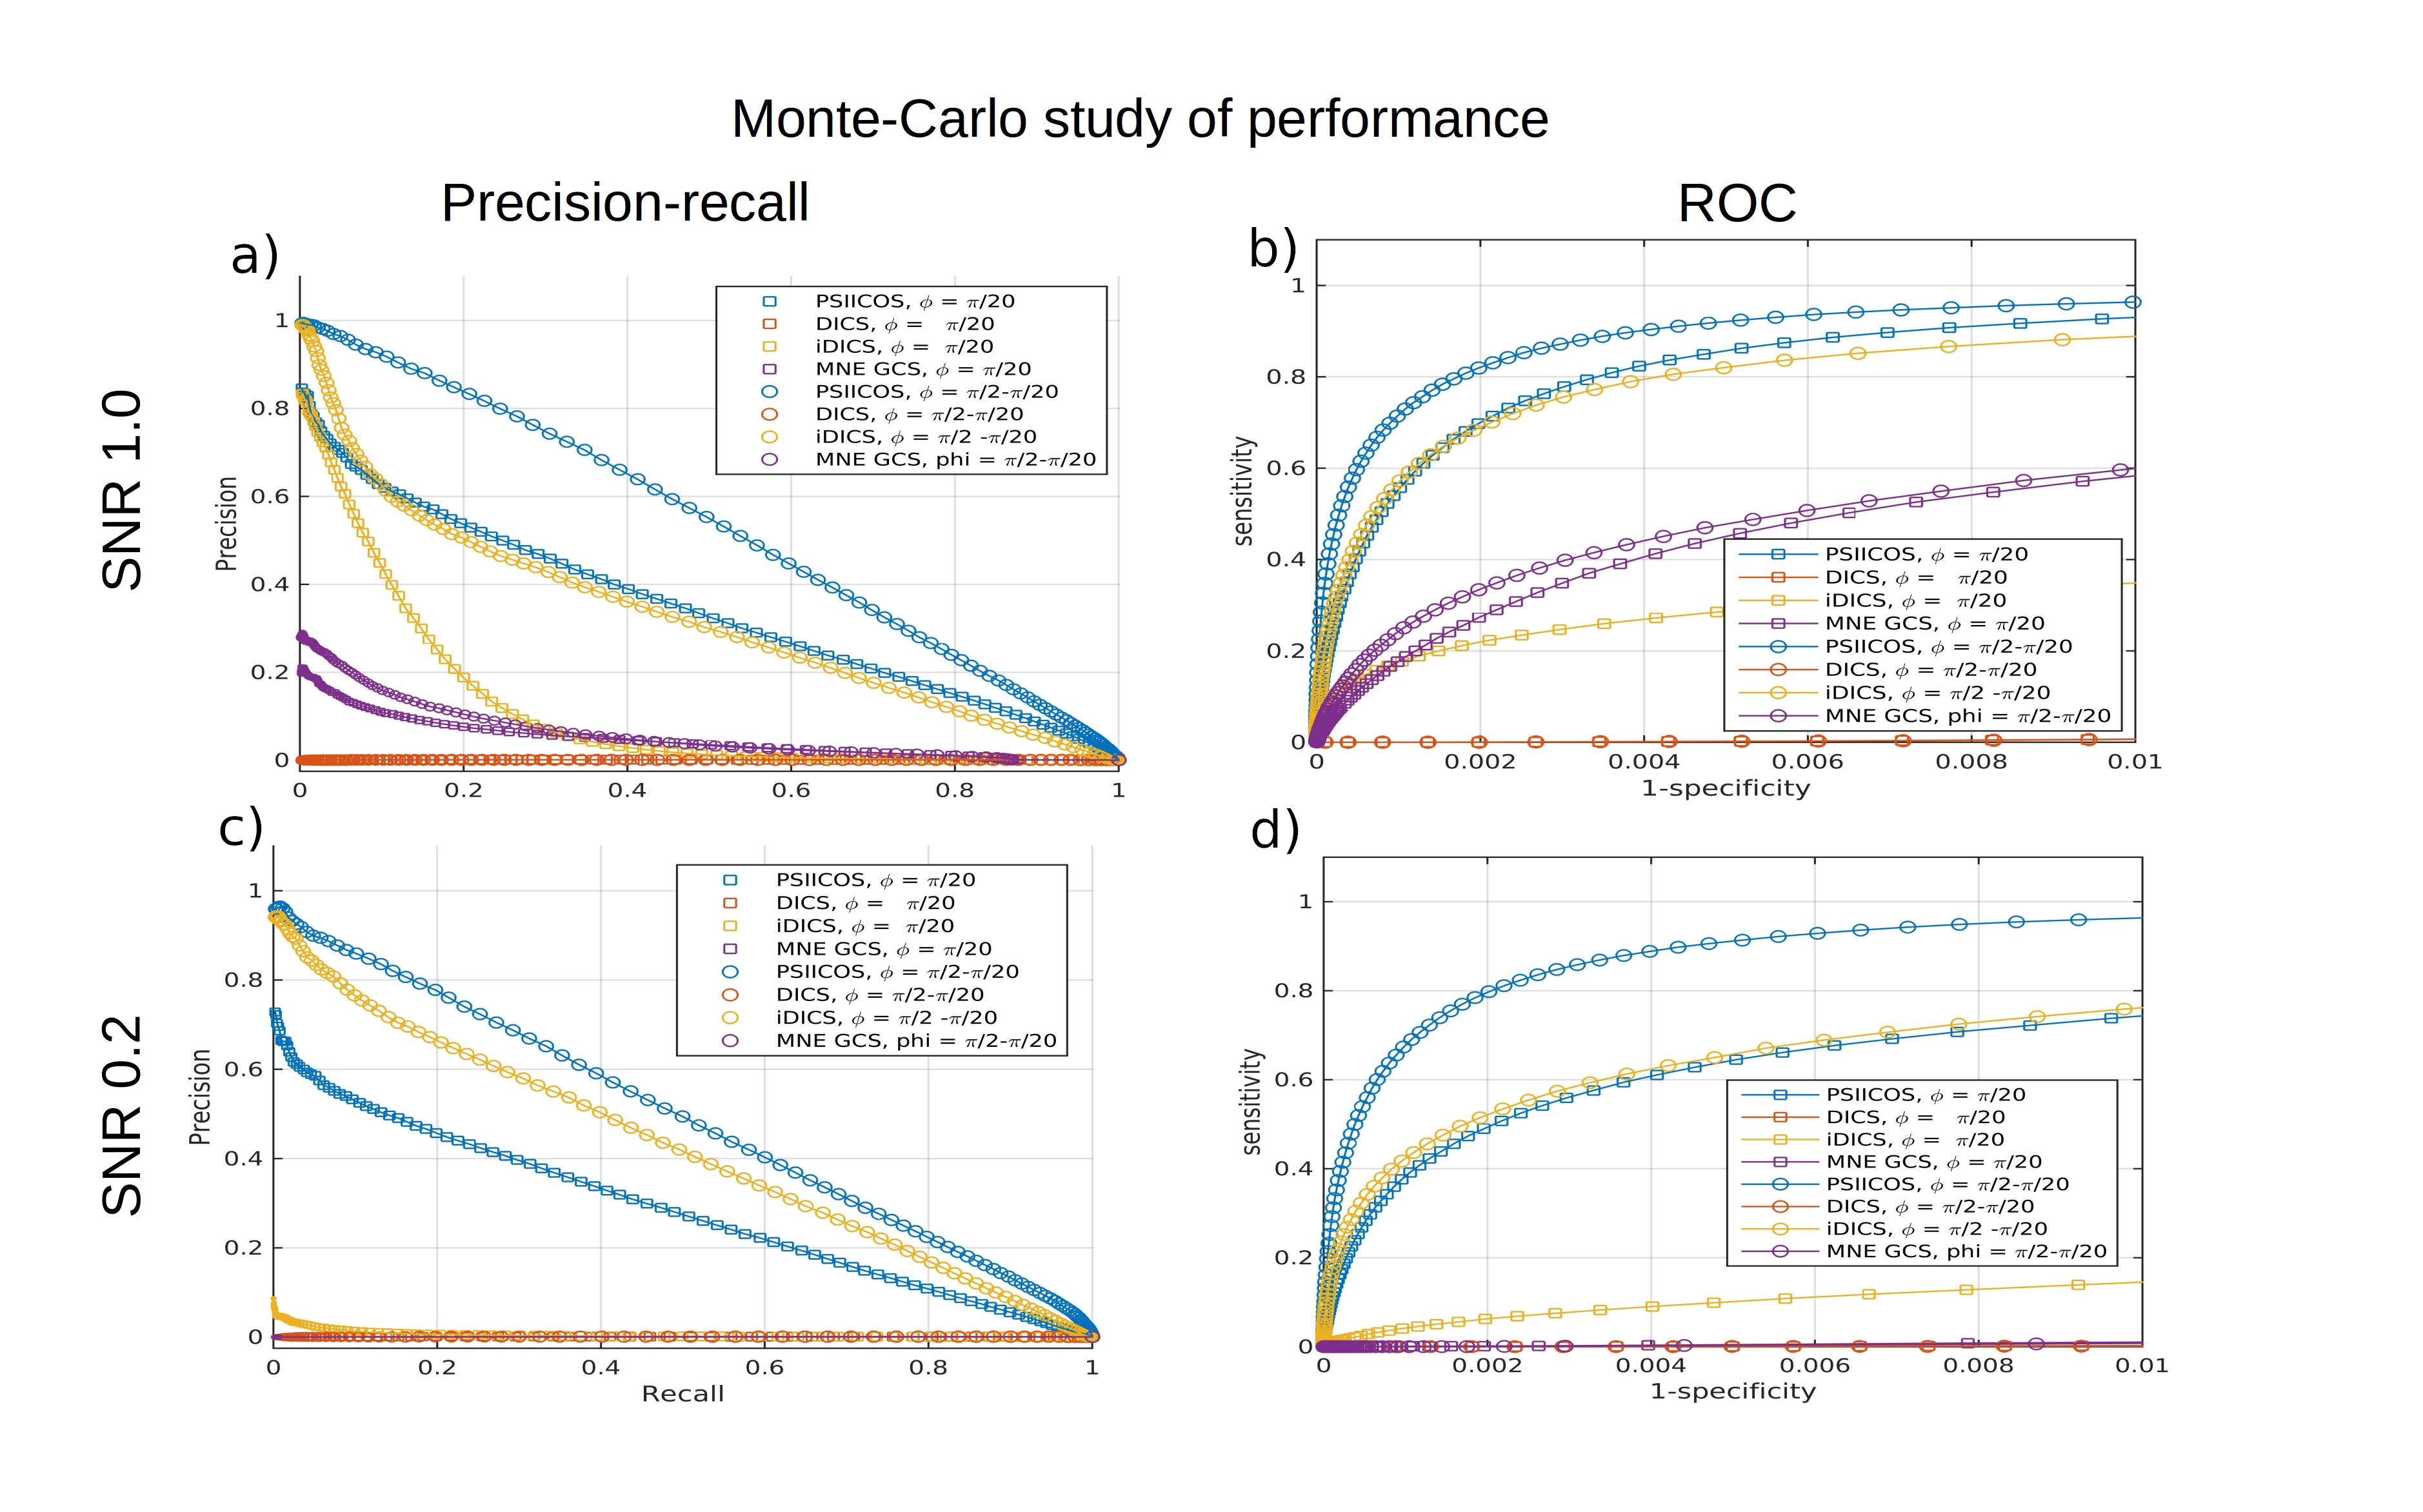
\includegraphics[width=1\textwidth]{../images/psiicos_paper/Figure4_hr_labelled_pans.jpg}
 \caption{Сравнение Precision-Recall (панели (a), (c))  и ROC- (панели (b), (d)) кривых
     в задаче локализации сетей для методов PSIICOS, DICS, iDICS и GCS MNE для
     двух значений ОСШ на основе 1000 Монте-Карло итераций.}\label{fig:04} %Figure 4
\end{figure}%

На графике~\ref{fig:04} видно, что для каждого из условий симуляции качество решений
алгоритма PSIICOS стабильно превосходит другие методы и позволяет получать решения хорошего
качества независимо от величины фазовой задержки.

По графику ROC-кривой для средней разницы фаз $\delta\phi=\pi/2 - \pi/20$ видно, что
показатели iDICS сравнимы с показателями PSIICOS.\@Однако для $\delta\phi = \pi/20$ iDICS
не способен адекватно распознавать сети в силу значительного снижения ОСШ, вызванного
тем, что сети с близкой к нулю фазовой задержкой дают очень маленький вклад во
мнимую часть кросс-спектра.

Метод MNE GCS ведет себя лучше, чем DICS для высоких значений ОСШ. Для низкого ОСШ
оба метода показывают плохие результаты. В то же время метод PSIICOS демонстрирует
адекватное качество решения для обоих значений ОСШ.

В случае низкого ОСШ большая разница в качестве решения PSIICOS между двумя
значениями фазовых задержек вероятно объясняется наличием в итерациях
Монте-Карло сетей с пространственно близкими узлами. Это приводит к тому, что
действительная часть членов, соответствующих истинному взаимодействию,
значительно искажается проекцией. Вместе с тем, остальные методы при таких
условиях для практически перестают работать в случае близких к нулю фазовых задержек.

\section{Симуляции с тремя сетями, перекрывающимися во времени.}\label{sec:three_ntw}
Для второго теста мы симулировали данные с тремя одновременно активными сетями, пространственная
и временная структура активации которых изображены на~\ref{fig:02}.
Главная сложность в этом тесте заключалась в том, чтобы разделить эти три сети в условиях
перекрывающихся окон временной активации.

\begin{figure}[htbp]
    \begin{subfigure}[t]{0.5\textwidth}
        \centering
        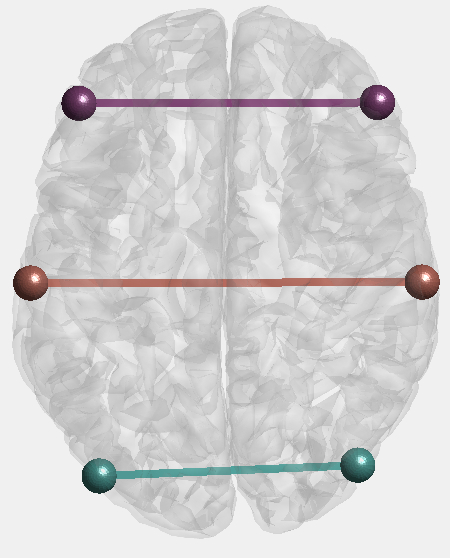
\includegraphics[angle = 90, height = 6cm]{../images/psiicos_paper/Figure2a_hr.jpg}\label{fig:2a}
        \caption{}
    \end{subfigure}
    \begin{subfigure}[t]{0.5\textwidth}
        \centering
        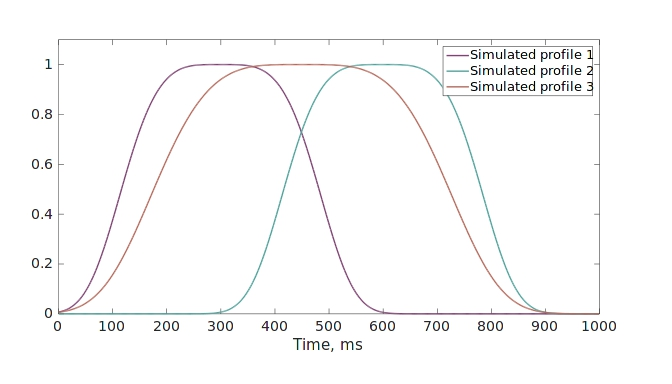
\includegraphics[width=1\textwidth]{../images/psiicos_paper/Figure2b_hr.jpg}\label{fig:2b}
        \caption{}
    \end{subfigure}
    \caption{Три симулированные пары взаимодействующих источников.}\label{02}
        (а)~--- пространственное распределение симулированных источников,
        (б)~--- временные профили активации для каждой из трех сетей.
\end{figure}


Для этих тестов мы сравнивали PSIICOS с тремя другими методами обнаружения
синхронных источников. Первым из этих методов был метод DICS
(см.~\ref{subsec:DICS},~\cite{Gross2001}).  При этом мы восстанавливали
элементы кросс-спектра на источниках, не нормируя их на мощность, чтобы
корректно сравнить результаты с PSIICOS.\@

Чтобы исключить влияние протечки сигнала, мы также использовали
модифицированную версию алгоритма DICS, в которой используется только мнимая
часть кросс-спектра (iDICS, см. разд.~\ref{subsec:iDICS}). Алгоритм iDICS был
вторым из набора методов, с которыми мы сравнивали PSIICOS.\@

В качестве третьего метода мы взяли алгоритм GCS~\ref{subsec:GCS}.  Как и в
оригинальной статье~\cite{Wens2015}, для построения обратного оператора мы
использовали метод MNE~\ref{subsubsec:MNE} и использовали известную матрицу
ковариации шума мозга. Алгоритму PSIICOS эта информация не нужна и поэтому не
использовалась.

На графике~\ref{fig:05} изображена пространственная структура решения для
симуляционных данных в пространстве источников. На графике отображены 0.1\% сетей
с максимальными значениями статистики, оцененной методом PSIICOS и другими тремя
алгоритмами. Как видно из графика, алгоритм PSIICOS сохраняет адекватное качество решения
для всего спектра тестируемых условий.

\begin{figure}[!ht]
 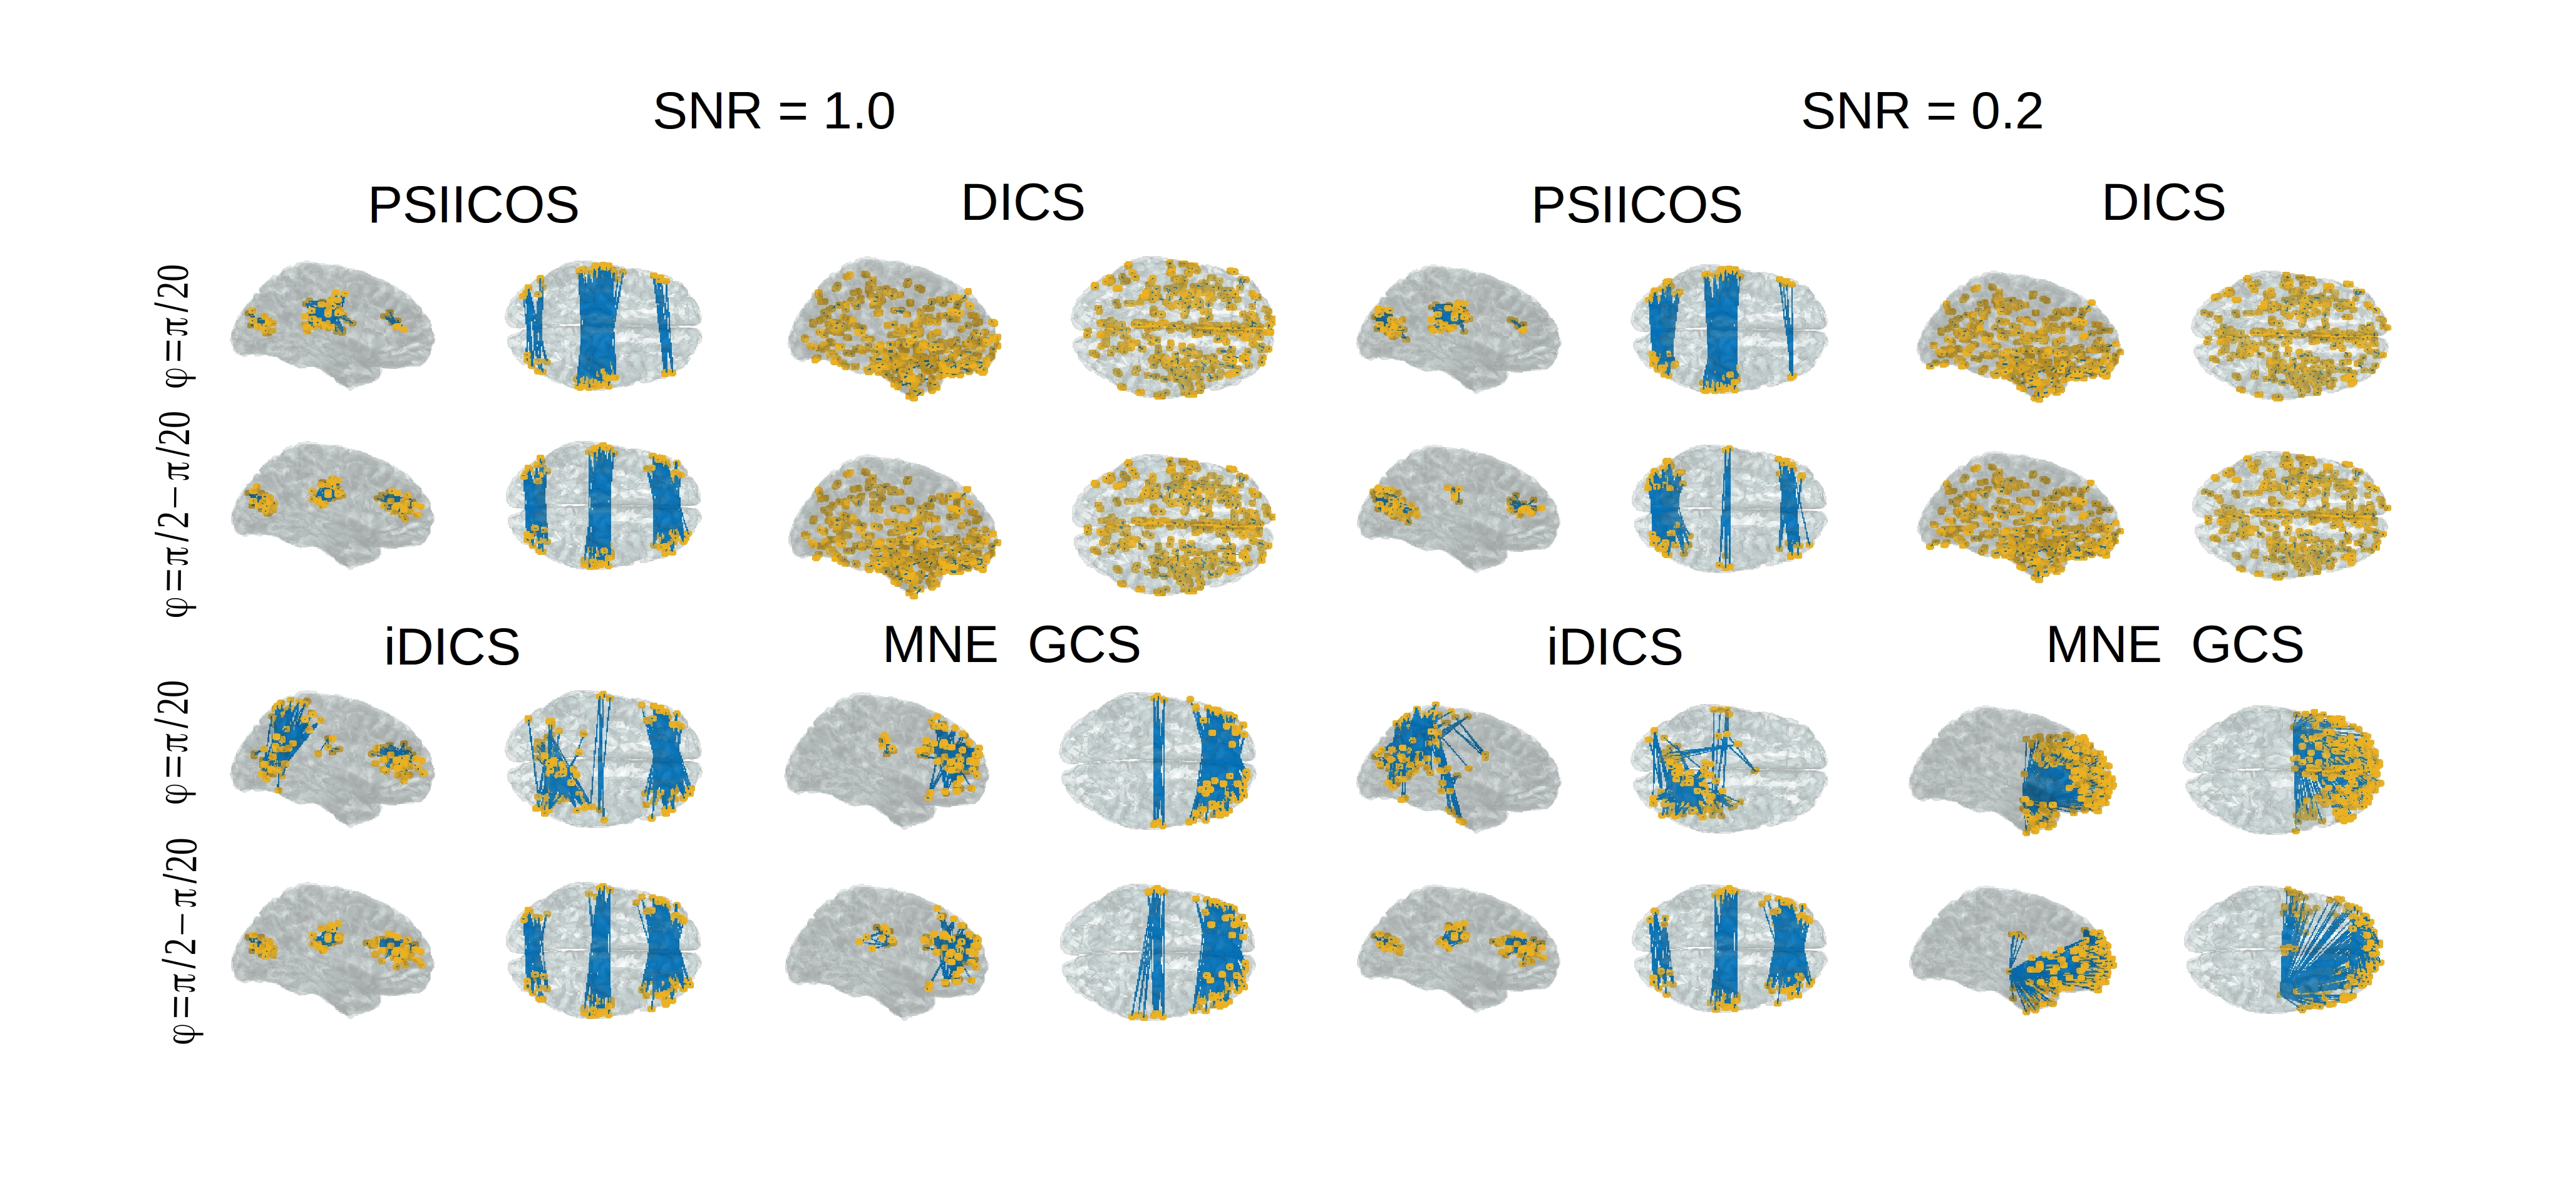
\includegraphics[width=1\textwidth]{../images/psiicos_paper/Figure5_hr.jpg}
 \caption{Пространственное распределение сетевых источников для симуляционных данных.}\label{fig:05} %Figure 5
     На графике изображены 0.1\% сетей с наибольшим значением
     статистики. Из графиков видно, что только алгоритм PSIICOS сохраняет
     качество решения для всего диапазона изучаемых значений.
     Метод iDICS ведет себя практически также хорошо, как и PSIICOS,
     для фазовых сдвигов, близких к $\pi/2$, что согласуется с нашими предыдущими
     результатами. Метод MNE GCS для высоких значений ОСШ достаточно надежно определяет
     две фронтальные сети для каждого значения фазового сдвига, но полностью перестает
     работать для низких значений ОСШ и близких к нулю фазовых задержек. Для задержек,
     близких к $\pi/2$, при низком ОСШ этот метод находит только среднюю сеть
     (для нее индивидуальное ОСШ выше всего) а также порождает большое количество
     ложноположительных срабатываний.
\end{figure}%

Как и для симуляций в разделе~\ref{sec:monte_carlo_simulation}, метод iDICS показывает себя
практически так же хорошо, как и PSIICOS для значений фазовой задержки, близких к $\pi/2$.
Метод MNE GCS для случая высокого ОСШ достаточно надежно определяет две фронтальные сети для
обоих значений фазовой задержки, но полностью перестает работать для низкого ОСШ и
околонулевой разности фаз. Для случая фазовой задержки, близкой к $\pi/2$, и низкого ОСШ
MNE GCS обнаруживает только среднюю сеть (сеть с наибольшим индивидуальным ОСШ) и
порождает большое количество ложно-положительных сетей.

Умножая временной ряд кросс-спектра на сенсорах на среднюю топографию
полученных кластеров, можем восстановить временную активность сетей.
На~\ref{fig:06} изображены временные окна, в течение которых каждая пара
взаимодействующих источников была активна.  Для построения этого графика мы
использовали спроецированный от протечки сигнала временной ряд кросс-спектра,
к которому мы применяли наиболее простую процедуру оценки источников ---
фильтр, максимизирующий SNR в заданной точке~\ref{subsubsec:max_snr_filter}, с
той разницей, что здесь все операции проводились в пространстве 2-топографий с
размерностью $M^2$.

\begin{figure}[!ht]
    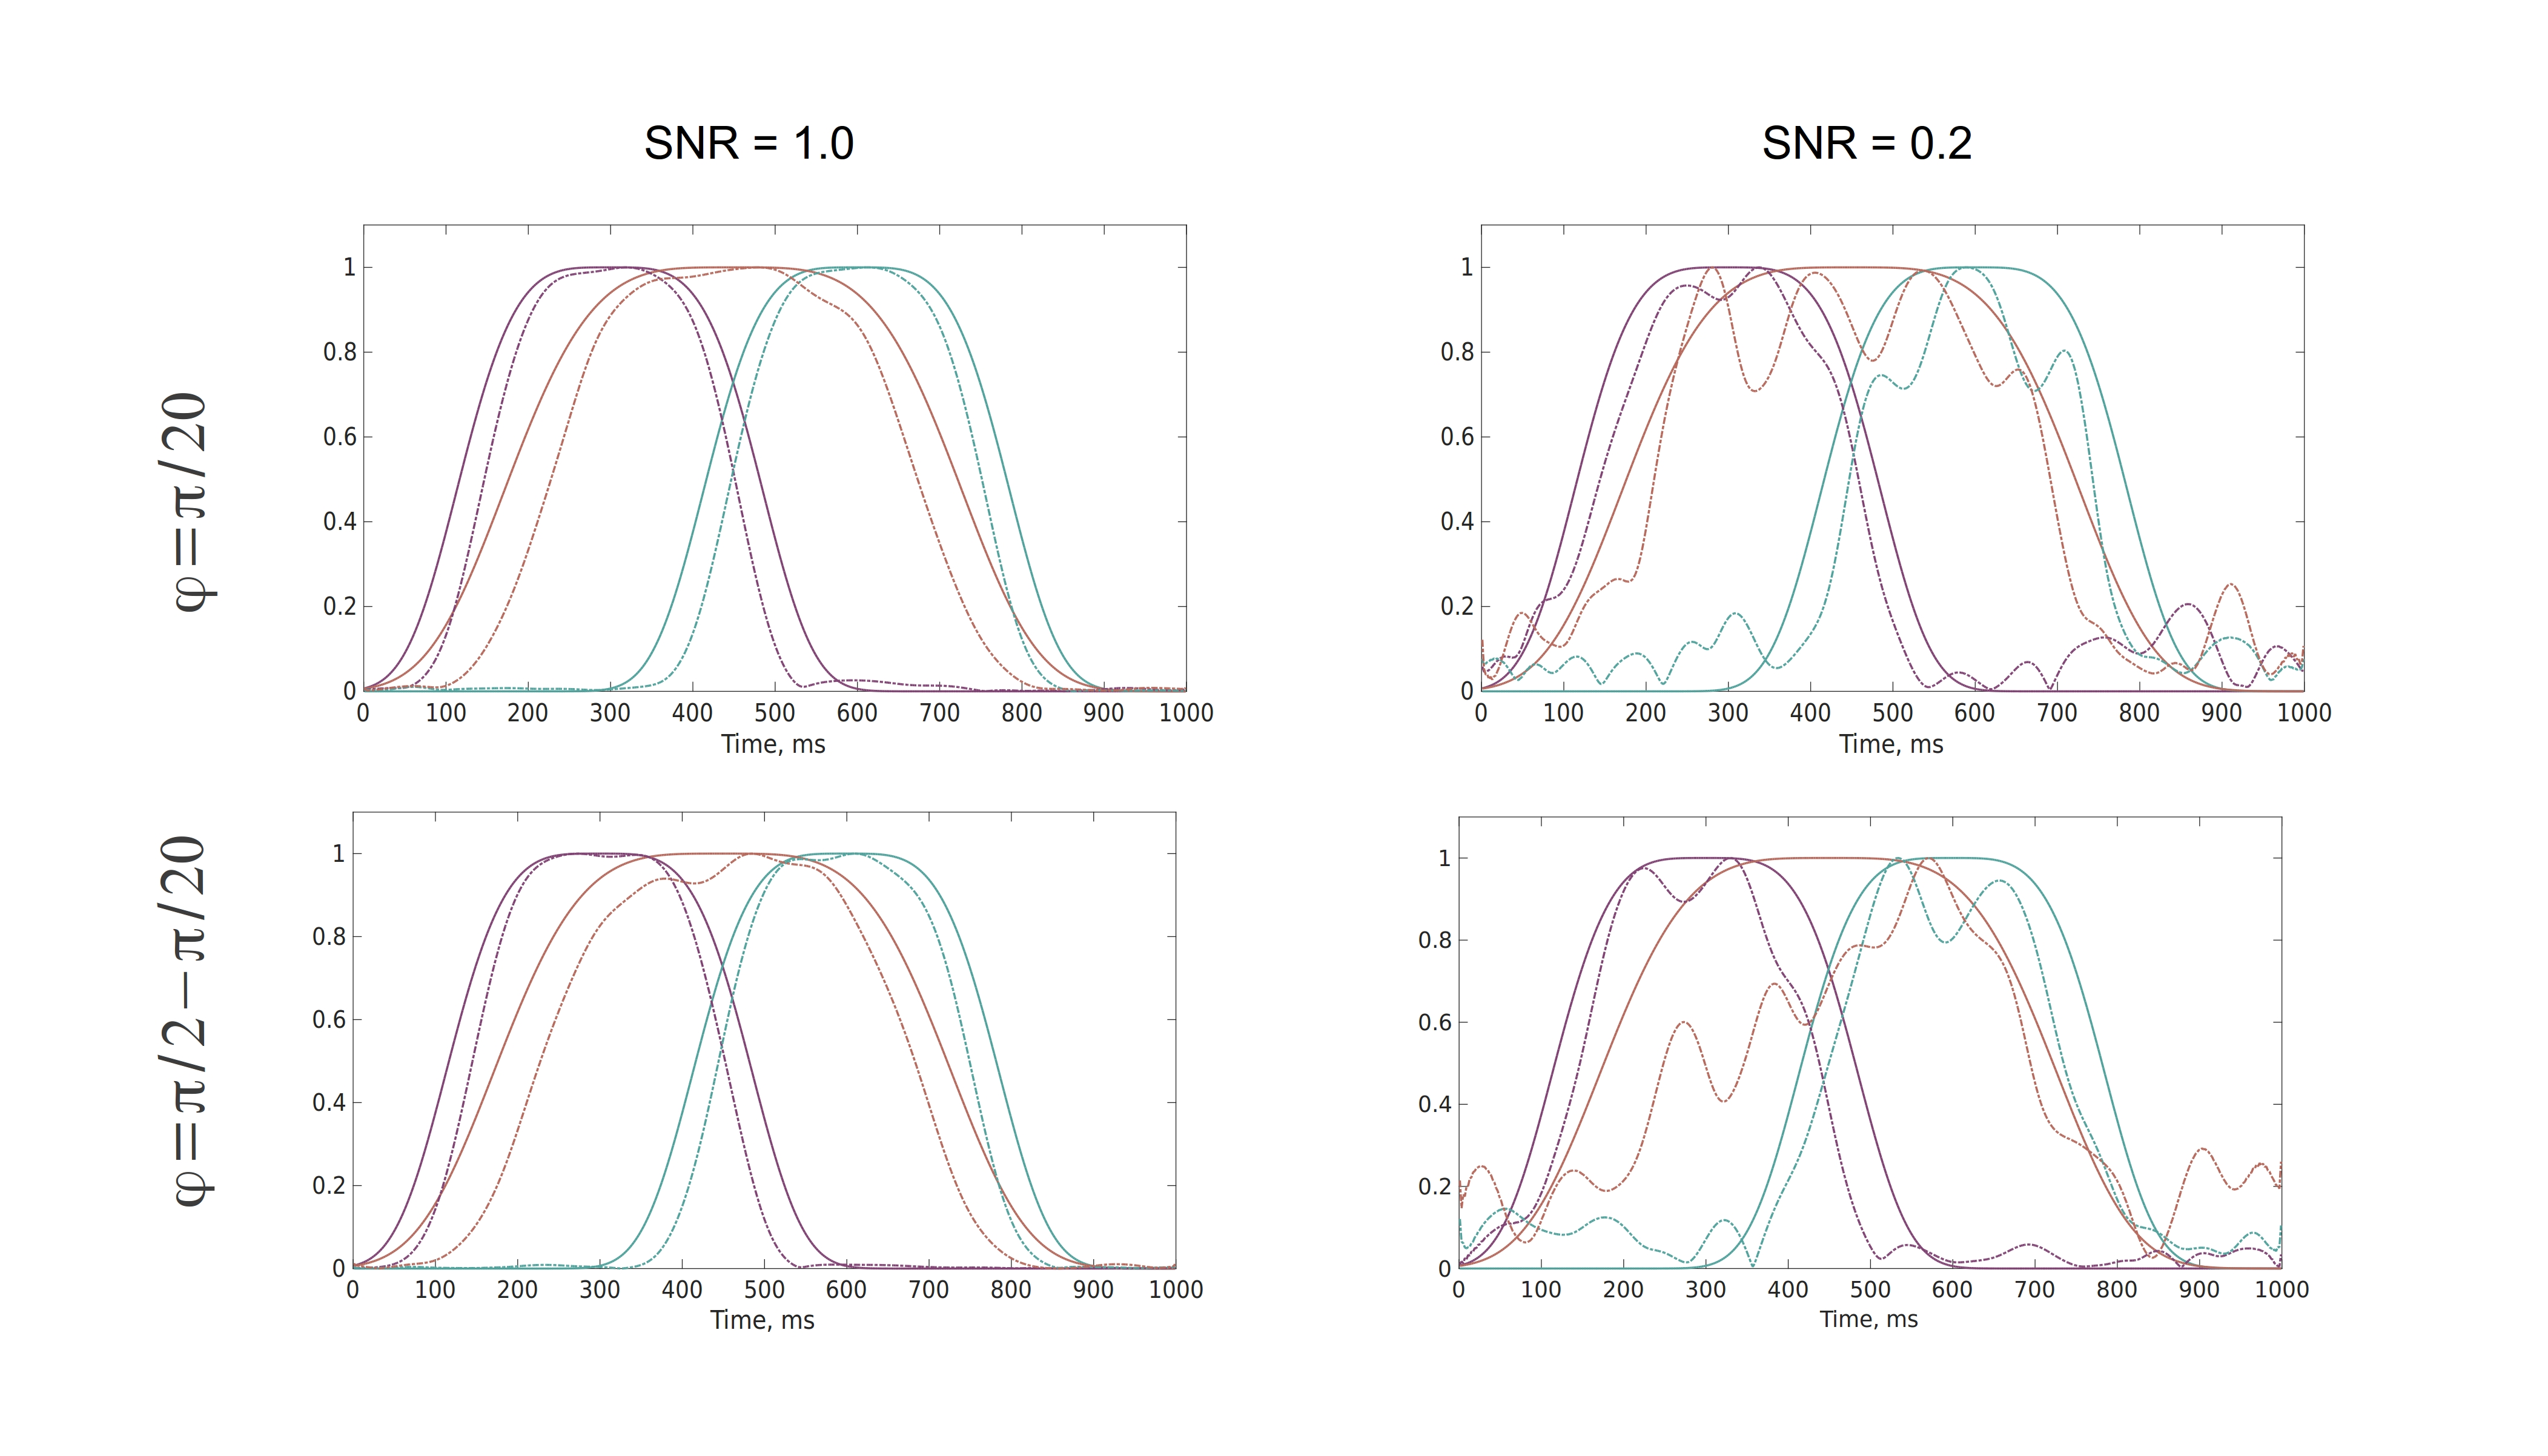
\includegraphics[width=1\textwidth]{../images/psiicos_paper/Figure6_hr.jpg}
    \caption{Временные профили активации симулированных сетей, восстановленные при помощи PSIICOS, для двух
        значений фазового сдвига и двух значений ОСШ.}\label{fig:06} %Figure 6
        Непрерывные линии отображают истинные симулированные профили, а
        пунктир~--- восстановленные алгоритмом PSIICOS.\@
\end{figure}%

Далее, для системного сравнения четырех рассматриваемых методов на графике~\ref{fig:07}
мы модифицированные кривые Precision-Recall, на которых размером маркера мы отобразили
количество истинных сетей, обнаруженных алгоритмом. На левой части рисунка изображен
полный график Precision-Recall; на панелях (b) и (d) показаны данные в диапазоне 0--0.15.

\begin{figure}[!ht]
 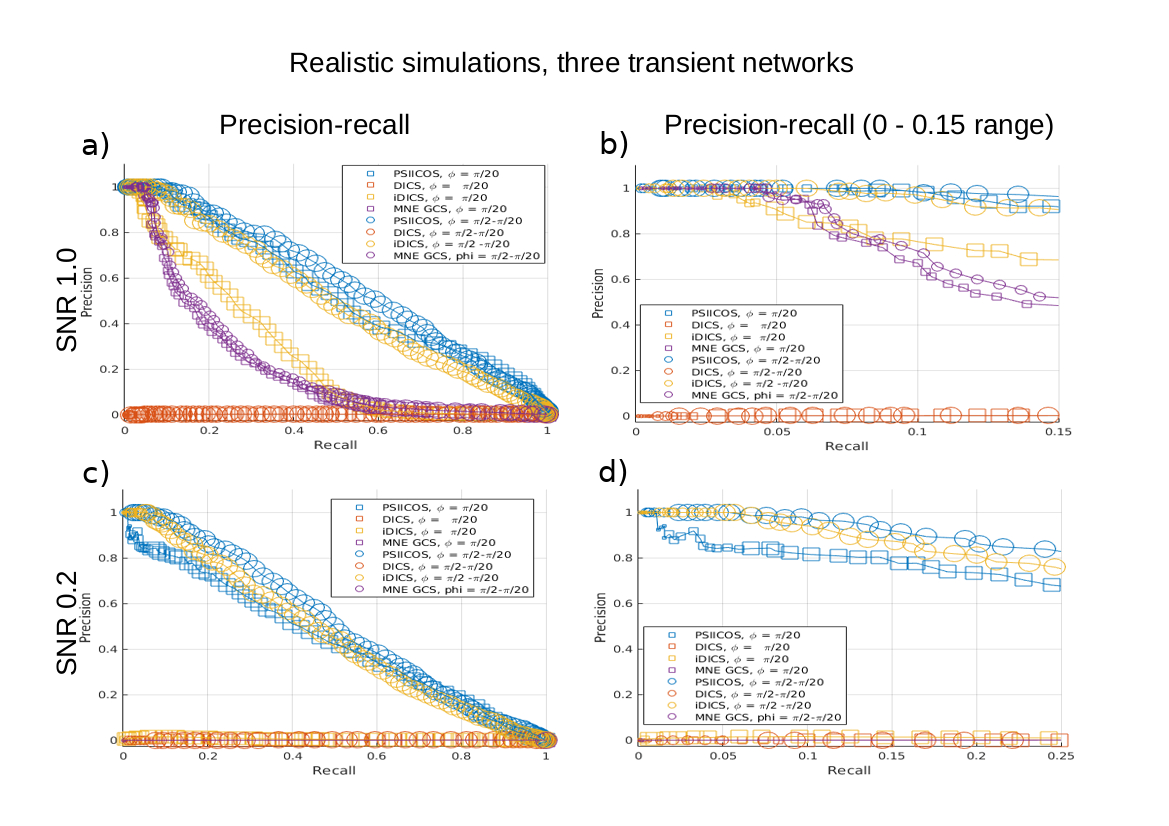
\includegraphics[width=\textwidth]{../images/psiicos_paper/Figure7_hr.jpg}
 \caption{Сравнение PSIICOS с остальными методами в задаче обнаружения трёх
 одновременно активных сетей.}\label{fig:07} %Figure 7
 На рисунках (a), (c) изображены кривые Precision-Recall для всего диапазона
 возможных значений; на рисунках (b), (d) изображены те же кривые, но для
 диапазона значений 0--0.15.
\end{figure}%

Структура этих графиков подтверждает выводы, основанные на визуальном анализе
пространственного распределения обнаруженных сетей (см. рис.~\ref{fig:05}).

Использованные до сих пор метрики оценивают качество решения независимо от порога,
что не годится для оценки качества работы алгоритма на реальных данных.
Для применения к реальным данным мы предлагаем использовать процедуру бутстрэпа,
описанную в разделе~\ref{sec:bootstrap}, чтобы оценить стабильность
получаемых решений и использовать ее в качестве метрики качества.
График~\ref{fig:08} иллюстрирует результаты процедуры
бутстрэпа в применении к реалистичным симуляционным данным.

\begin{figure}[!ht]
 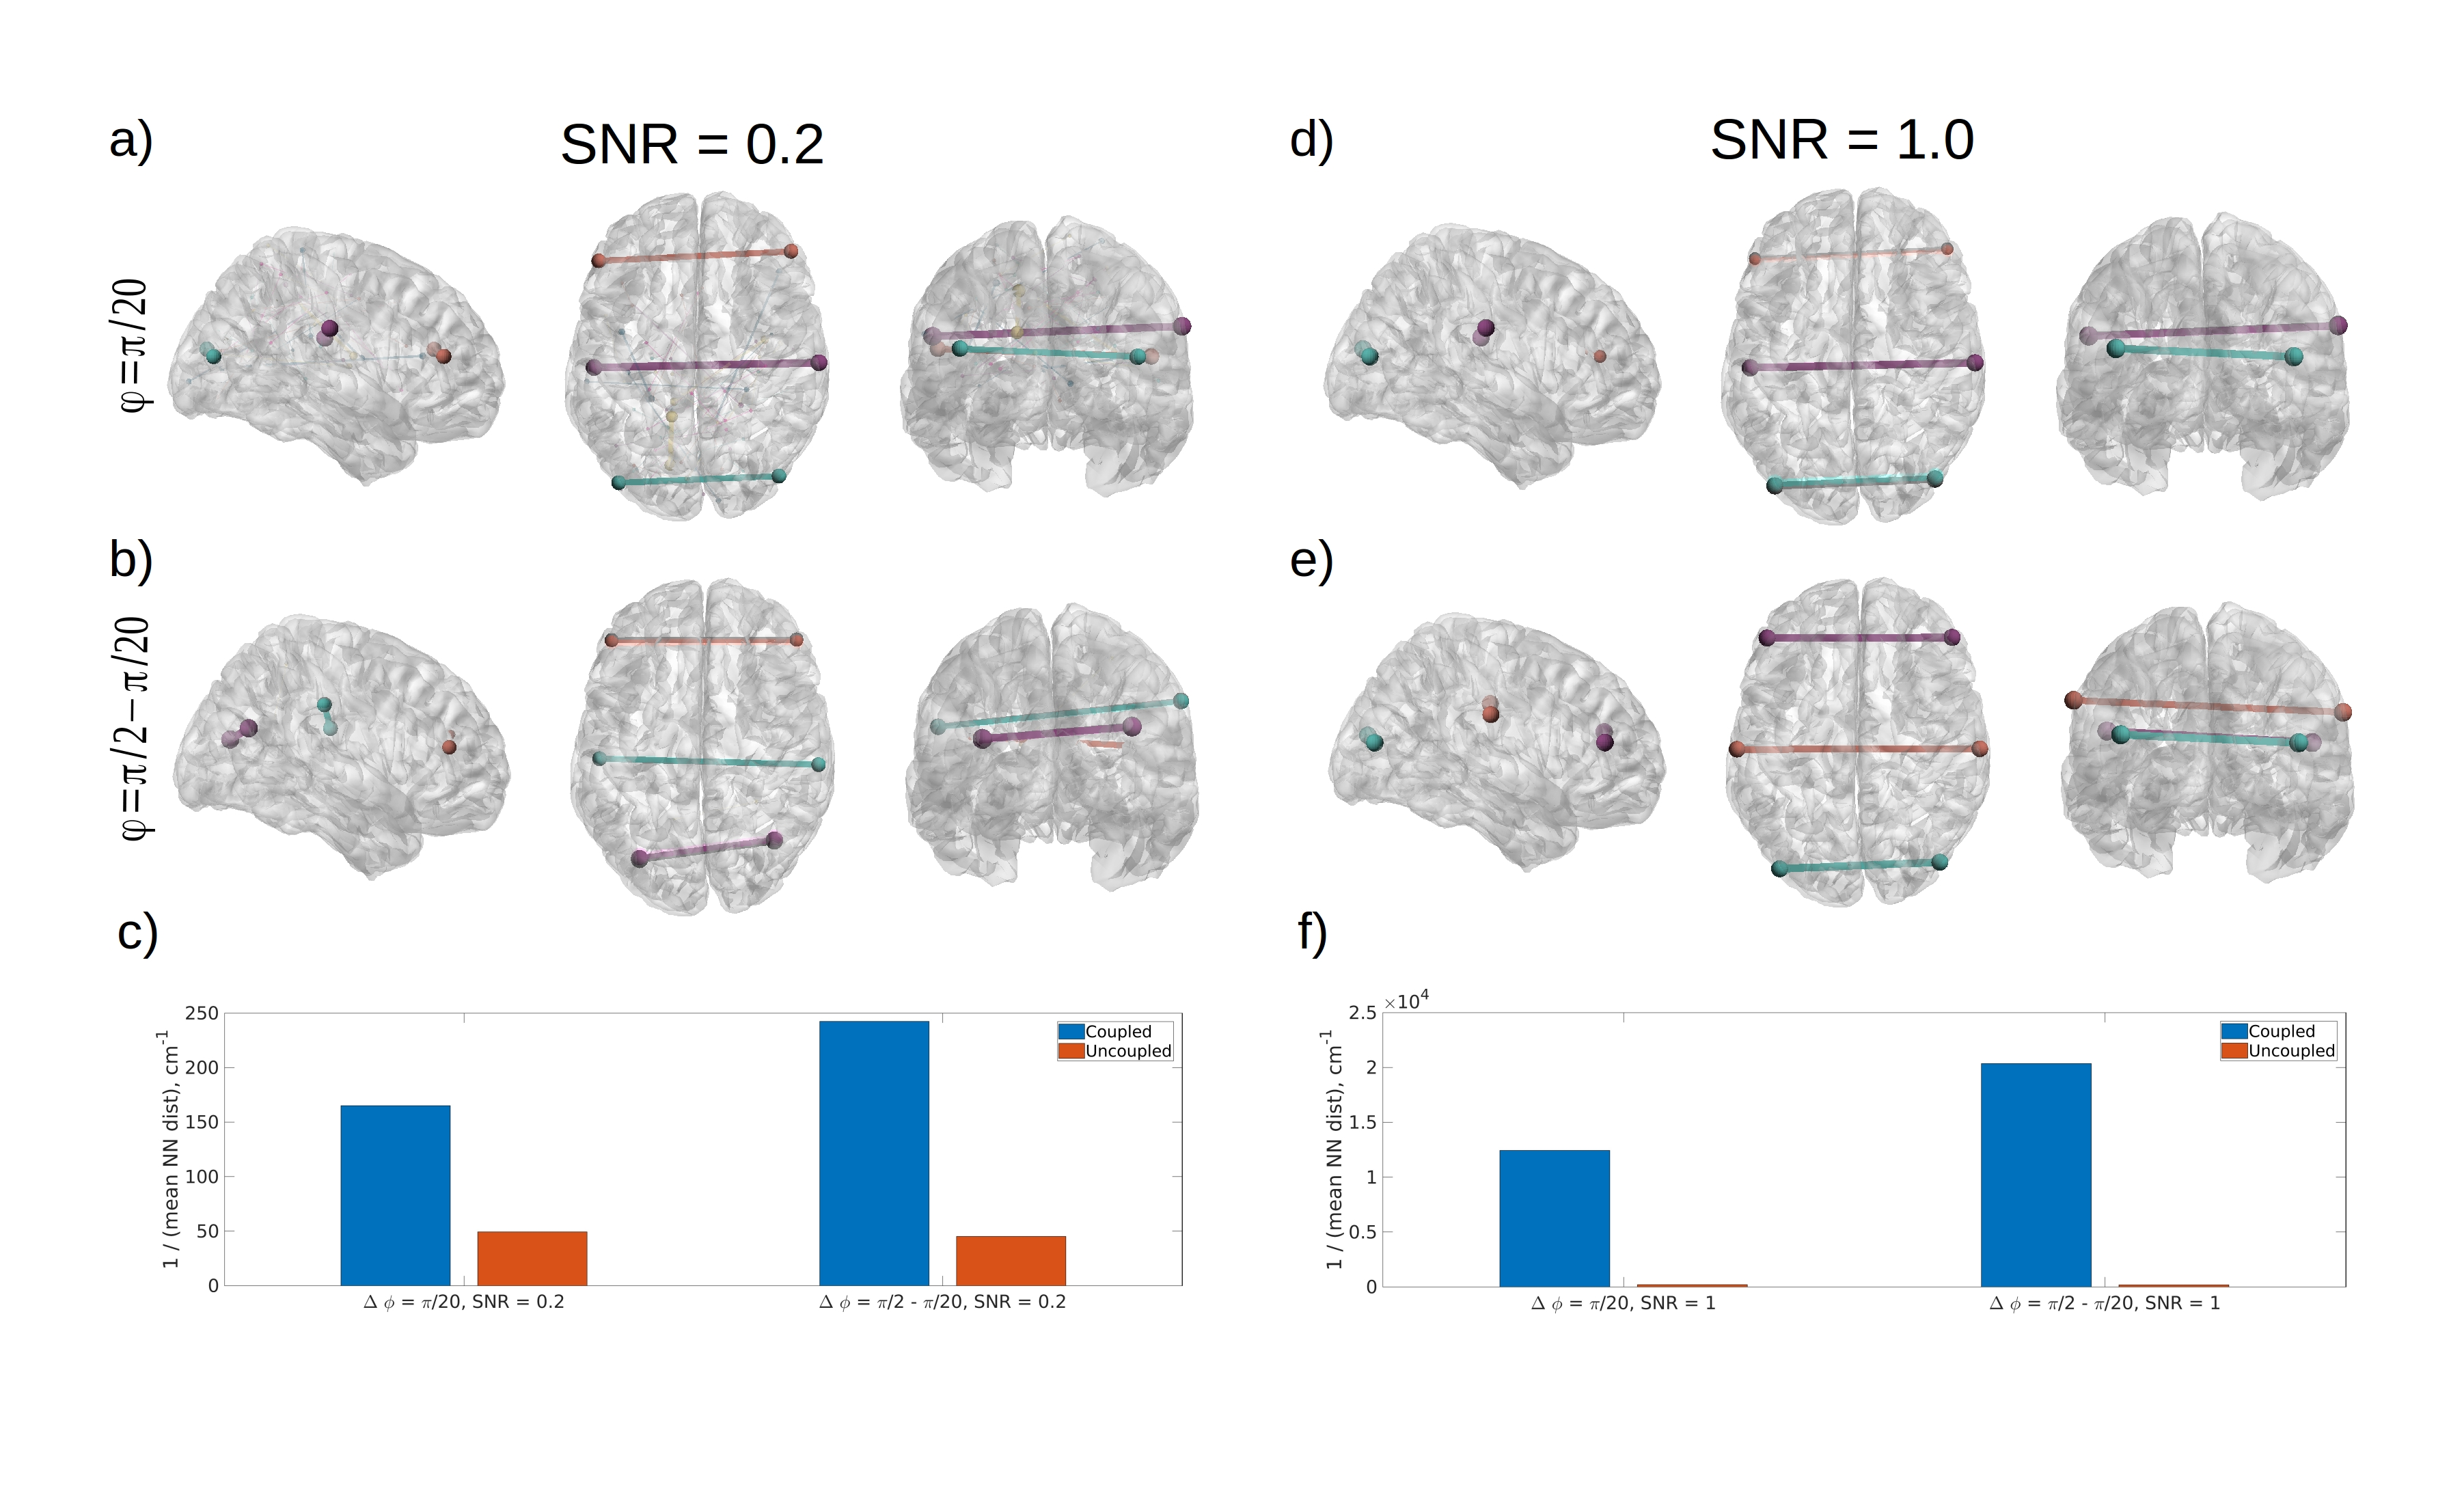
\includegraphics[width=\textwidth]{../images/psiicos_paper/Figure8_hr.jpg}
 \caption{Исследование стабильности метода PSIICOS при помощи процедуры бутстрэпа для
 двух значений фазового сдвига и двух ОСШ.}\label{fig:08}
 (a), (b), (d), (f)~--- стабильные сети отображены в виде отрезков, концы которых
 соответствуют взаимодействующим областям коры. Насыщенность цвета отрезка
 и его концов прямо пропорциональна коэффициенту воспроизводимости $\eta$,
 оцененному при помощи процедуры бутстрэпа. Отрезки, концы которых
 оказывались ближе 1 см друг к другу, мы рисовали одним цветом.
 На графиках (c) и (d) изображен индекс воспроизводимости $\eta$ для
 двух средних фазовых сдвигов, полученных в результате описанной процедуры
 бутстрэпа для двух различных значений ОСШ (ОСШ=0.2 и ОСШ=1 соответственно).
\end{figure}% Figure 8


Наши симуляции показывают, что предложенный подход позволяет достичь лучшего
качества решений при поиске взаимодействующих источников как при околонулевых,
так и при близких к $\pi/2$ фазовых сдвигах. Более того, алгоритм PSIICOS
позволяет обнаруживать сети для всего спектра возможных фазовых задержек. Чтобы
дополнительно проиллюстрировать это качество, мы применили предложенный метод к
симуляционным данным с тремя сетями на равномерной сетке фазовых задержек в
диапазоне от 0 до $\pi/2$. Этот анализ мы провели для двух значений ОСШ и
сравнили три различных подхода: использование только мнимой части (iDICS),
использование только спроецированной действительной части и использование
полной кросс-спектральной матрицы (PSIICOS). На графике~\ref{fig:09}
изображена метрика качества решения в каждом из случаев для различных фазовых
сдвигов.  В качестве метрики мы использовали площадь под кривой
Precision-Recall. Для значений фазы, близких к $\pi/2$, информация о взаимодействующих
источниках содержится в основном во мнимой части кросс-спектра, что легко
заметить из графика~\ref{fig:09}, где использование только мнимой части позволяет достичь
высокого качества решения для близких к $\pi/2$ фазовых сдвигов. Для реалистичного
значения ОСШ=0.1 качество решения резко ухудшается как только значение фазового сдвига
покидает окрестность точки $\pi/2$.

\begin{figure}[!ht]
 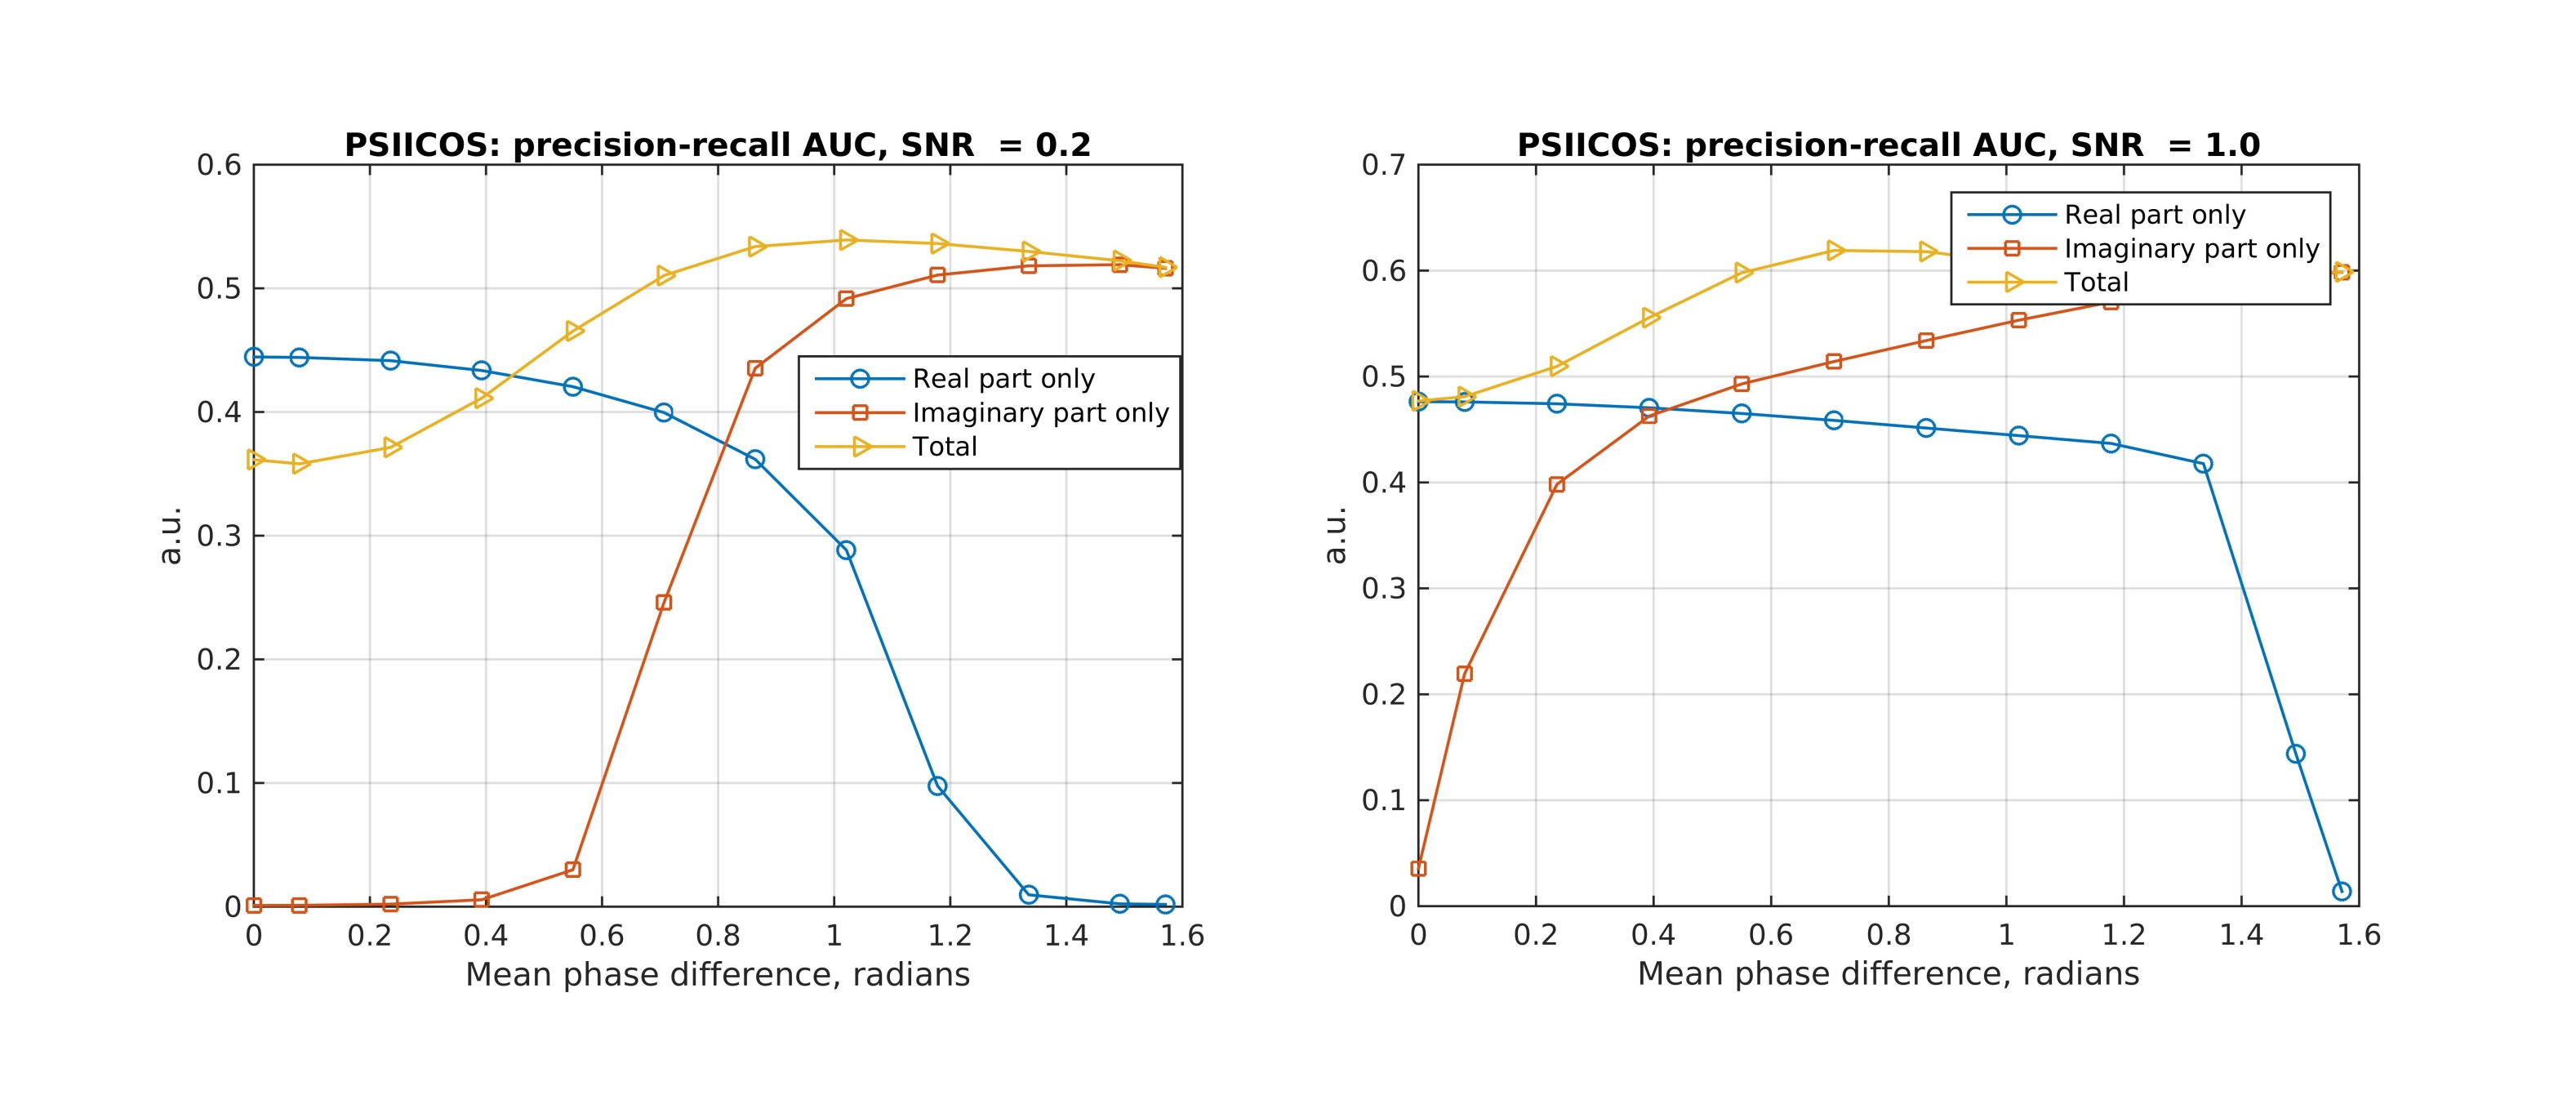
\includegraphics[width=1\textwidth]{../images/psiicos_paper/Figure9_hr.jpg}
 \caption{Качество решений алгоритма PSIICOS как функция средней фазовой задержки}\label{fig:09}
     (a)~--- для низкого значения ОСШ и (b)~--- для высокого.
     Для близких к $\pi/2$ средних значений фазового сдвига информация
     о взаимодействии источников содержится в основном во мнимой части кросс-спектра.
     Поэтому использование только мнимой части (что эквивалентно iDICS) позволяет
     достигать высокого качества решения; качество решения при этом затухает
     с уменьшением фазового сдвига. С другой стороны, для близких к нулю
     значений фазовой задержки информация о взаимодействии содержится в основном
     в действительной части кросс-спектра. Действительная часть загрязнена
     протечкой сигнала, которая может быть удалена при помощи PSIICOS-проекции.
     После этого очищенная действительная часть используется для обнаружения
     сетей с близкими к нулю фазовыми задержками (синие кривые). Одновременное
     использование действительной и мнимой компоненты позволяет добиться равномерного
     качества решений по всему диапазону средних фазовых сдвигов (оранжевая кривая).
\end{figure}% Figure 9

С другой стороны, для близких к нулю сдвигов информация о коннективности содержится
в основном в действительной части. Действительная часть загрязнена протечкой сигнала, которую
мы эффективно удаляем PSIICOS-проекцией. Далее спроецированная действительная часть
может быть использована для обнаружения сетей с близкими к нулю значениями фазового
сдвига. Предложенный метод PSIICOS позволяет использовать очищенную действительную
и мнимую части совместно для достижения равномерного по фазовым сдвигам качества решения.

\section{Сравнение на реальных данных.}\label{sec:validation_on_real_data}
Так как главной целью данного
исследования является построение новой методологической базы для оценки
коннективности и валидация разработанных методов, важно
проиллюстрировать поведение метода на МЭГ данных из реального эксперимента.
Тем не менее, полный групповой анализ и систематическое сравнение с другими
методами лежит за пределами этого исследования. Нашей задачей было продемонстрировать,
как предложенная методология применима к данным реального эксперимента и способна показывать
физиологически правдоподобные результаты.

Необходимо понимать, что оценка работы метода на
реальных данных не способна предоставить критерий качества его работы, так как
мы не знаем истинной картины мозговой синхронизации. В то же время, в применении к реальным данным
мы можем проиллюстрировать возможный сценарий использования нашего алгоритма,
а также осветить возможный способ валидации результатов его работы.

Мы применили предложенный метод для анализа реальных МЭГ-данных, полученных для
исследования воображаемых вращений в статье~\cite{DeLange2008}; данные одного
испытуемого~--- часть общего датасета~--- были выложены в свободный доступ в
ходе соревнования по анализу данных на конференции Biomag 2010.

В эксперименте испытуемый определял латеральность изображенной на экране кисти
руки нажатием на одну из двух соответствующих кнопок. Изображения рук были
повернуты к наблюдателю на некоторый угол, и для ответа испытуемый должен был
мысленно их повернуть. Авторы статьи исследовали электрическую активность коры
при осуществлении воображаемых вращений.

Данные содержали 800 эпох с рандомизированными углами поворота и
латеральностями кистей. Эти 800 эпох были разделены на 5 блоков. Каждая эпоха включала
следующую последовательность событий: фиксационный крест (3 сек. предъявления),
изображение руки (предъявление до момента ответа испытуемого), фиксационный
крест (0.5 сек.), окрашенный в красный или зеленый цвет в зависимости от
правильности ответа испытуемого. В среднем испытуемые проводили в МЭГ-сканере
70 минут.

В ходе эксперимента мозговая активность регистрировалась МЭГ-устройством
системы VSM/CTF Systems, включающим 151 аксиальный градиометр. Аналоговый
сигнал был отфильтрован  фильтром нижних частот с частотой среза 300 Гц и
семплирован на частоте 1200 Гц. После удаления артефактных сегментов для
анализа осталось 259 эпох, соответствующих изображениям левой руки. Их
длительность лежала в пределах от 1.52 сек до 2.08 сек. Мы выровняли эпохи
таким образом, чтобы начало каждой эпохи соответствовало моменту 0.5 сек до
предъявления изображения. Для анализа мы брали 1 секунду после предъявления
стимула.

Для анализа мы использовали следующие полосы частот: тета (4--8 Гц), альфа
(8--12 Гц), бета (16--24 Гц), нижняя гамма (30--60 Гц), верхняя гамма (65--85
Гц).

На первом шаге мы применяли полосовой КИХ-фильтр с нулевой фазой для отделения
целевой полосы частот. Далее мы усредняли по эпохам внешние произведения
временных рядов с примененным преобразованием в аналитический сигнал. Таким
образом мы получали временной ряд кросс-спектра в виде трехмерного массива,
который после векторизации задавался матрицей $M^2 \times T$, где $M=151$~---
количество сенсоров в установке. Далее мы применяли к временному ряду
кросс-спектра PSIICOS-проекцию с рангом $R=150$, который мы определяли исходя
из соображений, изложенных в разделе~\ref{sec:subspaces_attenuation}. Мы
проводили анализ и с другими значениями параметра $R$ в диапазоне от 100 до
250, и в этих пределах ранг проекции не оказывал значительного влияния на
решение.

Далее мы отдельно анализировали действительную и мнимую части векторизованного
временного ряда кросс-спектра. Вместо простого усреднения вдоль временной оси
для восстановления пространственной структуры мы вычисляли SVD-разложение
действительной и мнимой части спроецированного кросс-спектрального временного
ряда. Далее мы проводили поиск сетей-источников для первых двух левых
собственных векторов мнимой и действительной части на подробной сетке из 15000
узлов.

Для проверки стабильности получаемых решений мы использовали процедуру
бутстрэпа, описанную в разделе~\ref{sec:bootstrap} для $m=30$ и $B=100$ и
отрисовывали индекс воспроизводимости $\eta$.  Мы отображали полученные сети
только в рамках стабильных, воспроизводимых на бутстрэпе пучков сетей. Сети,
которые отстояли друг от друга на расстояние меньше 1см, мы рисовали одним
цветом.  Также для каждой воспроизводимой компоненты мы рисовали временной
профиль активации как правый собственный вектор временного ряда кросс-спектра.

% \section{Результаты.}\label{results}



На графике~\ref{fig:10} мы отобразили результаты частотно-специфичного
анализа воспроизводимости решения. На графике изображена величина, обратная к
расстоянию до ближайшей сети, сгруппированная по 5 полосам частот для
действительной и мнимой частей. Как видно из графика, сети, обнаруженные с
использованием действительной части кросс-спектра, оказываются более
воспроизводимыми, чем сети, обнаруженные по мнимой части. Наиболее воспроизводимые
сети по действительной части, находятся в бета и обоих гамма-диапазонах.
Воспроизводимые сети по мнимой части кросс-спектра принадлежат полосам частот
альфа, бета и верхняя гамма. Важно отметить, что хотя сети по действительной части
в целом характеризуются большей воспроизводимостью, это оказывается не так для
полосы частот альфа.

\begin{figure}[h!tpb]
 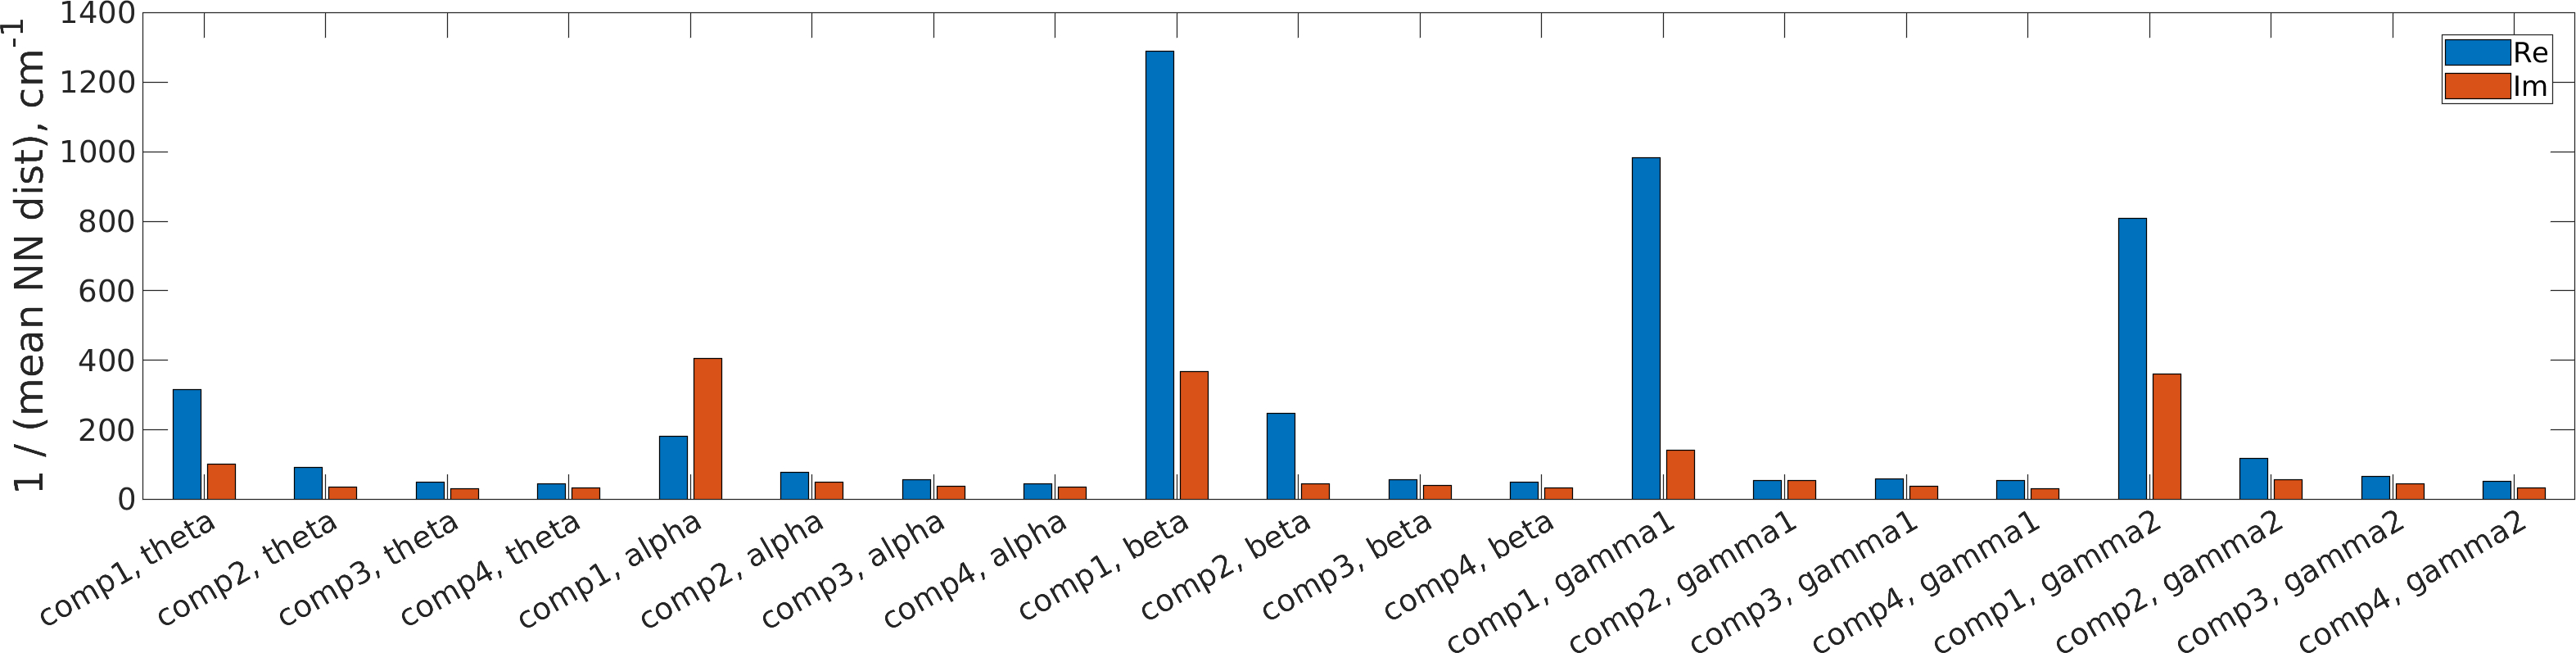
\includegraphics[width=1\textwidth]{../images/psiicos_paper/Figure10_hr.jpg}
 \caption{Полосы частот с наиболее воспроизводимыми сетями, определенными при помощи
 процедуры бутстрэпа.}\label{fig:10}
 Бутстрэп проводился последовательным выбором подмножества эпох, на котором
 вычислялся кросс-спектр, к которому затем применялась PSIICOS-проекция.
 Столбики на графике отображают индекс воспроизводимости, который вычислялся
 как обратное к среднему расстоянию до ближайшего соседа для каждой отдельной
 сети, найденной по мнимой и действительной спроецированной части кросс-спектра для четырех
 наиболее значимых главных компонент. Результаты для действительной части представлены
 синим цветом, а для мнимой~--- желтым.
 \end{figure} %Figure 10

 На графиках~\ref{fig:11},~\ref{fig:12},~\ref{fig:13} изображена пространственная
структура обнаруженных сетей для этих частотных диапазонов. Сети, узлы которых
оказывались ближе 1 сантиметра друг к другу, мы рисовали одним цветом. Перекрывающиеся сети
мы рисовали с увеличенным размером маркера и увеличенной толщиной линии. Прозрачность
линии мы меняли в зависимости от плотности сетей в кластере с учетом перекрытий.
Также для каждой воспроизводимой компоненты мы рисовали профиль ее временной активации
как правый собственный вектор сингулярного разложения соответствующей части временного
ряда кросс-спектра.

\begin{figure}
\centering
\text{Тета- (3--6 Гц) и альфа- (8--12 Гц) диапазоны}

 \begin{subfigure}[b]{0.4\textwidth}
 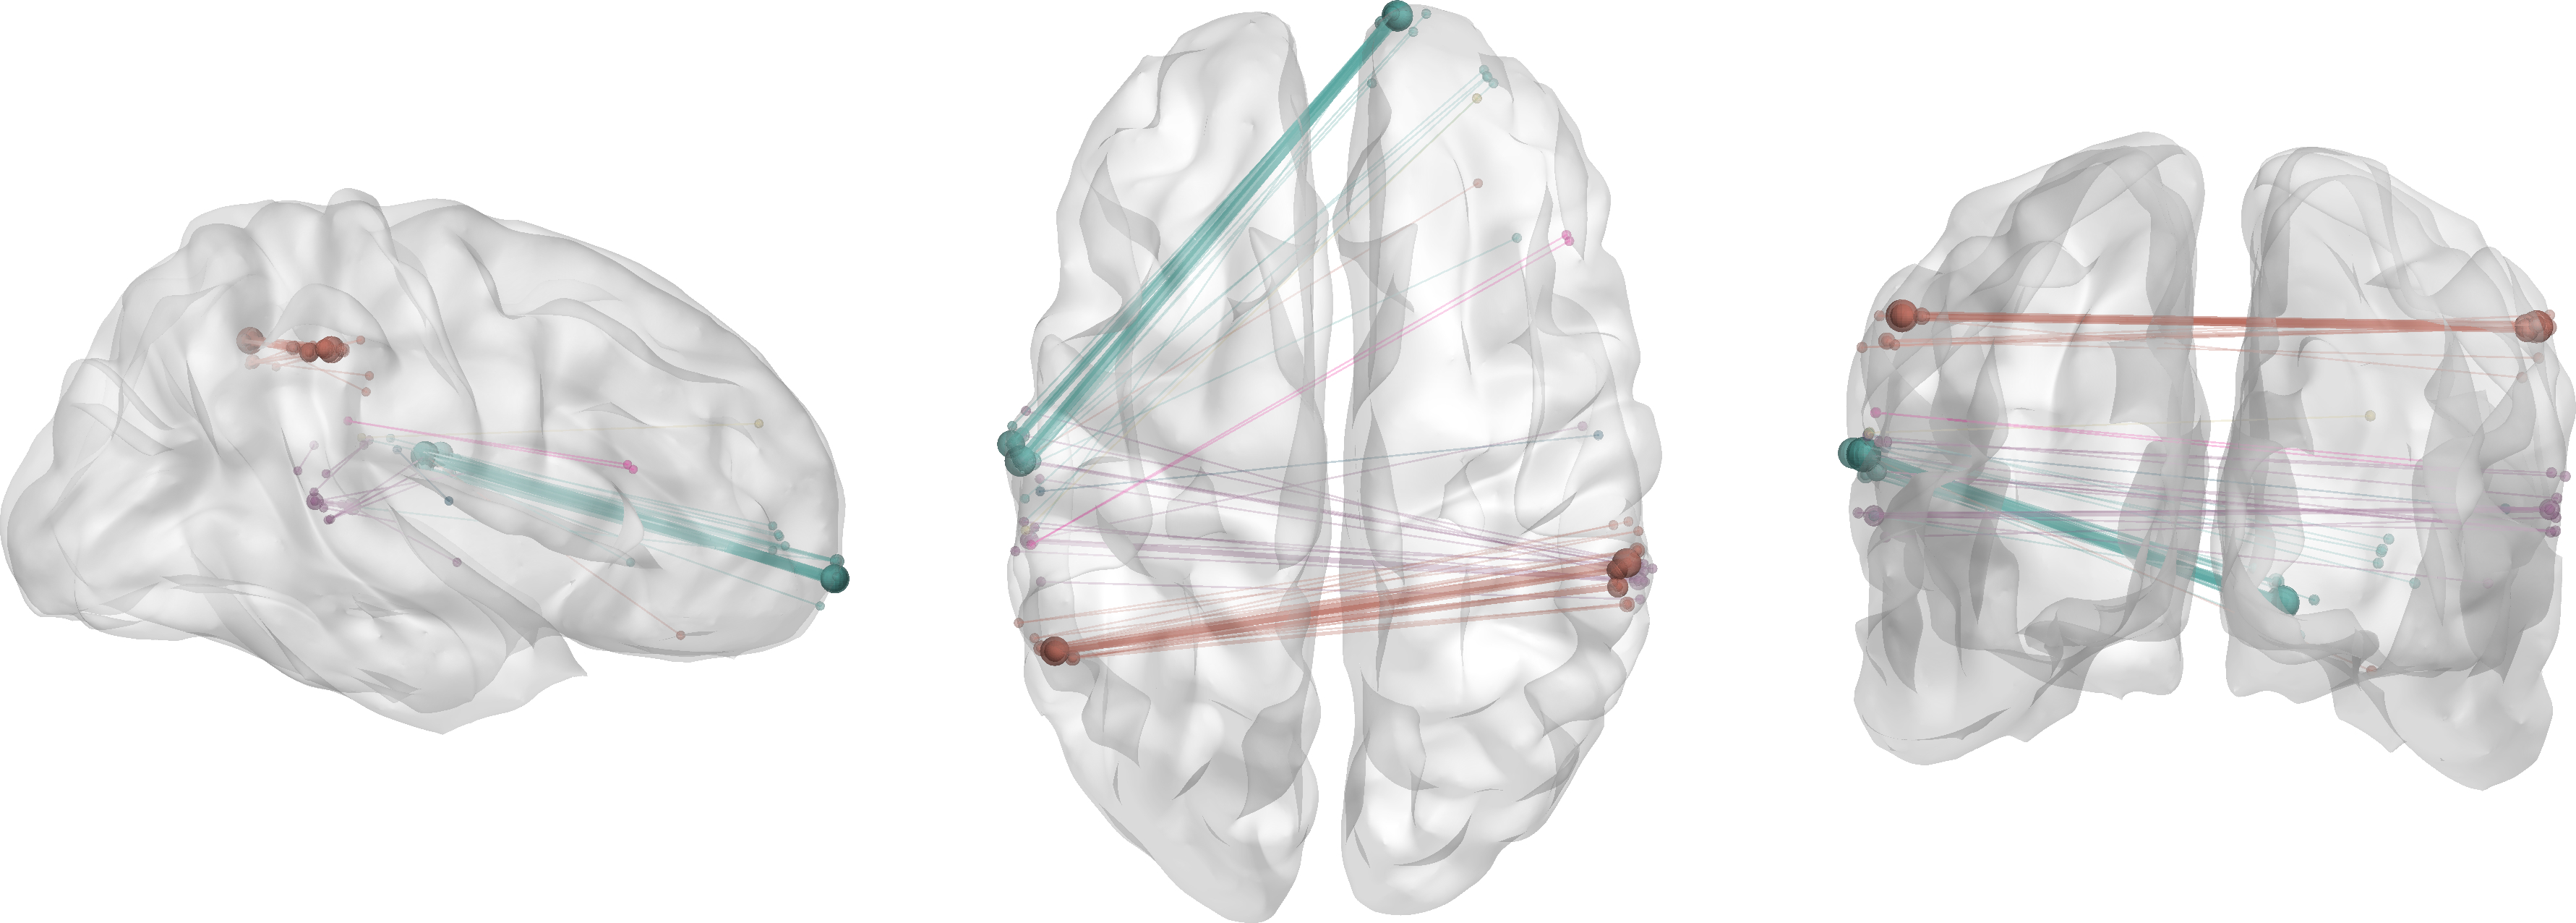
\includegraphics[width=\textwidth]{../images/psiicos_paper/Figure11_a1.jpg}
 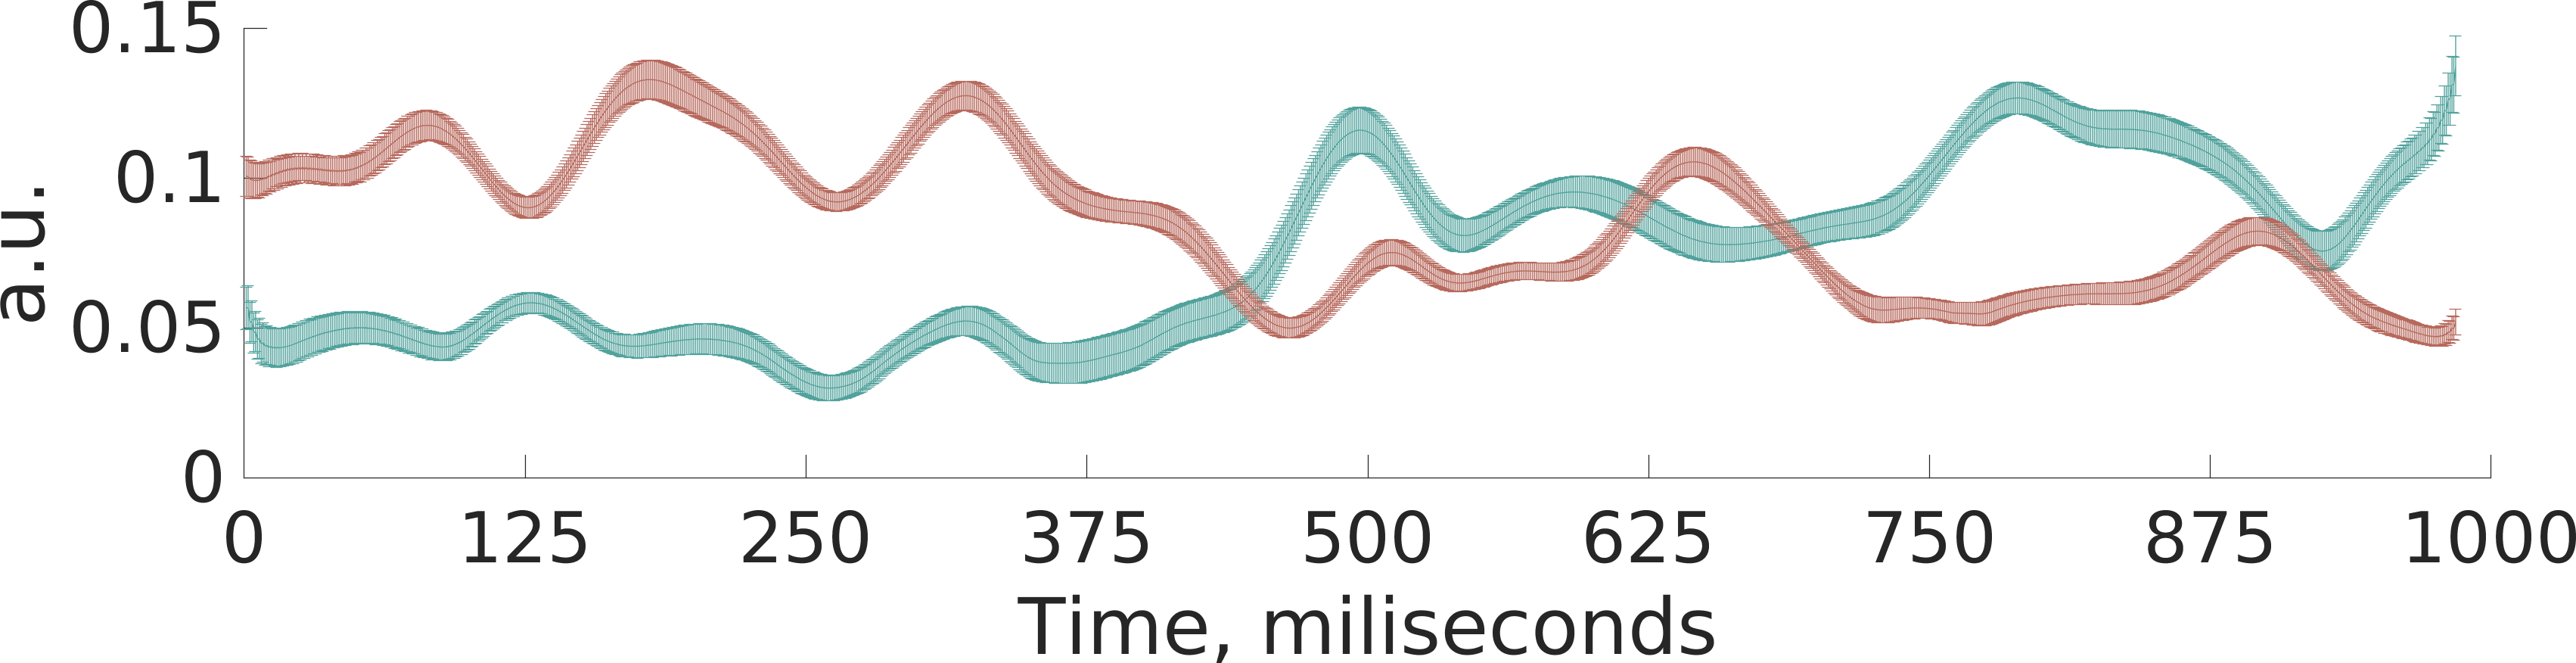
\includegraphics[width=\textwidth]{../images/psiicos_paper/Figure11_a2.jpg}
 \caption{Тета-диапазон, Re, сеть 1}\label{fig:11a}
 \end{subfigure}
 \hspace{1cm}
 \begin{subfigure}[b]{0.4\textwidth}
 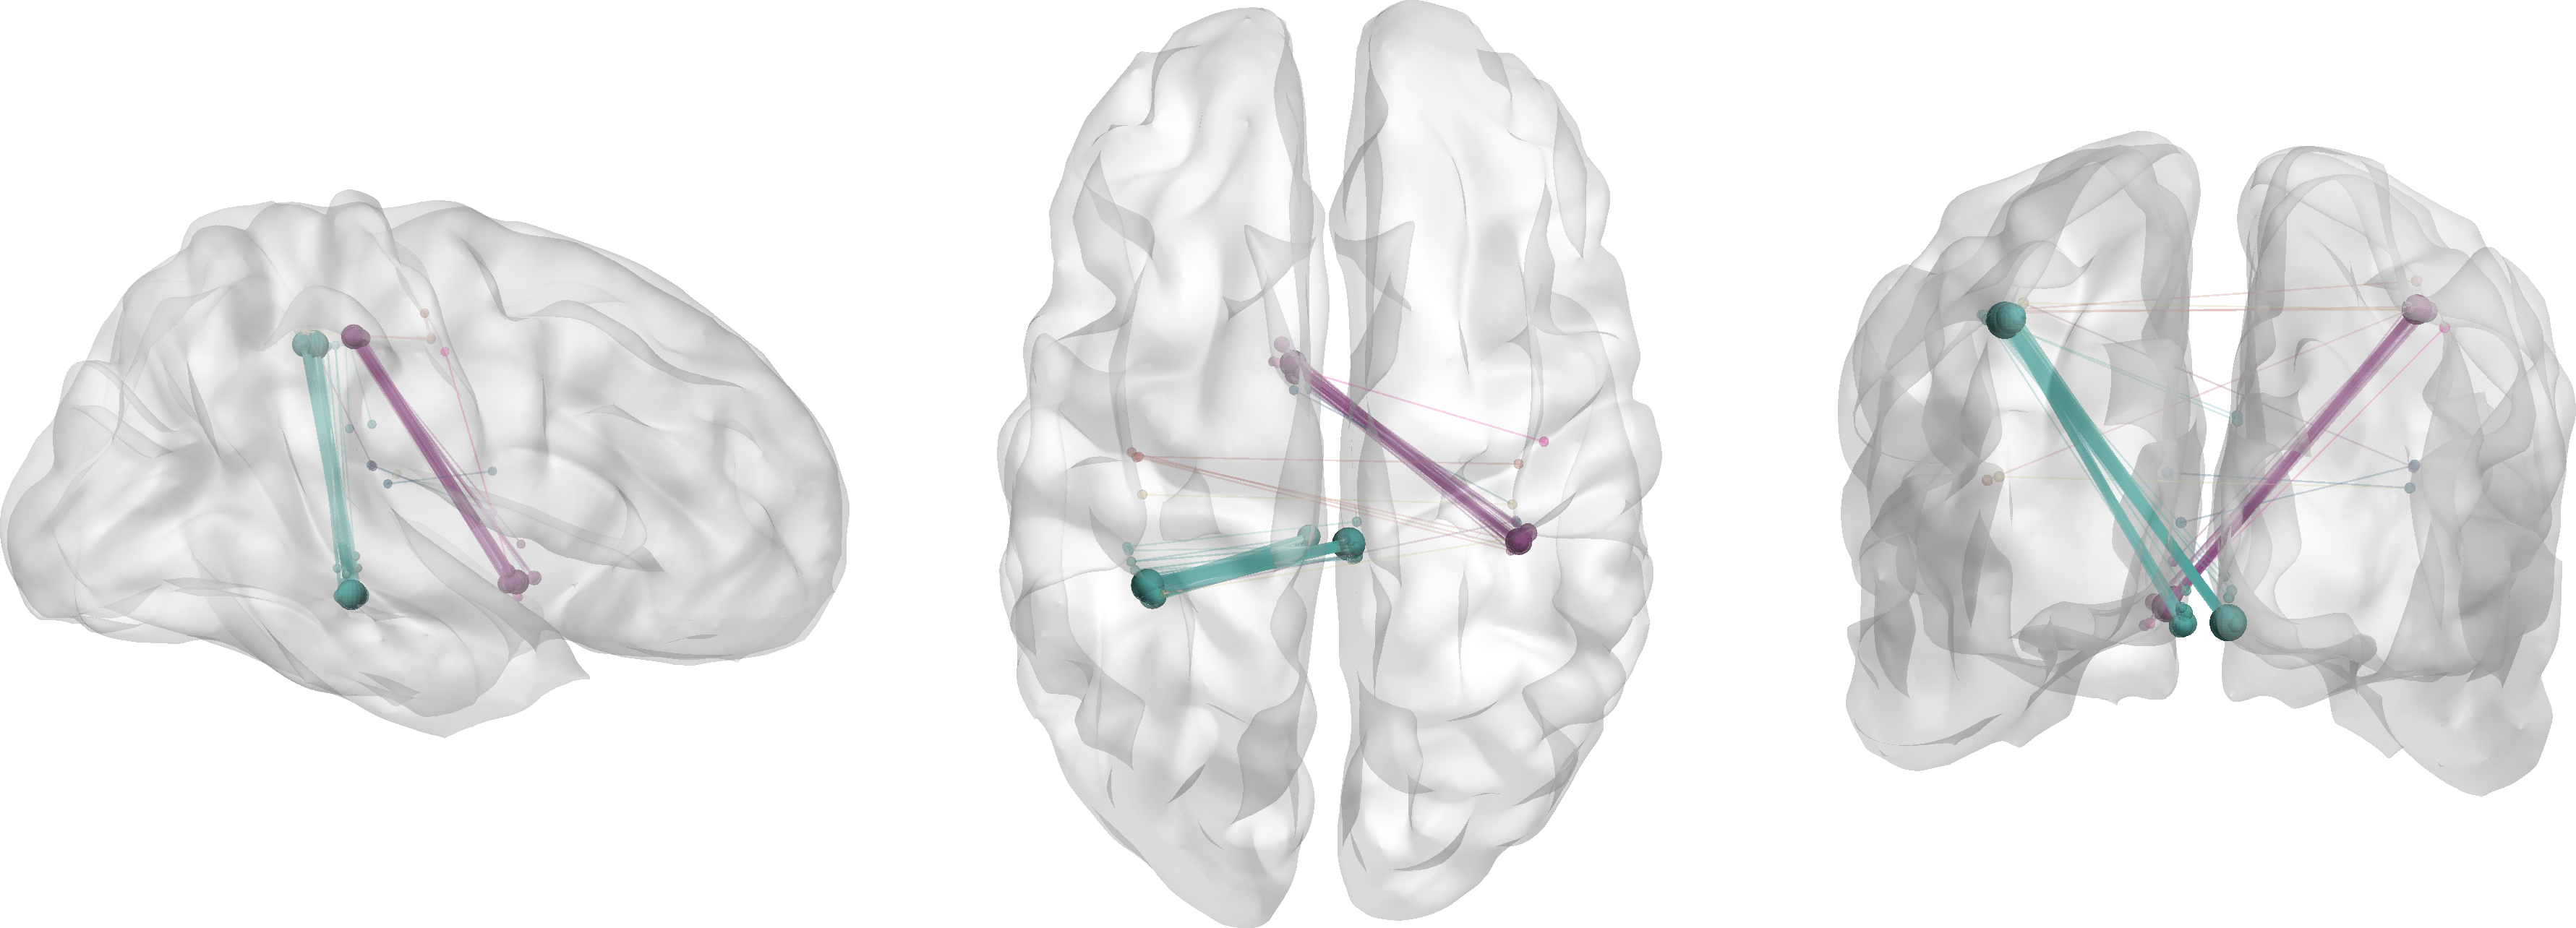
\includegraphics[width=\textwidth]{../images/psiicos_paper/Figure11_b1.jpg}
 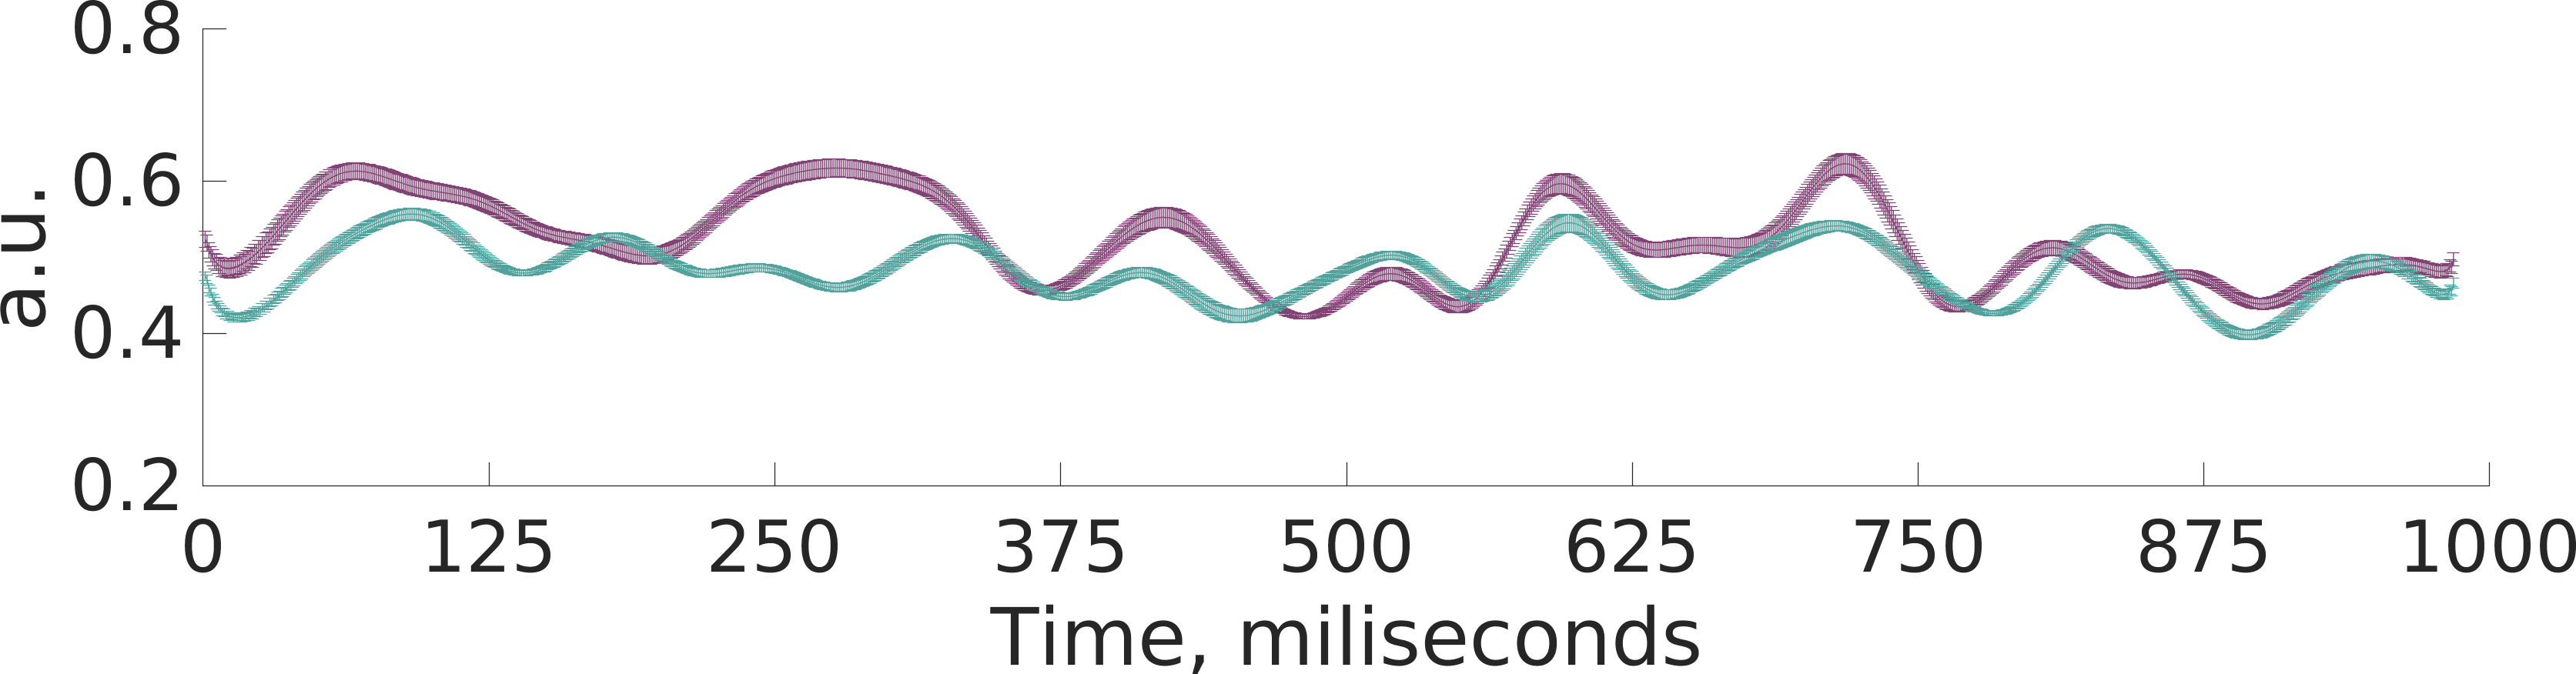
\includegraphics[width=\textwidth]{../images/psiicos_paper/Figure11_b2.jpg}
 \caption{Альфа-диапазон, Im, сеть 1}\label{fig:11b}
 \end{subfigure}
 \caption{Пространственная структура и временная динамика наиболее воспроизводимых сетей в диапазонах частот тета (3--6 Гц) и альфа (8--12 Гц)}\label{fig:11}
\end{figure} % figure 11

Анализ действительной части кросс-спектра показывает наличие следующих сетей с преимущественно
малыми фазовыми задержками. В тета-диапазоне (рис.~\ref{fig:11}) мы видим сети,
соединяющие правую орбито-фронтальную кору, вовлеченную в сенсорную интеграцию, с левым
билатеральным височно-теменным узлом, про который известно, что он активен при воображении
движения~(\cite{Hanakawa2008}). Также мы видим кросс-латеральную сеть, соединяющую два
теменных отдела.

В бета-диапазоне мы видим механистически правдоподобную кросс-латеральную связь
между вентральным зрительным путем и зоной репрезентации руки в моторной
области правого полушария. Дополнительно мы наблюдаем взаимодействие между
зонами представительства руки сенсомоторной области правого полушария и
соматосенсорной области левого, рис.~\ref{fig:12}, что частично
согласуется с наблюдениями, описанными в статье~\cite{Lamm2007} и соотносится
с профилями функциональной коннективности, описанными в  фМРТ-исследовании
воображаемых вращений~\cite{Striem-Amit2017}. Наконец, мы обнаружили взаимодействие
зоны представительства руки в моторной области правого полушария с височным полюсом
левого полушария в гамма-диапазоне, рис.~\ref{fig:13a}, а также с
орбито-фронтальной зоной левого полушария в верхнем гамма-диапазоне, рис.~\ref{fig:13b}.
Правдоподобность этих наблюдений подкреплена предполагаемой
ролью височного полюса левого полушария, в которую входит ``\ldots визуальное различение
двумерных изображений и мнемоническая функция соотнесения и научения'' (\cite{Dupont2002}).

\begin{figure}
\centering
\text{Бета-диапазон (16--24 Гц)}

 \begin{subfigure}[b]{0.4\textwidth}
 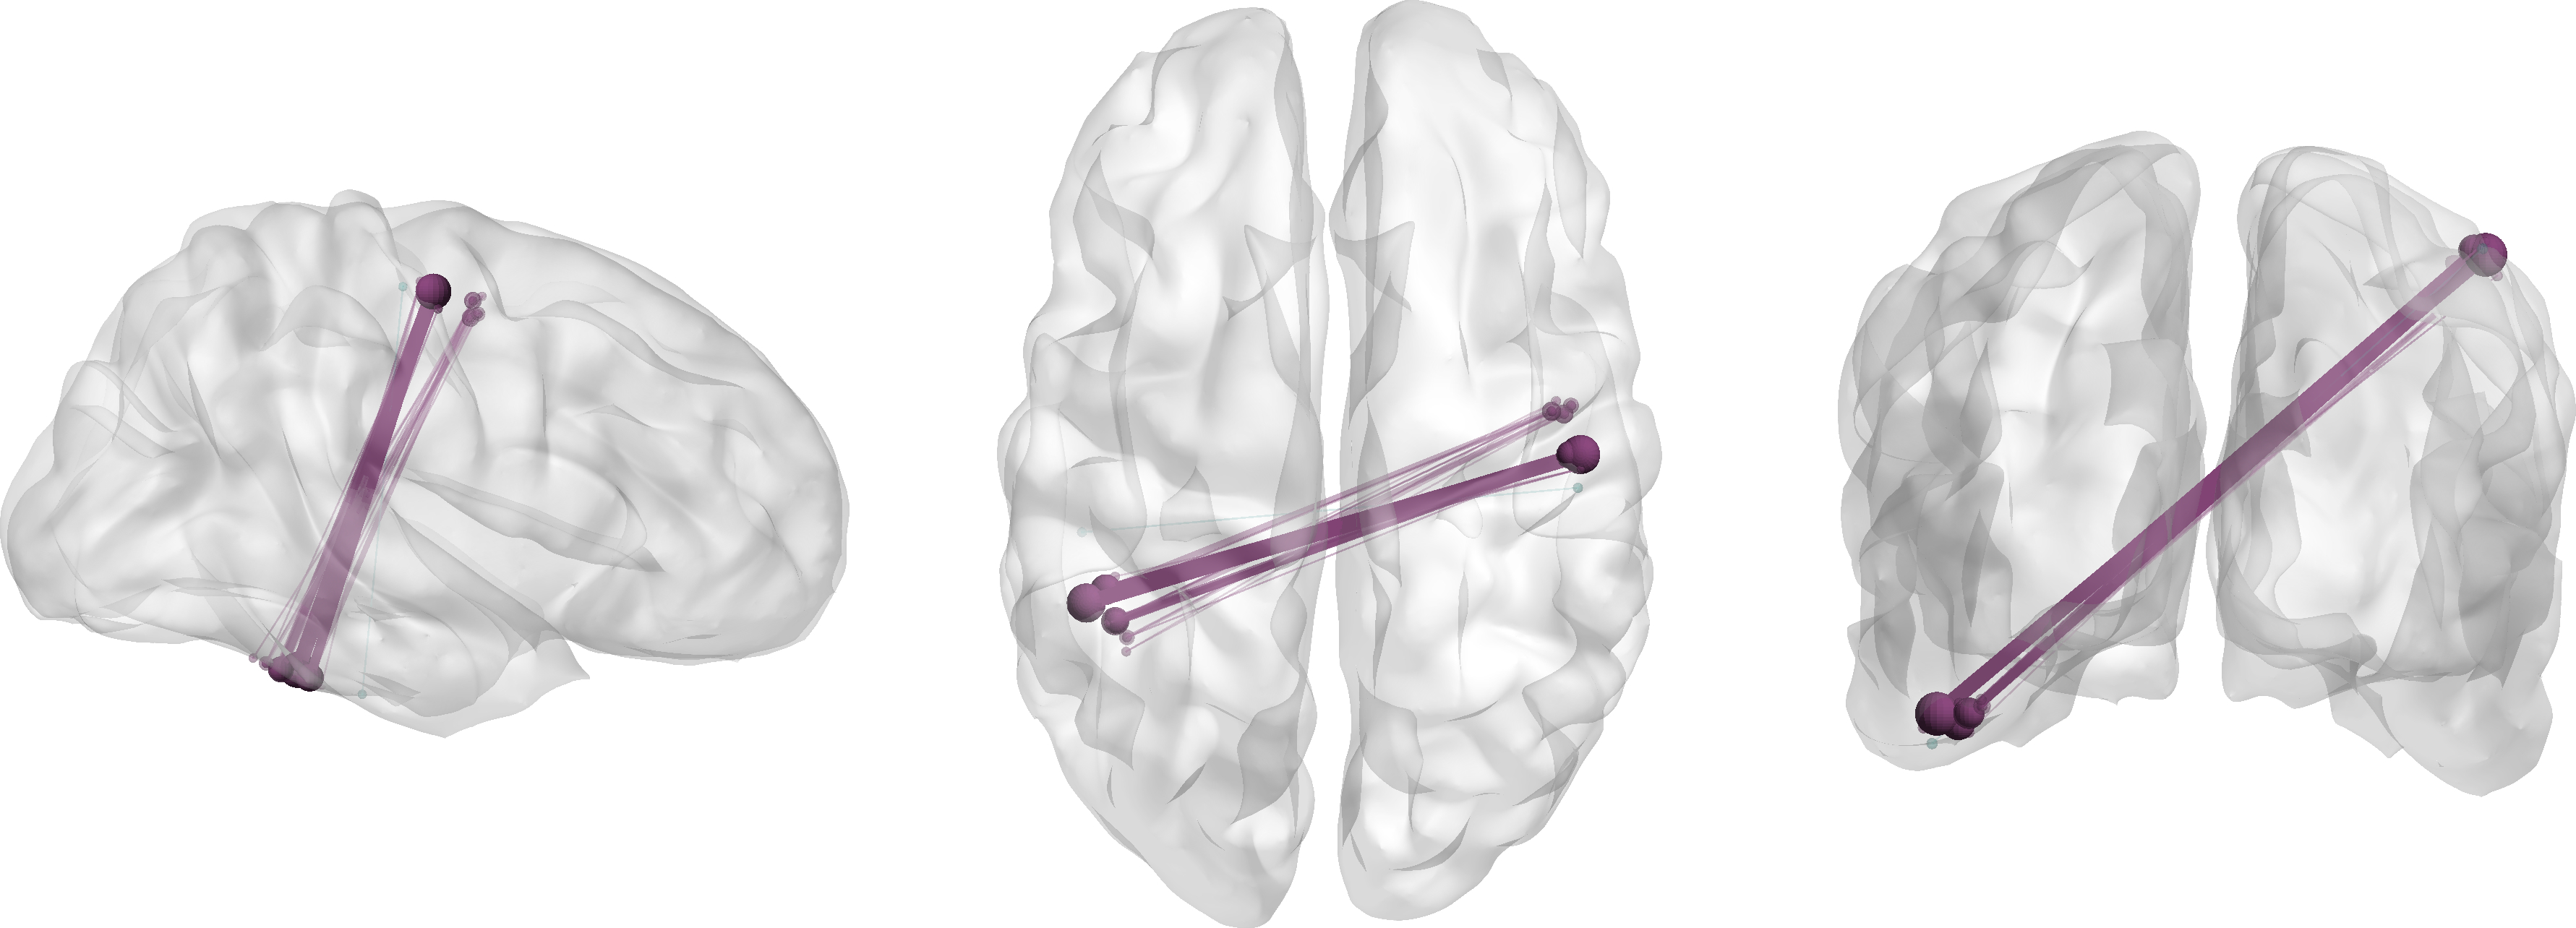
\includegraphics[width=\textwidth]{../images/psiicos_paper/Figure12_a1.jpg}
 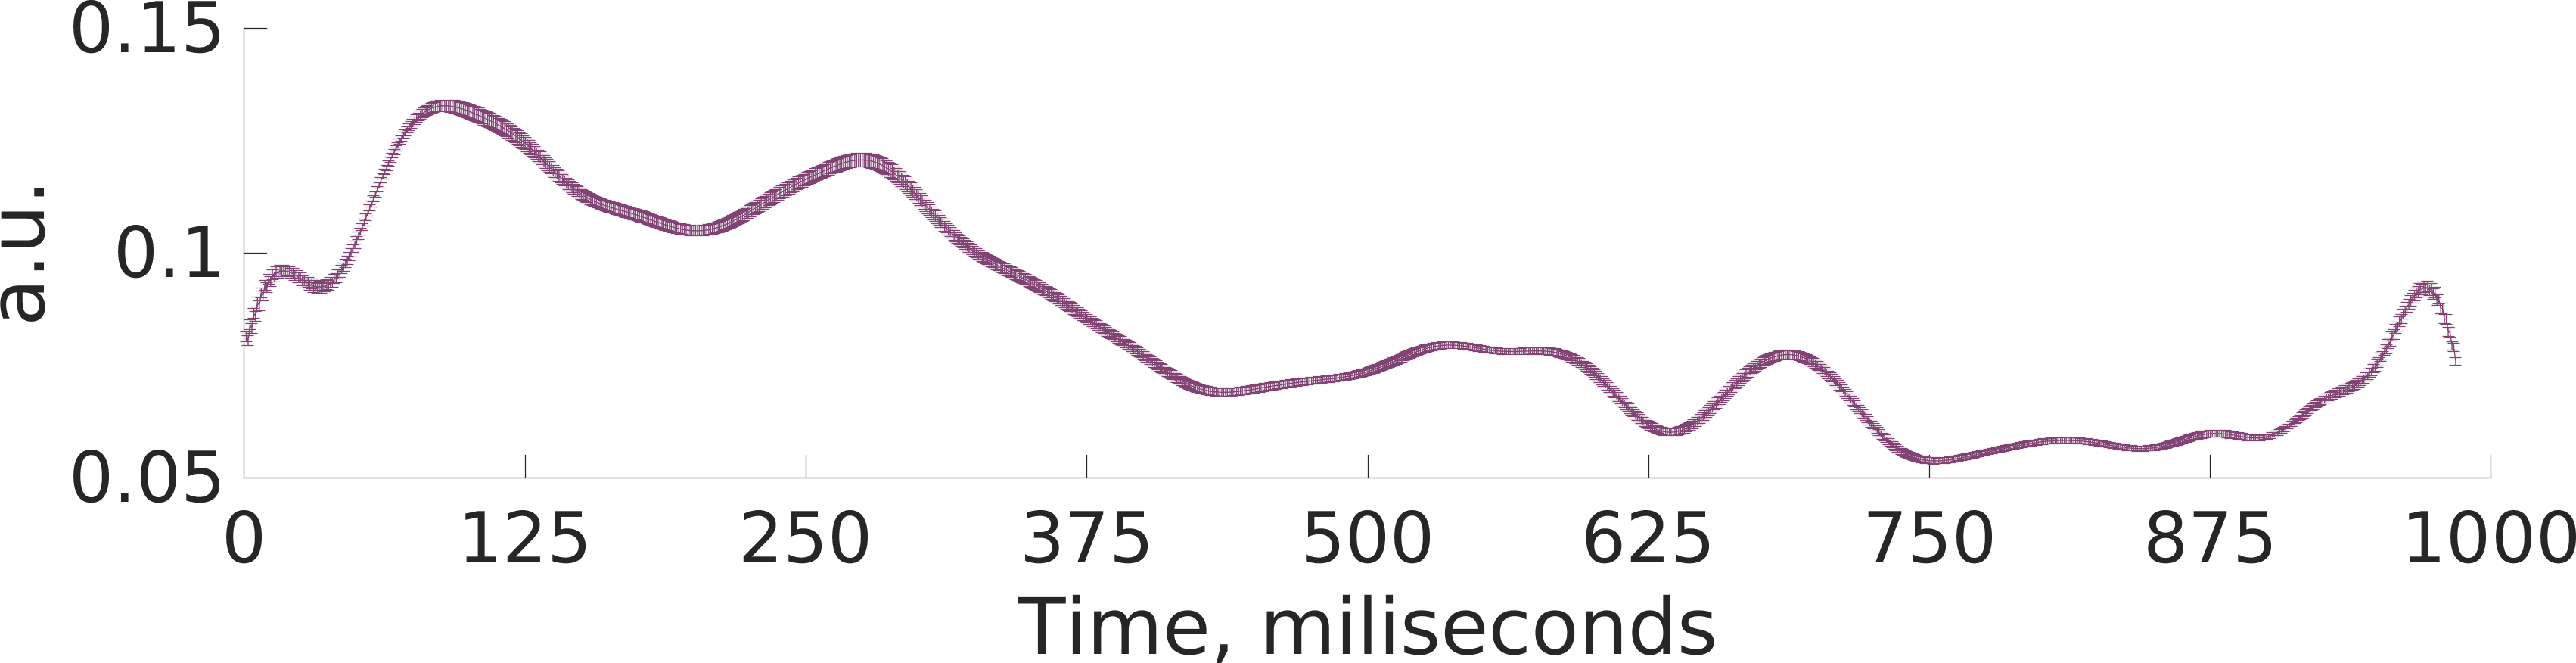
\includegraphics[width=\textwidth]{../images/psiicos_paper/Figure12_a2.jpg}
 \caption{Re, сеть 1}\label{fig:12a}
 \end{subfigure}
 \hspace{1cm}
 \begin{subfigure}[b]{0.4\textwidth}
 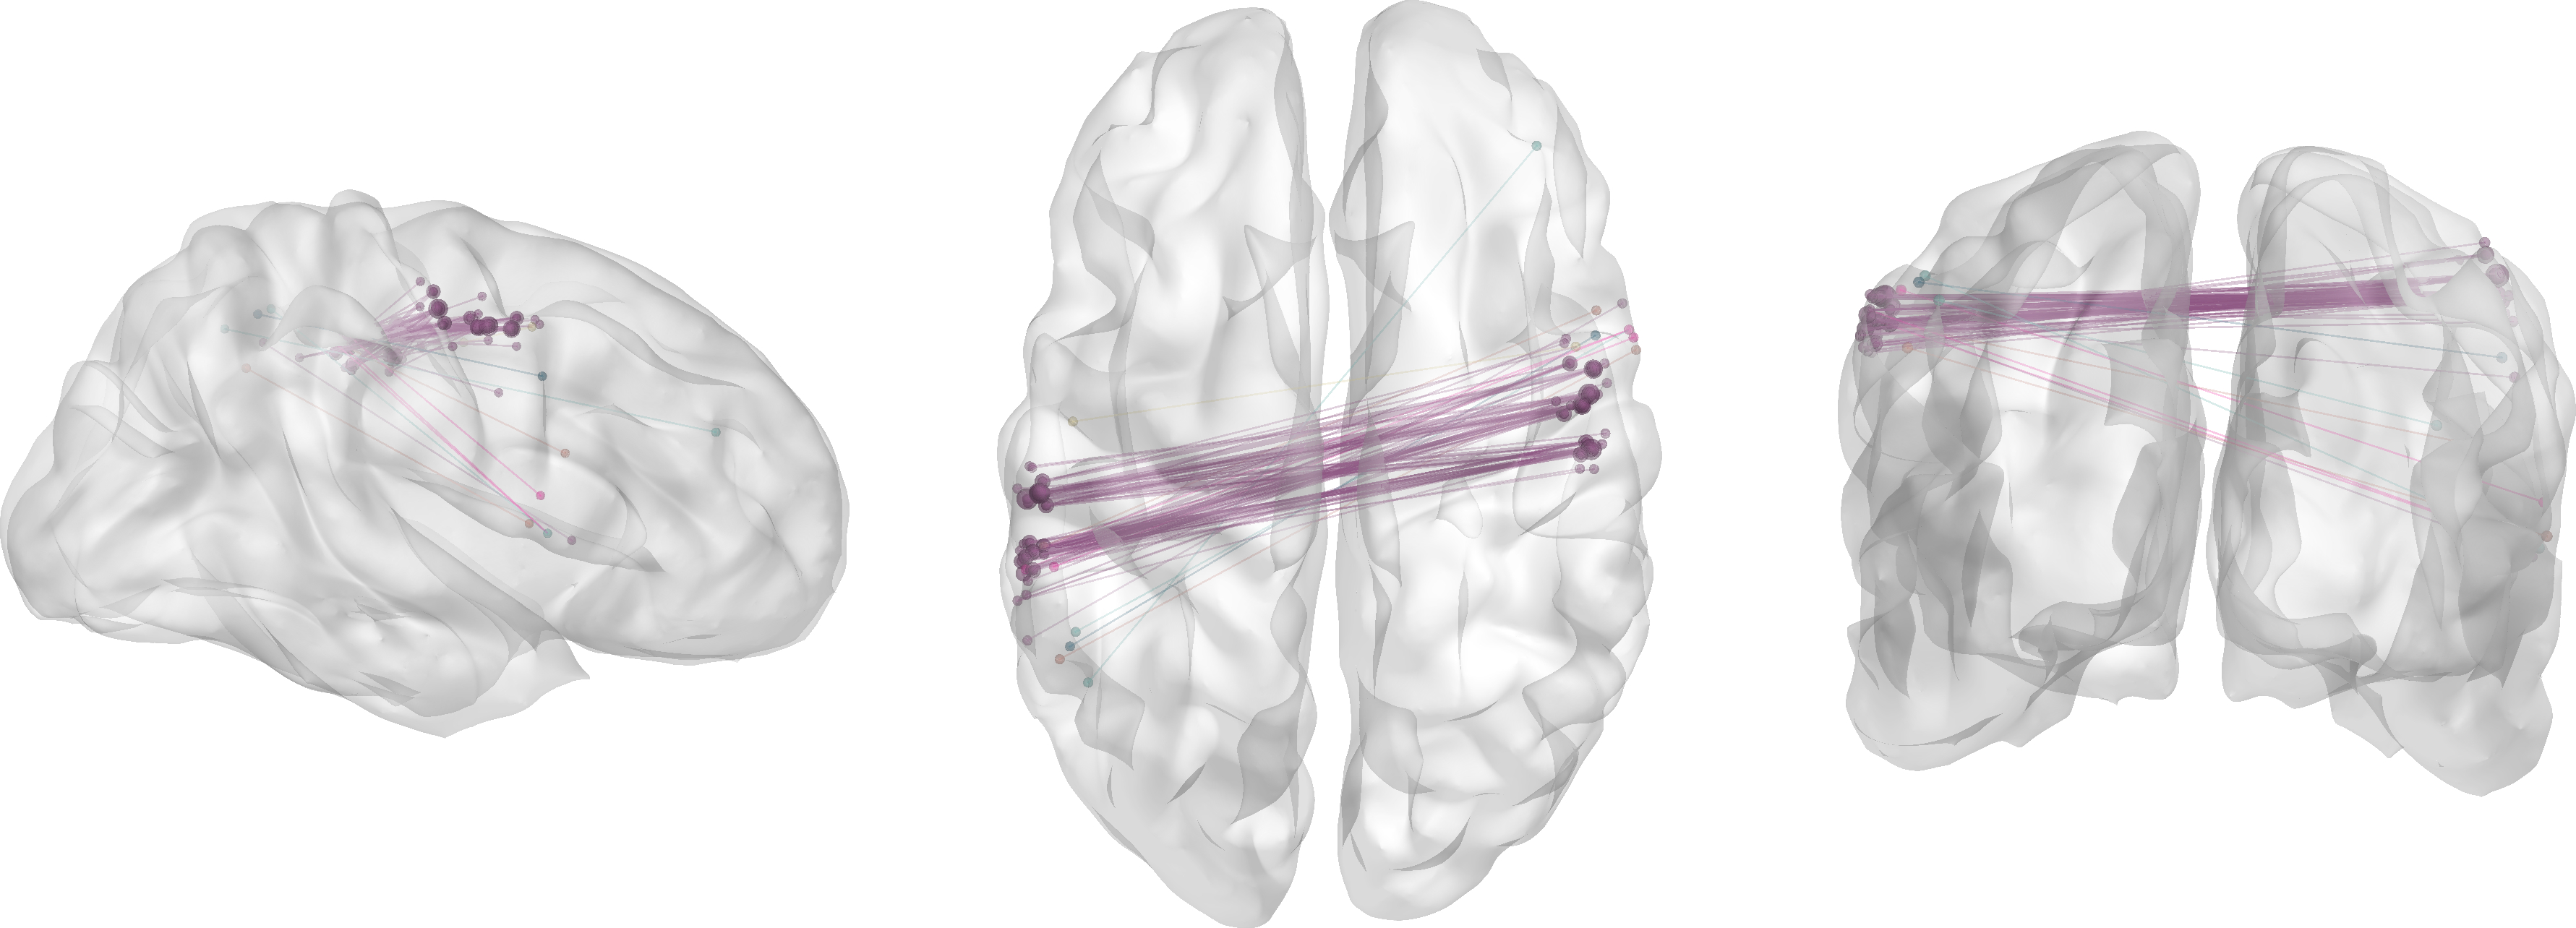
\includegraphics[width=\textwidth]{../images/psiicos_paper/Figure12_b1.jpg}
 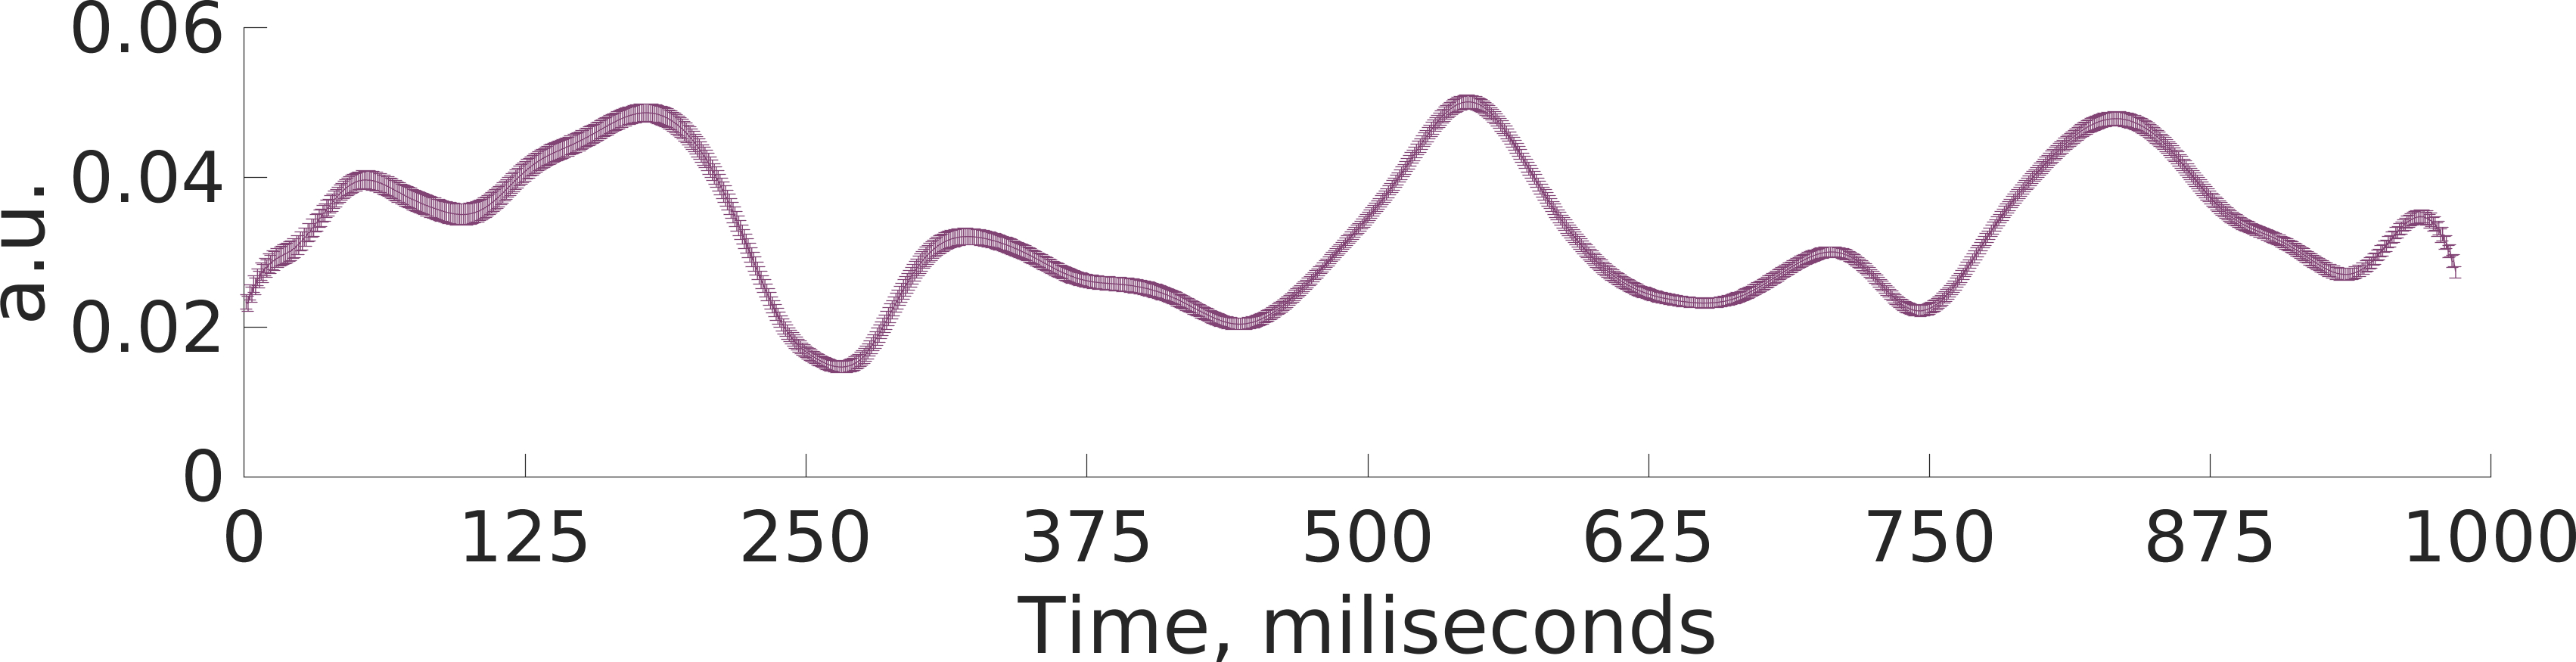
\includegraphics[width=\textwidth]{../images/psiicos_paper/Figure12_b2.jpg}
 \caption{Re, сеть 2}\label{fig:12b}
 \end{subfigure}
 \begin{subfigure}[b]{0.4\textwidth}
 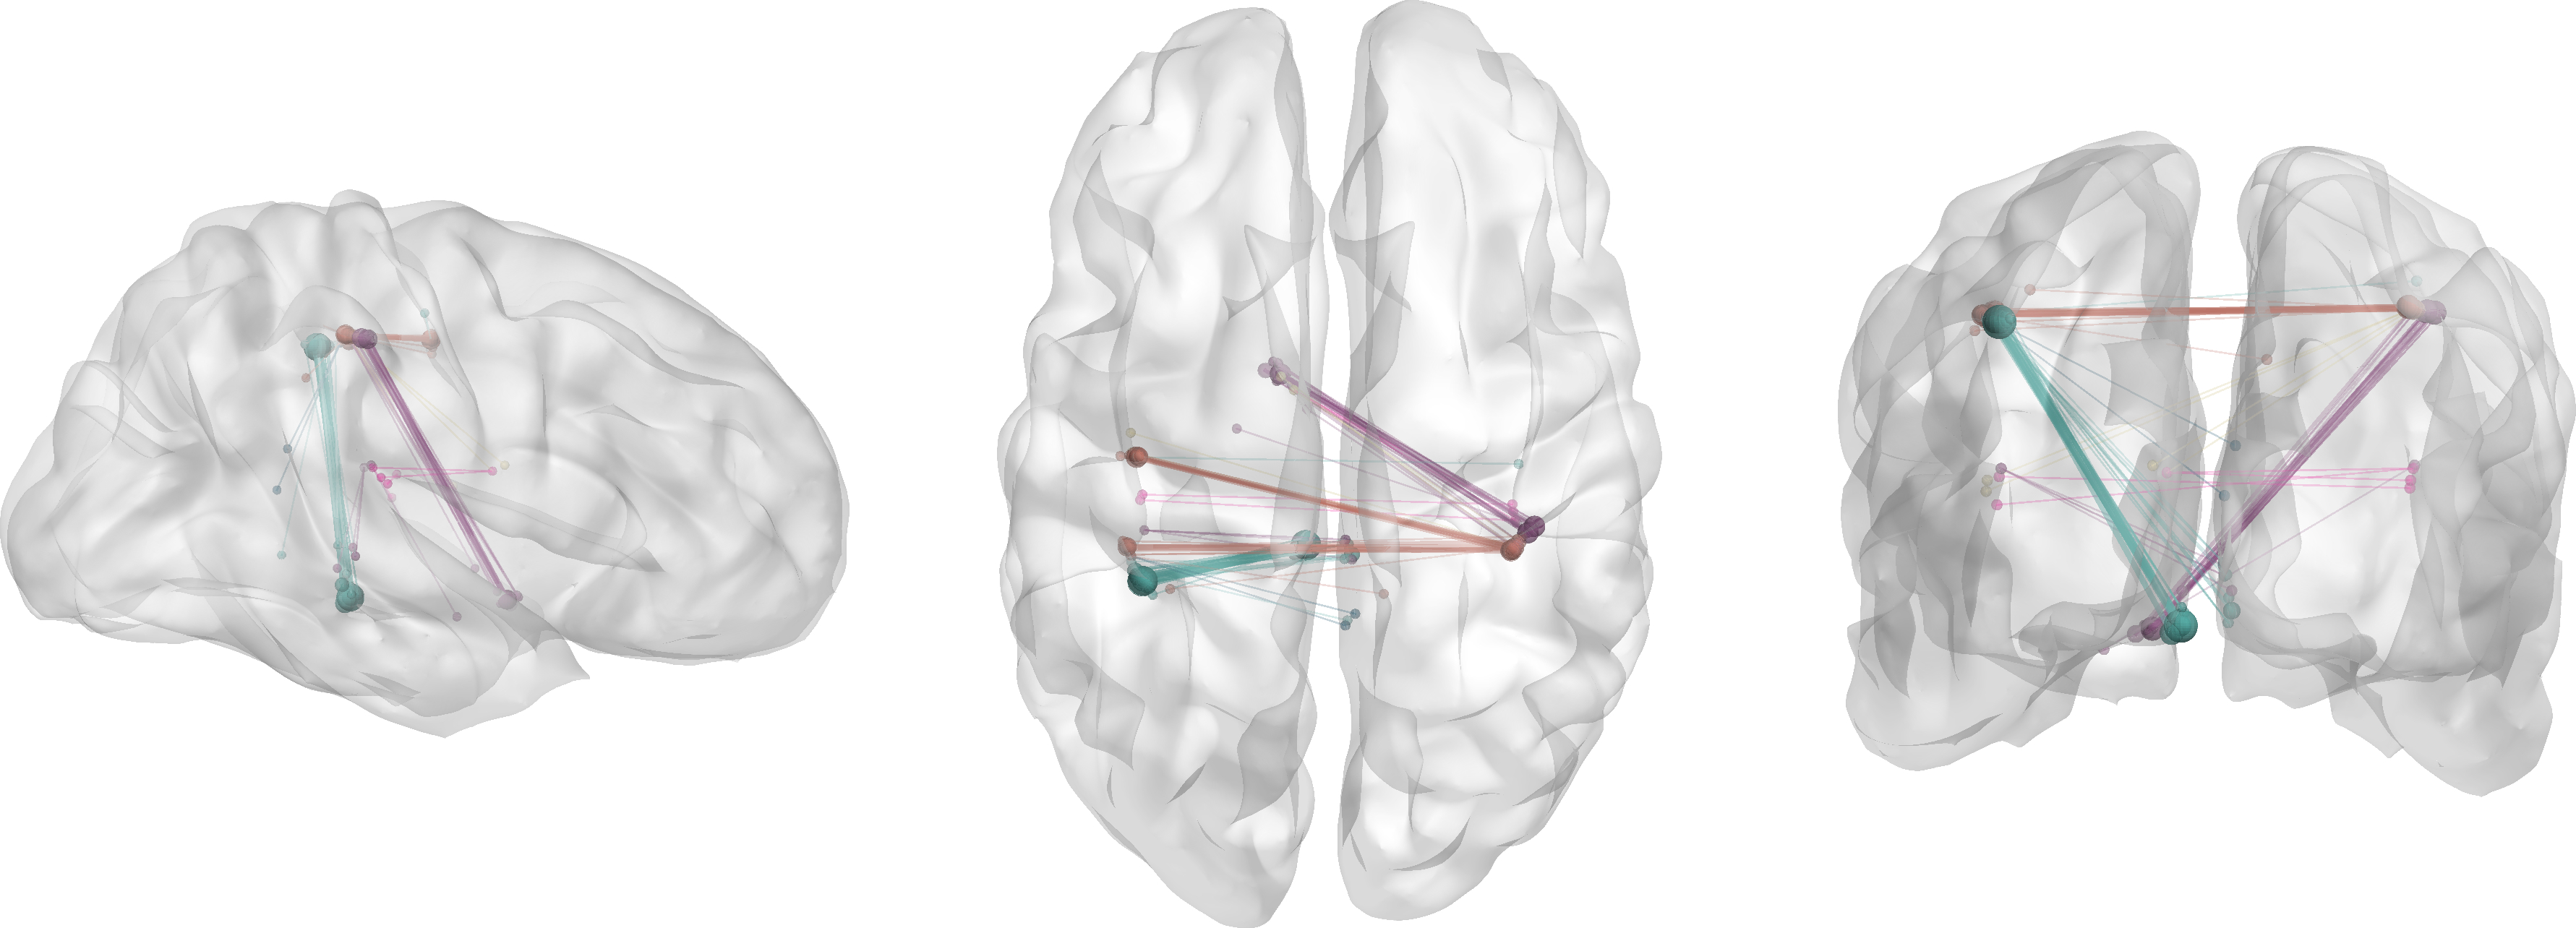
\includegraphics[width=\textwidth]{../images/psiicos_paper/Figure12_c1.jpg}
 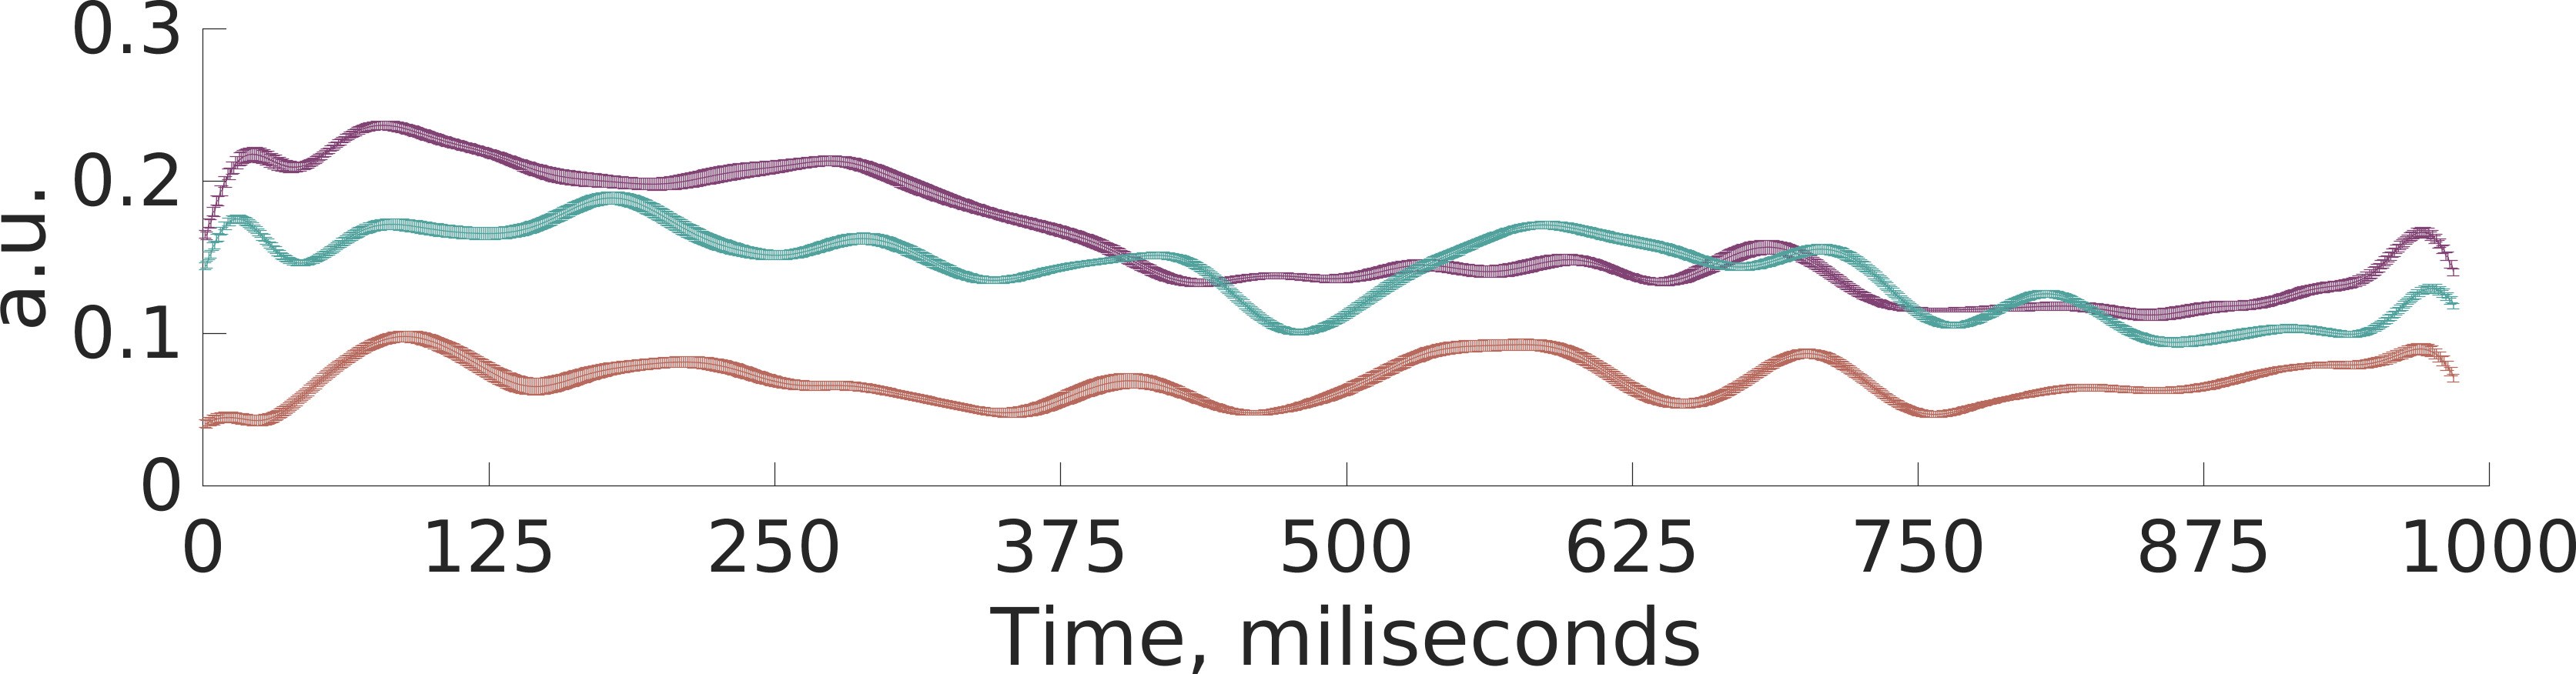
\includegraphics[width=\textwidth]{../images/psiicos_paper/Figure12_c2.jpg}

 \caption{Im, сеть 1}\label{fig:12c}
 \end{subfigure}
 \caption{Пространственная структура и временная динамика наиболее воспроизводимых сетей в бета-диапазоне (16--24 Гц)}\label{fig:12}
\end{figure} %figure 12

\begin{figure}
\centering
\text{Нижний (30--60 Гц) и верхний (65--85 Hz) гамма-диапазоны}

 \begin{subfigure}[b]{0.4\textwidth}
 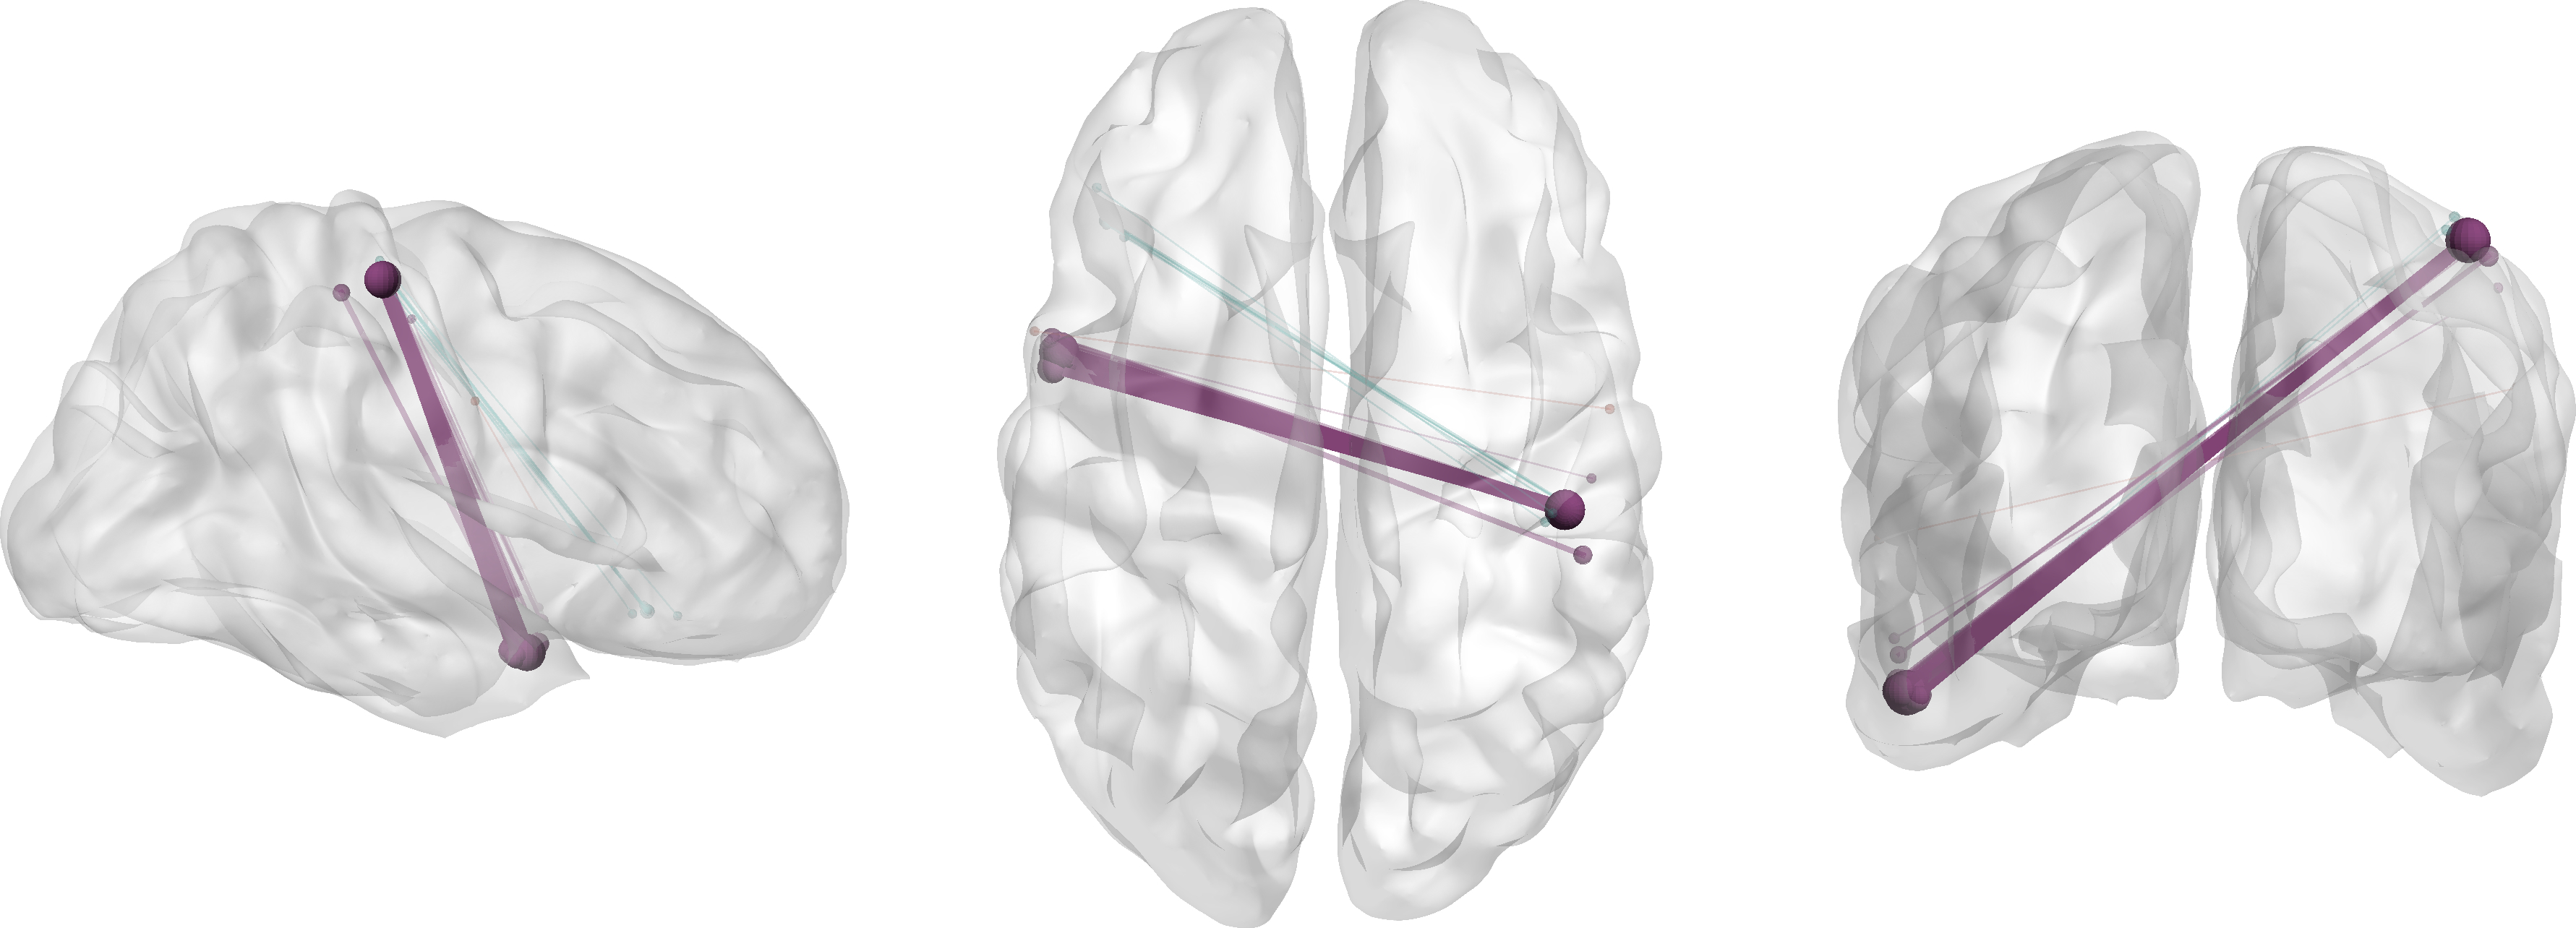
\includegraphics[width=\textwidth]{../images/psiicos_paper/Figure13_a1.jpg}
 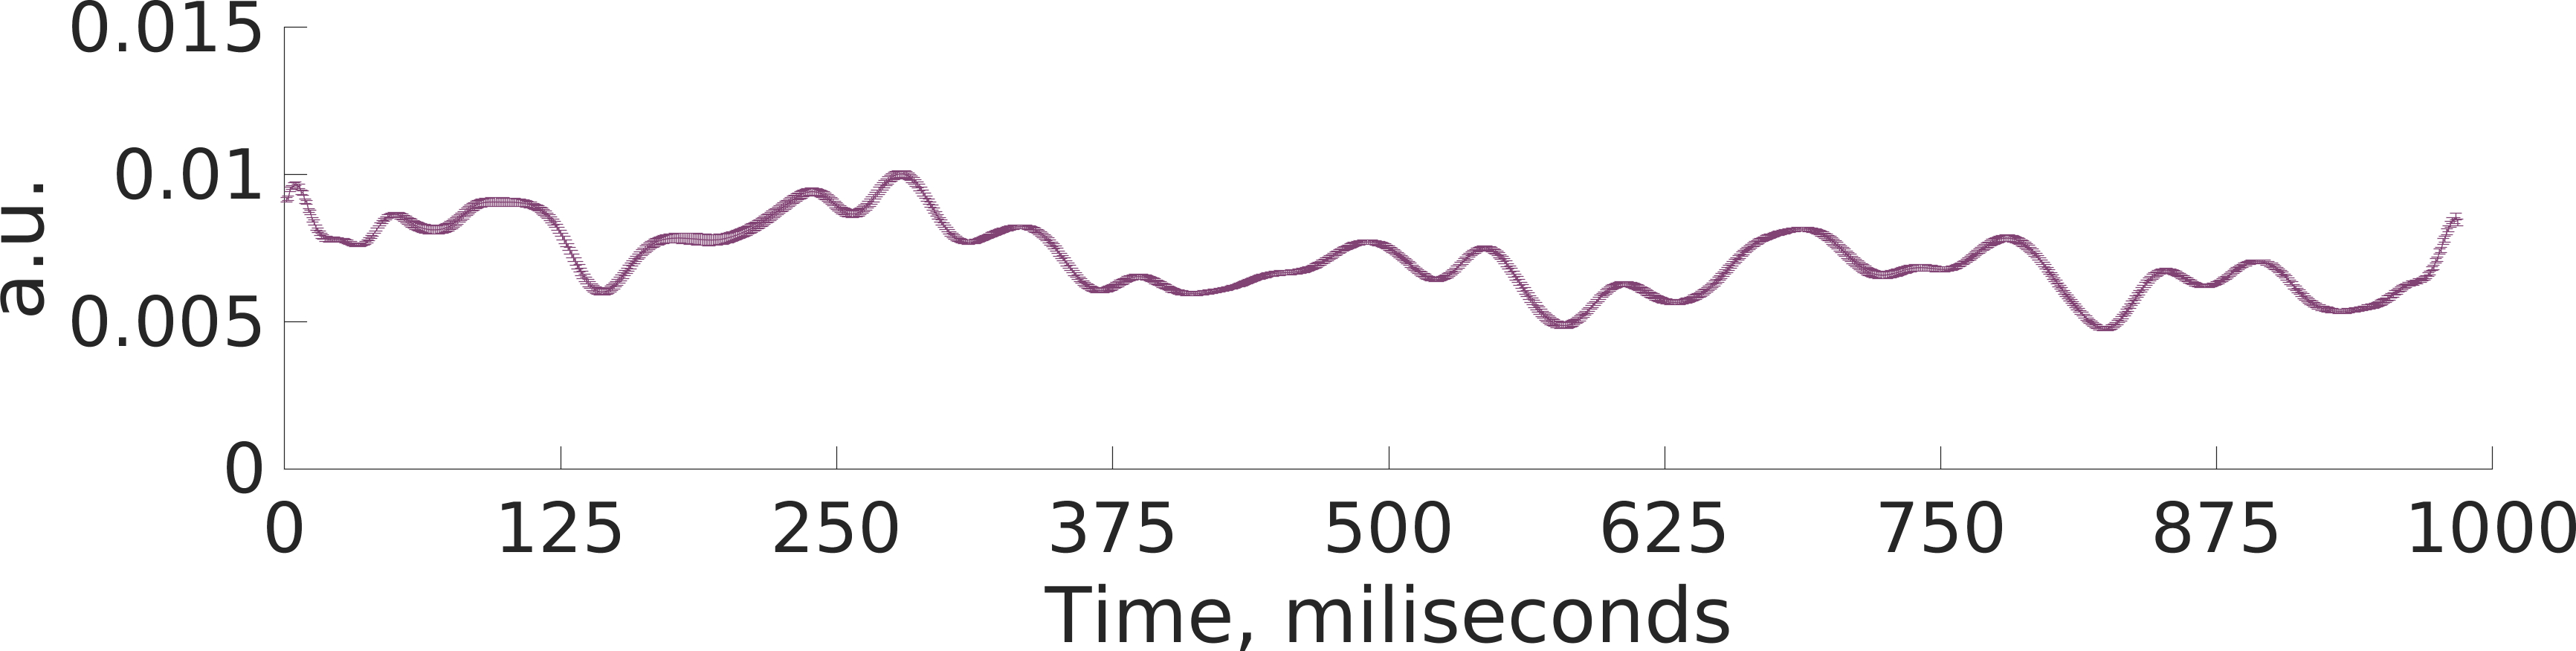
\includegraphics[width=\textwidth]{../images/psiicos_paper/Figure13_a2.jpg}
 \caption{Ниж. гамма-диапазон, Re, сеть 1}\label{fig:13a}
 \end{subfigure}
 \hspace{1cm}
 \begin{subfigure}[b]{0.4\textwidth}
 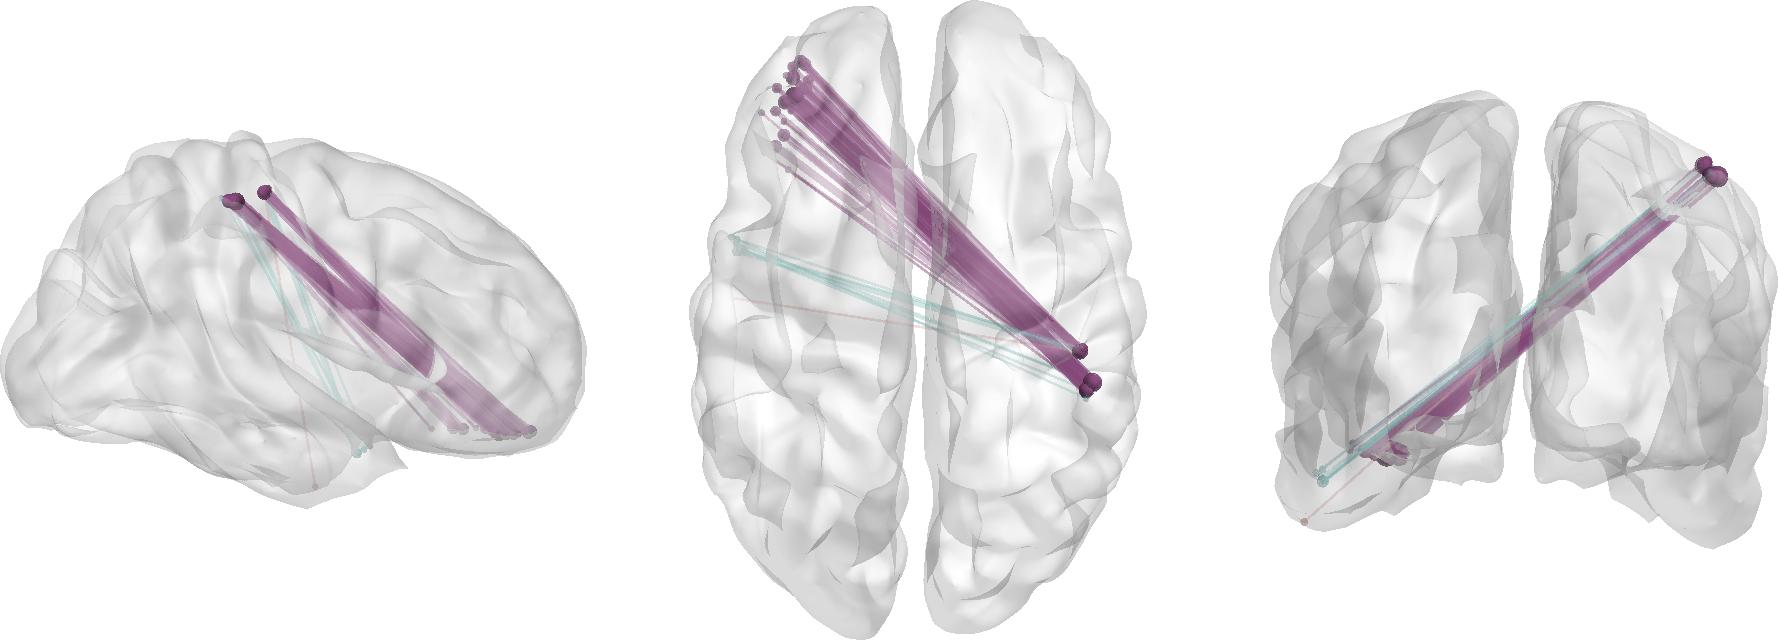
\includegraphics[width=\textwidth]{../images/psiicos_paper/Figure13_b1.jpg}
 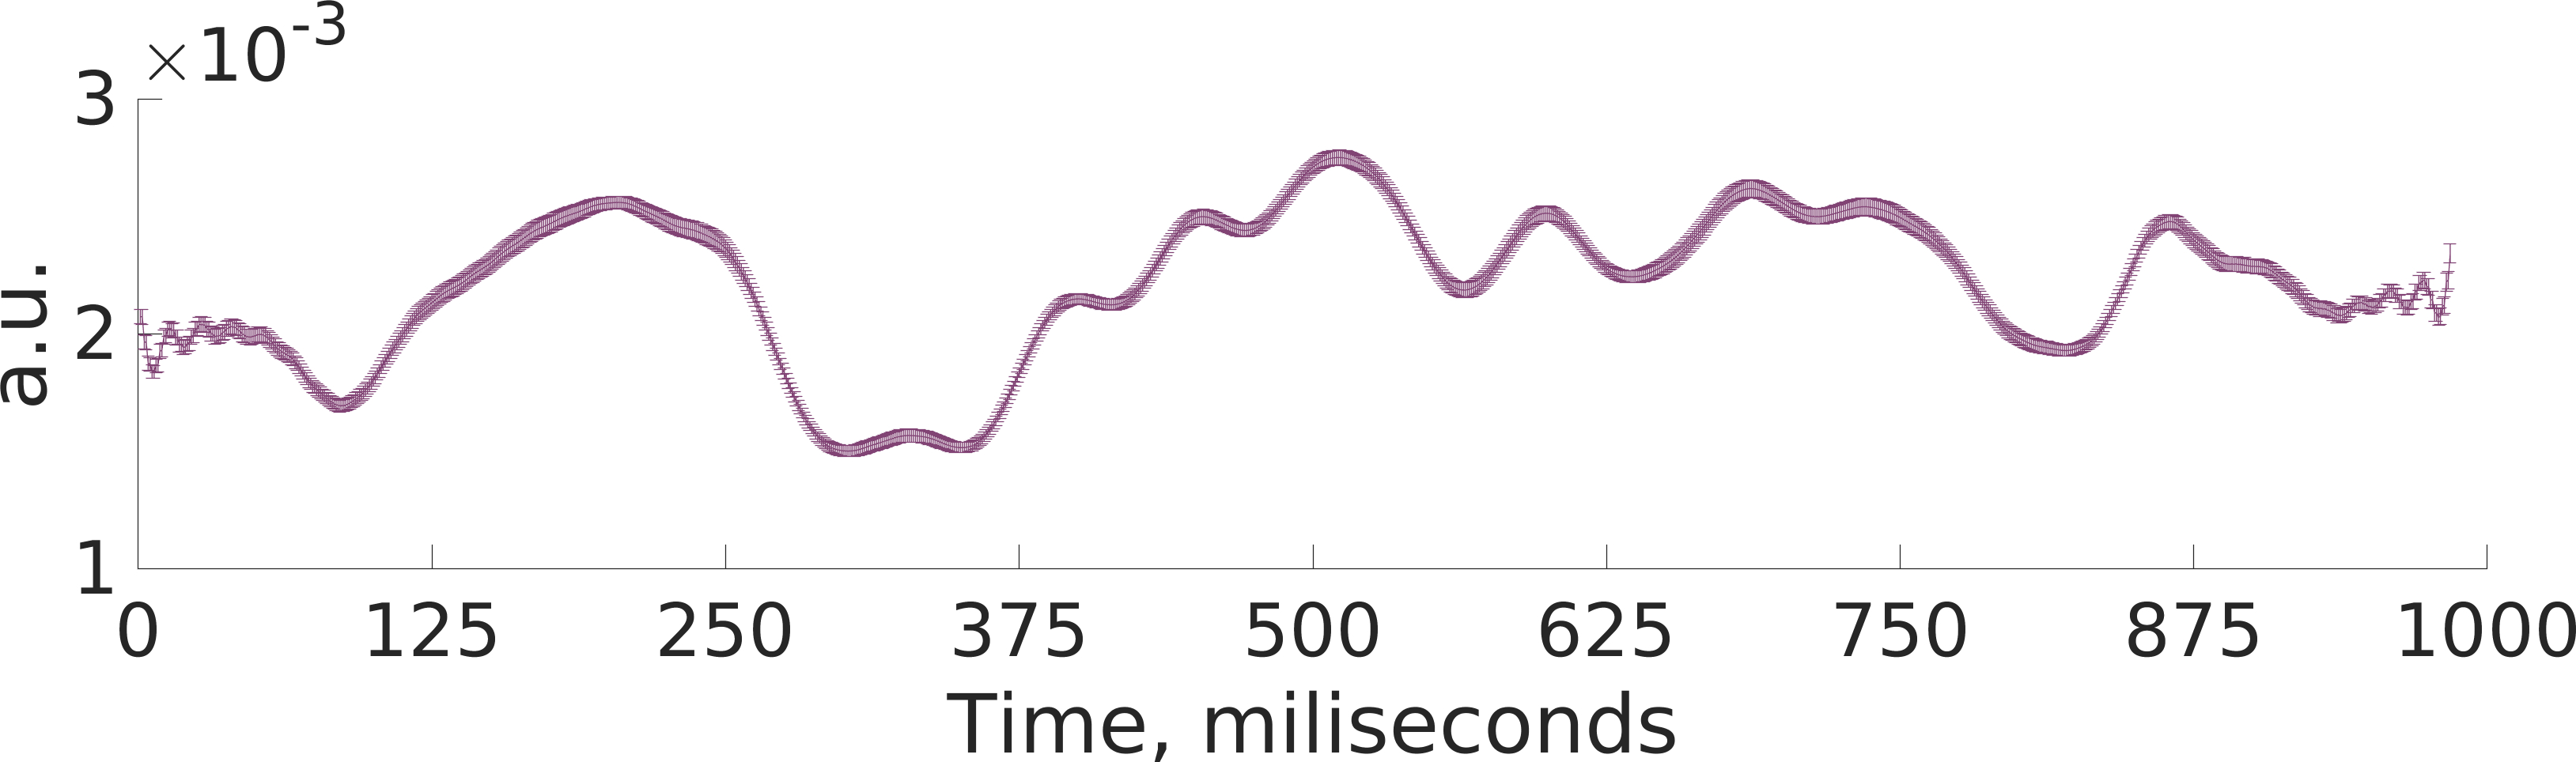
\includegraphics[width=\textwidth]{../images/psiicos_paper/Figure13_b2.jpg}
 \caption{Верх. гамма-диапазон, Re, сеть 1}\label{fig:13b}
 \end{subfigure}

 \begin{subfigure}[b]{0.4\textwidth}
 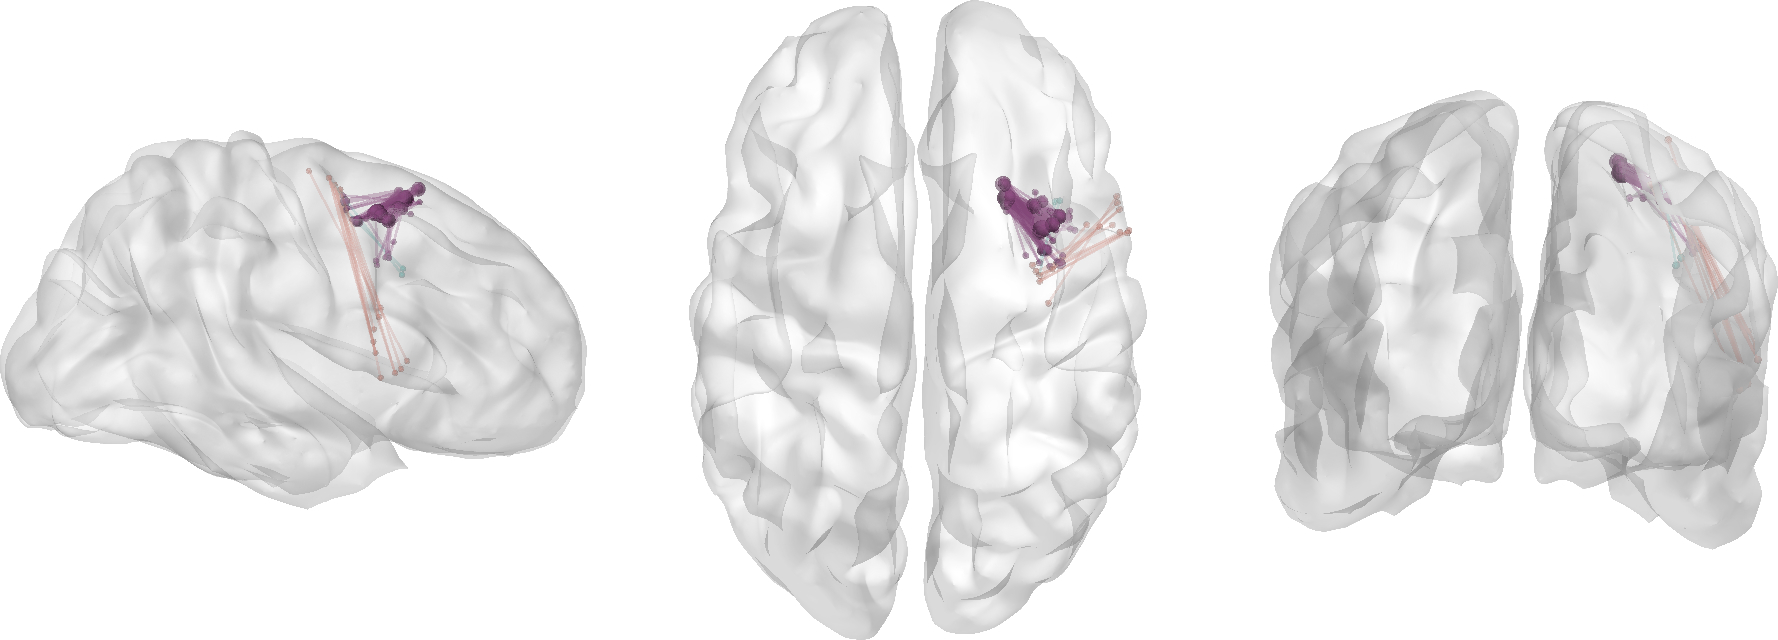
\includegraphics[width=\textwidth]{../images/psiicos_paper/Figure13_c1.jpg}
 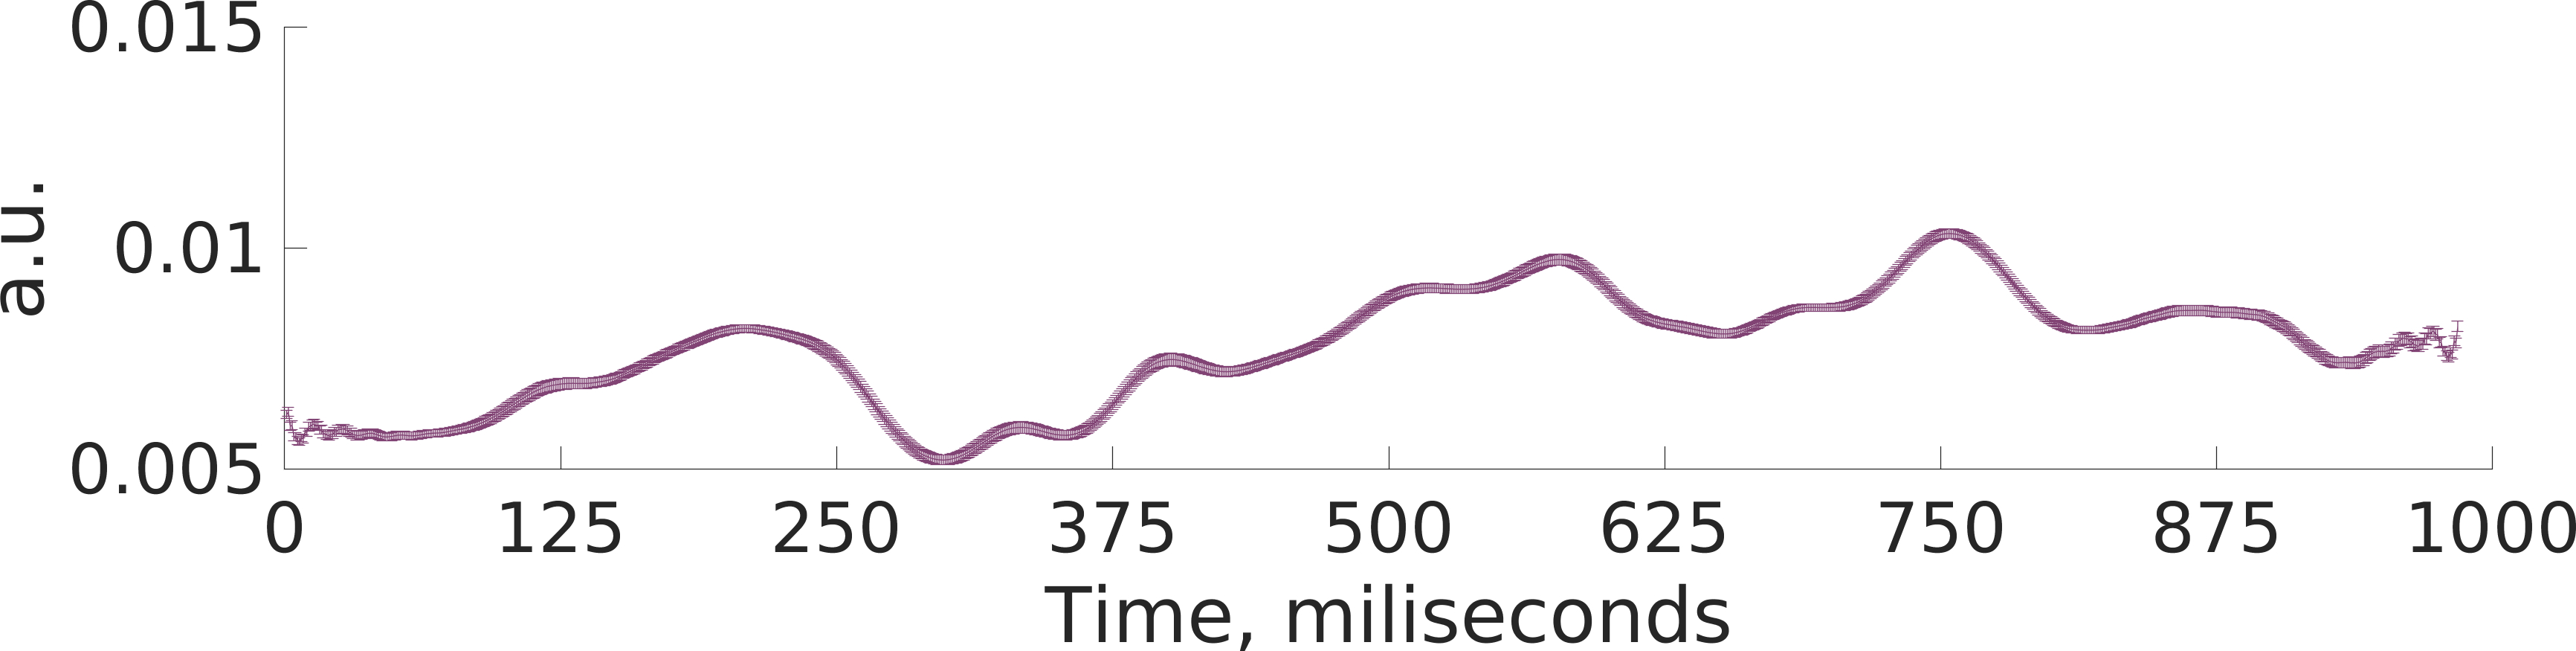
\includegraphics[width=\textwidth]{../images/psiicos_paper/Figure13_c2.jpg}
 \caption{Ниж. гамма-диапазон, Im, сеть 1}\label{fig:13c}
 \end{subfigure}
 \caption{Пространственная структура и временная динамика наиболее воспроизводимых сетей в нижнем (30--60 Гц) и верхнем (65--85 Гц) гамма-диапазонах}\label{fig:13}
\end{figure} % Figure 13

Сети, найденные по мнимой части кросс-спектра, включают связь в альфа-диапазоне
билатеральных сенсорных областей со срединной внутренней поверхностью
коры,~\ref{fig:11b}, а также кросс-латеральные связи между относящимися к руке
зонами сенсорной коры в бета-диапазоне,~\ref{fig:12c}.

Мы также сравнили результаты нашего анализа коннективности с
пространственно-специфичным распределением индуцированной мощности по
коре,~\ref{appendix:real_data_power}. Результаты этого сравнения показывают,
что все обнаруженные сети кроме одной билатеральной сети в бета-диапазоне не
демонстрируют ситуации, когда оба узла сети лежат в областях с высокой
мощностью. В то же время, сенсомоторная область правого полушария, будучи узлом
большинства найденных сетей, совпадает с областью наибольшей активации. Так как
правая сенсомоторная кора играет ключевую роль в исходном
исследовании~\cite{DeLange2008} и так как мы оценивали коннективность не для
одной точки с остальными частями коры, а всех точек со всеми, мы находим эти
результаты обнадеживающими.

\section{Действие проекции на компоненты кросс-спектра в пространстве источников.}\label{sec:subspaces_attenuation}

Из-за ортогональности 2-топографий действительной и мнимой частей операция
проекции никак не влияет на мнимую часть кросс-спектра. На действительную
часть, содержащую информацию о малых фазовых задержках, проекция напротив
оказывает значительное влияние.  Удаляя часть, соответствующую протечке
сигнала, мы неизбежно удаляем и часть полезного сигнала. Качество работы
предложенного алгоритма подавления протечки сигнала в действительной части
кросс-спектра существенно зависит от следующих двух факторов:

\begin{itemize}
    \item PSIICOS-проекция должна максимально подавлять мощность компонент в
        подпространстве протечки сигнала и одновременно с этим минимально
        изменять мощность истинной действительной части когеренции.
    \item Как и для всех алгоритмов решения обратной задачи PSIICOS-проекция
        существенно зависит от точности прямой модели. Неизбежная погрешность
        при ее построении~\cite{Mosher1999} оказывает соответствующее влияние
        на качество решений предложенного метода. Вместе с тем, ошибки прямой
        модели в разумных пределах должны вызывать лишь незначительное
        ухудшение качества решения.
\end{itemize}

Степень выполнения этих условий зависит от феноменологических характеристик
массива сенсоров, а также от магнитных топографий имеющихся мозговых
источников. В этом разделе мы опишем результаты численного моделирования,
направленного на изучение этой проблемы.

Подавление мощности в подпространстве действительной части кросс-спектра
очевидным образом проявляется наиболее сильно для источников с коррелированными
топографиями.  Для исследования зависимости подавления от коэффициента
корреляции между топографиями взаимодействующих источников для каждой пары
индексов $i, j$ мы вычисляли нормы до и после проекции для 2-топографий вида
$\vec{g}_i \otimes \vec{g}_i + \vec{g}_j \otimes \vec{g}_j$,
$\vec{g}_j\otimes\vec{g}_i + \vec{g}_i\otimes\vec{g}_j$ а также
$\vec{g}_j\otimes\vec{g}_i - \vec{g}_i\otimes\vec{g}_j$, соответствующие
подпространствам $S^{SL}, S^{\Im}, S^{\Re}$. Результаты представлены на графике~\ref{fig:02}.

\begin{figure}[!ht]
 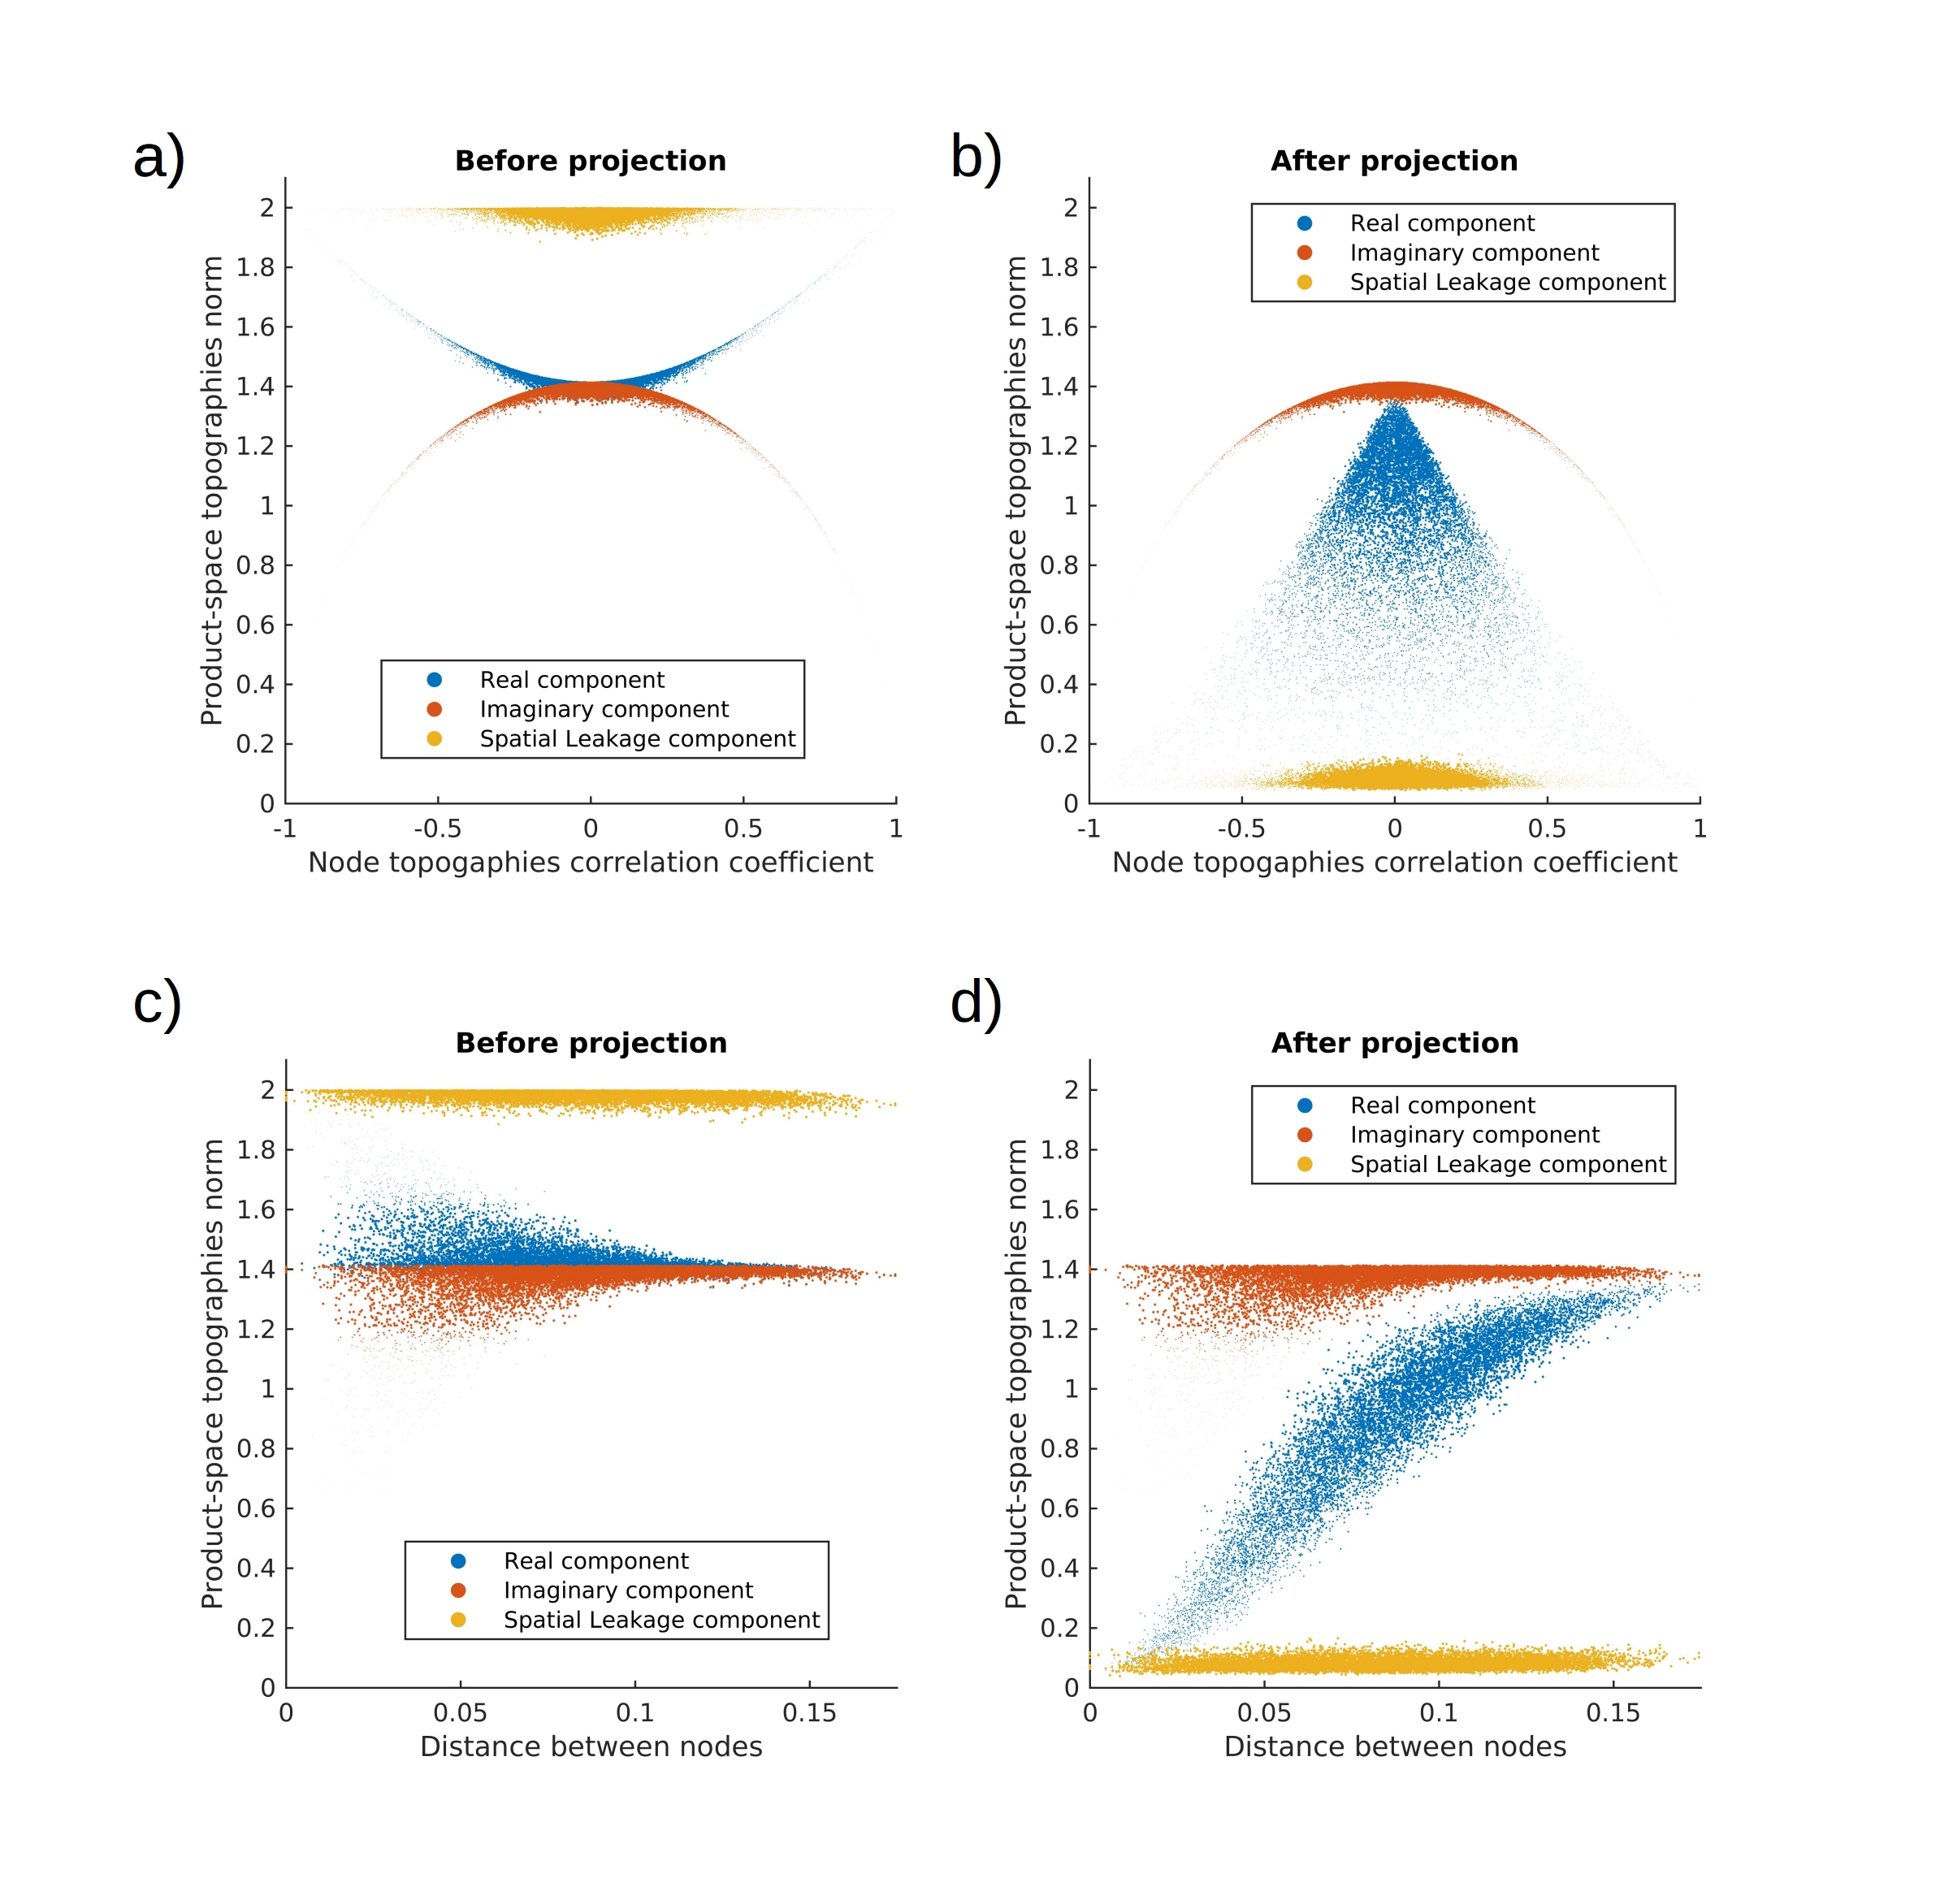
\includegraphics[width=1\textwidth]{../images/psiicos_paper/Figure3abcd_hr}
 \caption{Нормы 2-топографий для трех подпространств кросс-спектра до и после проекции
     в зависимости от коэффициента корреляции топографий взаимодействующих
     узлов на коре (графики (a) и (b)), а также от расстояния между
     этими узлами (графики (c) и (d)).}\label{fig:02} % Figure 3 in the text
     До проекции (графики (a), (c)) в кросс-спектр на уровне сенсоров наибольший вклад дает мощностная
     компонента (обозначена желтым цветом). После проекции (графики (b), (d))
     вклад мощностной компоненты уменьшается в среднем в 25 раз. Вместе с
     тем наблюдается неизбежное, но значительно меньшее ослабление
     2-топографий действительной части, соответствующих истинной коннективности.
     В среднем они ослабляются в 1.6 раз.
\end{figure}

Для каждой сети с узлами в точках $i$ и $j$ на коре соответствует три точки
разных цветов на графике: красная, синяя и желтая. Градации синего цвета мы
использовали для кодировки информации о величине нормы 2-топографии
действительной части $\vec{g}_j\otimes\vec{g}_i + \vec{g}_i\otimes\vec{g}_j$.
Градации красного цвета использовались для 2-топографий мнимой части, и
желтого~--- для топографий протечки сигнала.  Положение каждой цветной точки
вдоль оси $x$ для панелей (a), (b) определялось величиной коэффициента
корреляции топографий $\vec{g}_i$ и $\vec{g}_j$.  Кроме того, мы отобразили те
же самые данные на втором графике, где вместо корреляции по оси $x$
использовалось расстояние между узлами сети $i, j$. Насыщенность цвета точек
отражает плотность точек в соответствующей области графика.

\section{Выбор ранга проекции}\label{subsec:rank_impact}

Мы изучили зависимость коэффициентов ослабления подпространствах протечки
сигнала, а также мнимой и действительной части в зависимости от ранга проекции.
На рисунке~\ref{fig:14} показано среднее затухание мощности в трех
подпространствах в зависимости от ранга проекции.

На практике для ускорения расчетов при обработке МЭГ-данных часто пользуются
методом главных компонент для сокращения размерности пространства сенсоров.
Различные кривые на графике показывают, каким образом ведет себя PSIICOS-проекция
для разных рангов при таком сокращении размерности.

Чтобы получить этот график, мы использовали симуляции Монте-Карло.
На каждой итерации мы случайным образом выбирали подмножество из 200 источников
и вычисляли все 2-топографии из трех подпространств $S_{SL}, S_{\Re}, S_{\Im}$.
Мы использовали источники с фиксированными ориентациями, ортогональными к поверхности коры.
Затем мы изменяли ранг проекции и вычисляли спроецированные версии 2-топографий этих сетей.
Для количественной оценки эффекта затухания мы рассчитывали среднее отношение
норм исходных и спроецированных 2-топографий для каждого значения ранга проекции.
Этот процесс мы повторили 100 раз и усреднили результат.

Из-за пересечения подпространств $S_{SL}$ и $S_{\Re}$ операция проецирования
стремится подавить мощность компоненты SL, что неизбежно приводит к подавлению
мощности в подпространстве $S_{\Re}$.  Чем меньше мощность в подпространстве
$S_{\Re}$ подавляется для фиксированного коэффициента подавления мощности в
$S_{SL}$, тем выше итоговое качество решения. Поэтому в дополнение к кривым
затухания для подпространств мы также нанесли логарифм отношения коэффициентов
ослабления, наблюдаемых для векторов в подпространстве $S_{\Re}$, к векторам в
подпространстве $S_{SL}$. Использование SVD-разложения при формировании
оператора проекции делает возможным значительно более быстрое уменьшение
мощности в подпространстве протечки сигнала $S_{SL}$, чем в подпространстве $
S_{\Re}$. Другими словами мы видим, что увеличение ранга проекции приводит к
все большему доминированию мощности в подпространстве $S_{\Re}$ по сравнению с
подпространством $S_{SL}$.

\begin{figure}[htbp]
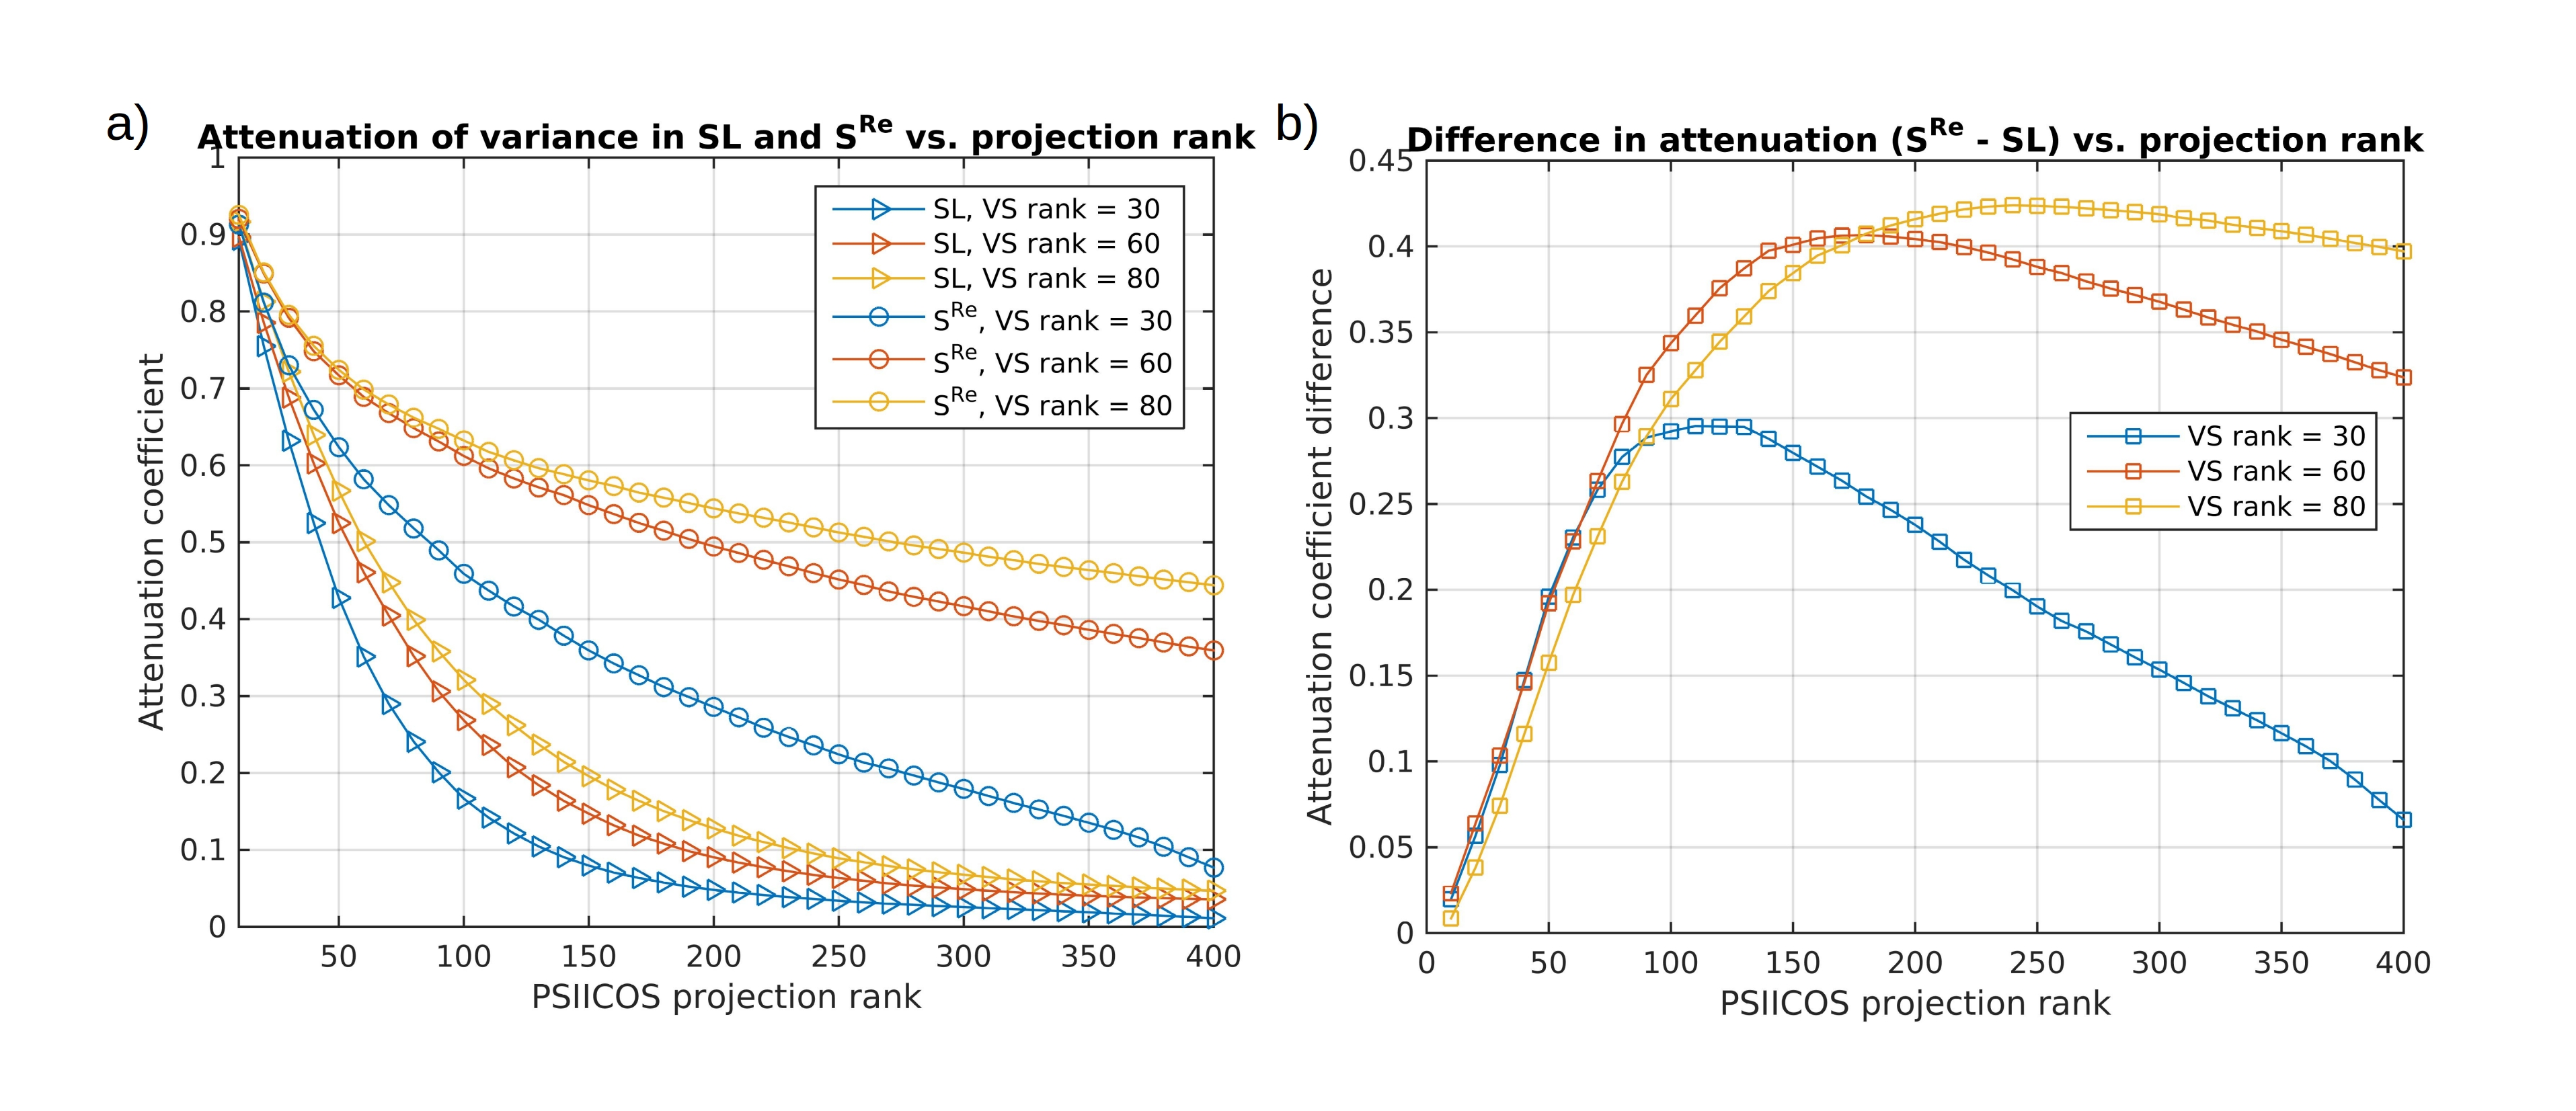
\includegraphics[width=\textwidth]{../images/psiicos_paper/Figure14_hr.jpg}
\caption{(a) Ослабление мощности в подпространствах $S_{SL}$ и $S_{Re}$ и (b)
    Разница в коэффициенте затухания для подпространств $S_{Re}$ и $S_{SL}$ как
    функции ранга проекции для трех различных размерностей пространства виртуальных
    сенсоров (VS).
}\label{fig:14}
    Эти кривые позволяют принять обоснованное решение
    относительно выбора ранга проекции.  Мы предлагаем выбирать такое значение ранга
    проекции PSIICOS, которое соответствует наибольшей разнице в затухании
    мощности.
\end{figure}

\section{Влияние неточностей прямой модели на качество решений}\label{sec:forward_model_errors_effect}

Описанная проекция строится на основании прямой модели, которая в реальных
условиях неизбежно содержит к неточностям.  В этом разделе мы изучили
эффективность предложенной операции проецирования при наличии структурированных
и неструктурированных ошибок в прямой модели.

В этом исследовании мы использовали две различные модели шума.  Первая модель
соответствовала пространственно неструктурированному шуму и была реализована
путем добавления масштабированного случайного шума к матрице прямой модели.

Чтобы получить матрицу реализации шума при оценке прямой модели, мы
семплировали данные из стандартного нормального распределения $N(0,1)$.  Далее
мы нормировали эти данные умножением элементов матрицы шума на квадратный корень
из среднего значения следа матрицы $\matr{G}\matr{G}^T$, где
$\matr{G}$~--- матрица прямой модели. Затем мы добавляли эту матрицу к
истинной прямой модели и корректировали количество шума с помощью
параметра $\alpha$.

Вторая модель соответствовала более реалистичному сценарию пространственно
структурированного искажения.  Для генерации пространственно структурированной
шумовой матрицы мы использовали модели головы, рассчитанные для $N=10$
испытуемых, и посчитали разницу между прямыми моделями для каждой пары
субъектов. Мы вычисляли матрицу структурированного шума как среднее из этих
попарных разниц. Затем мы нормировали полученную матрицу структурированного
шума и добавляли ее к истинной прямой модели. Как и в предыдущем случае, мы
регулировали количество шума с помощью параметра $\alpha$.

Потенциально неточности прямой модели могут привести к одновременному
уменьшению ослабления мощности подпространства протечки сигнала и уменьшению
мощности подпространства $S_{\Re}$.  Мы использовали симуляции Монте-Карло для
численного изучения этих эффектов.  На каждой итерации мы случайным образом
выбирали подмножество из 200 источников и рассчитывали средний коэффициент
ослабления для трех подпространств.  Мы сделали это как для случая
структурированного, так и для неструктурированного шума, а также для двух разных
значений ранга проекции (350 и 500). Результаты представлены на рисунке~\ref{fig:15}.

Мы можем видеть, что хотя неточности в прямой модели приводят к
ухудшению работы предлагаемого метода проекции, для типичных уровней
шума в прямой модели для MEG порядка 10 \% (\cite{Mosher1999}) мы имеем почти одинаковое значение
подавления мощности в подпространстве протечки сигнала и только около 20 \% дополнительного уменьшения мощности
в подпространстве $S_{\Re}$.

\begin{figure}[htbp]
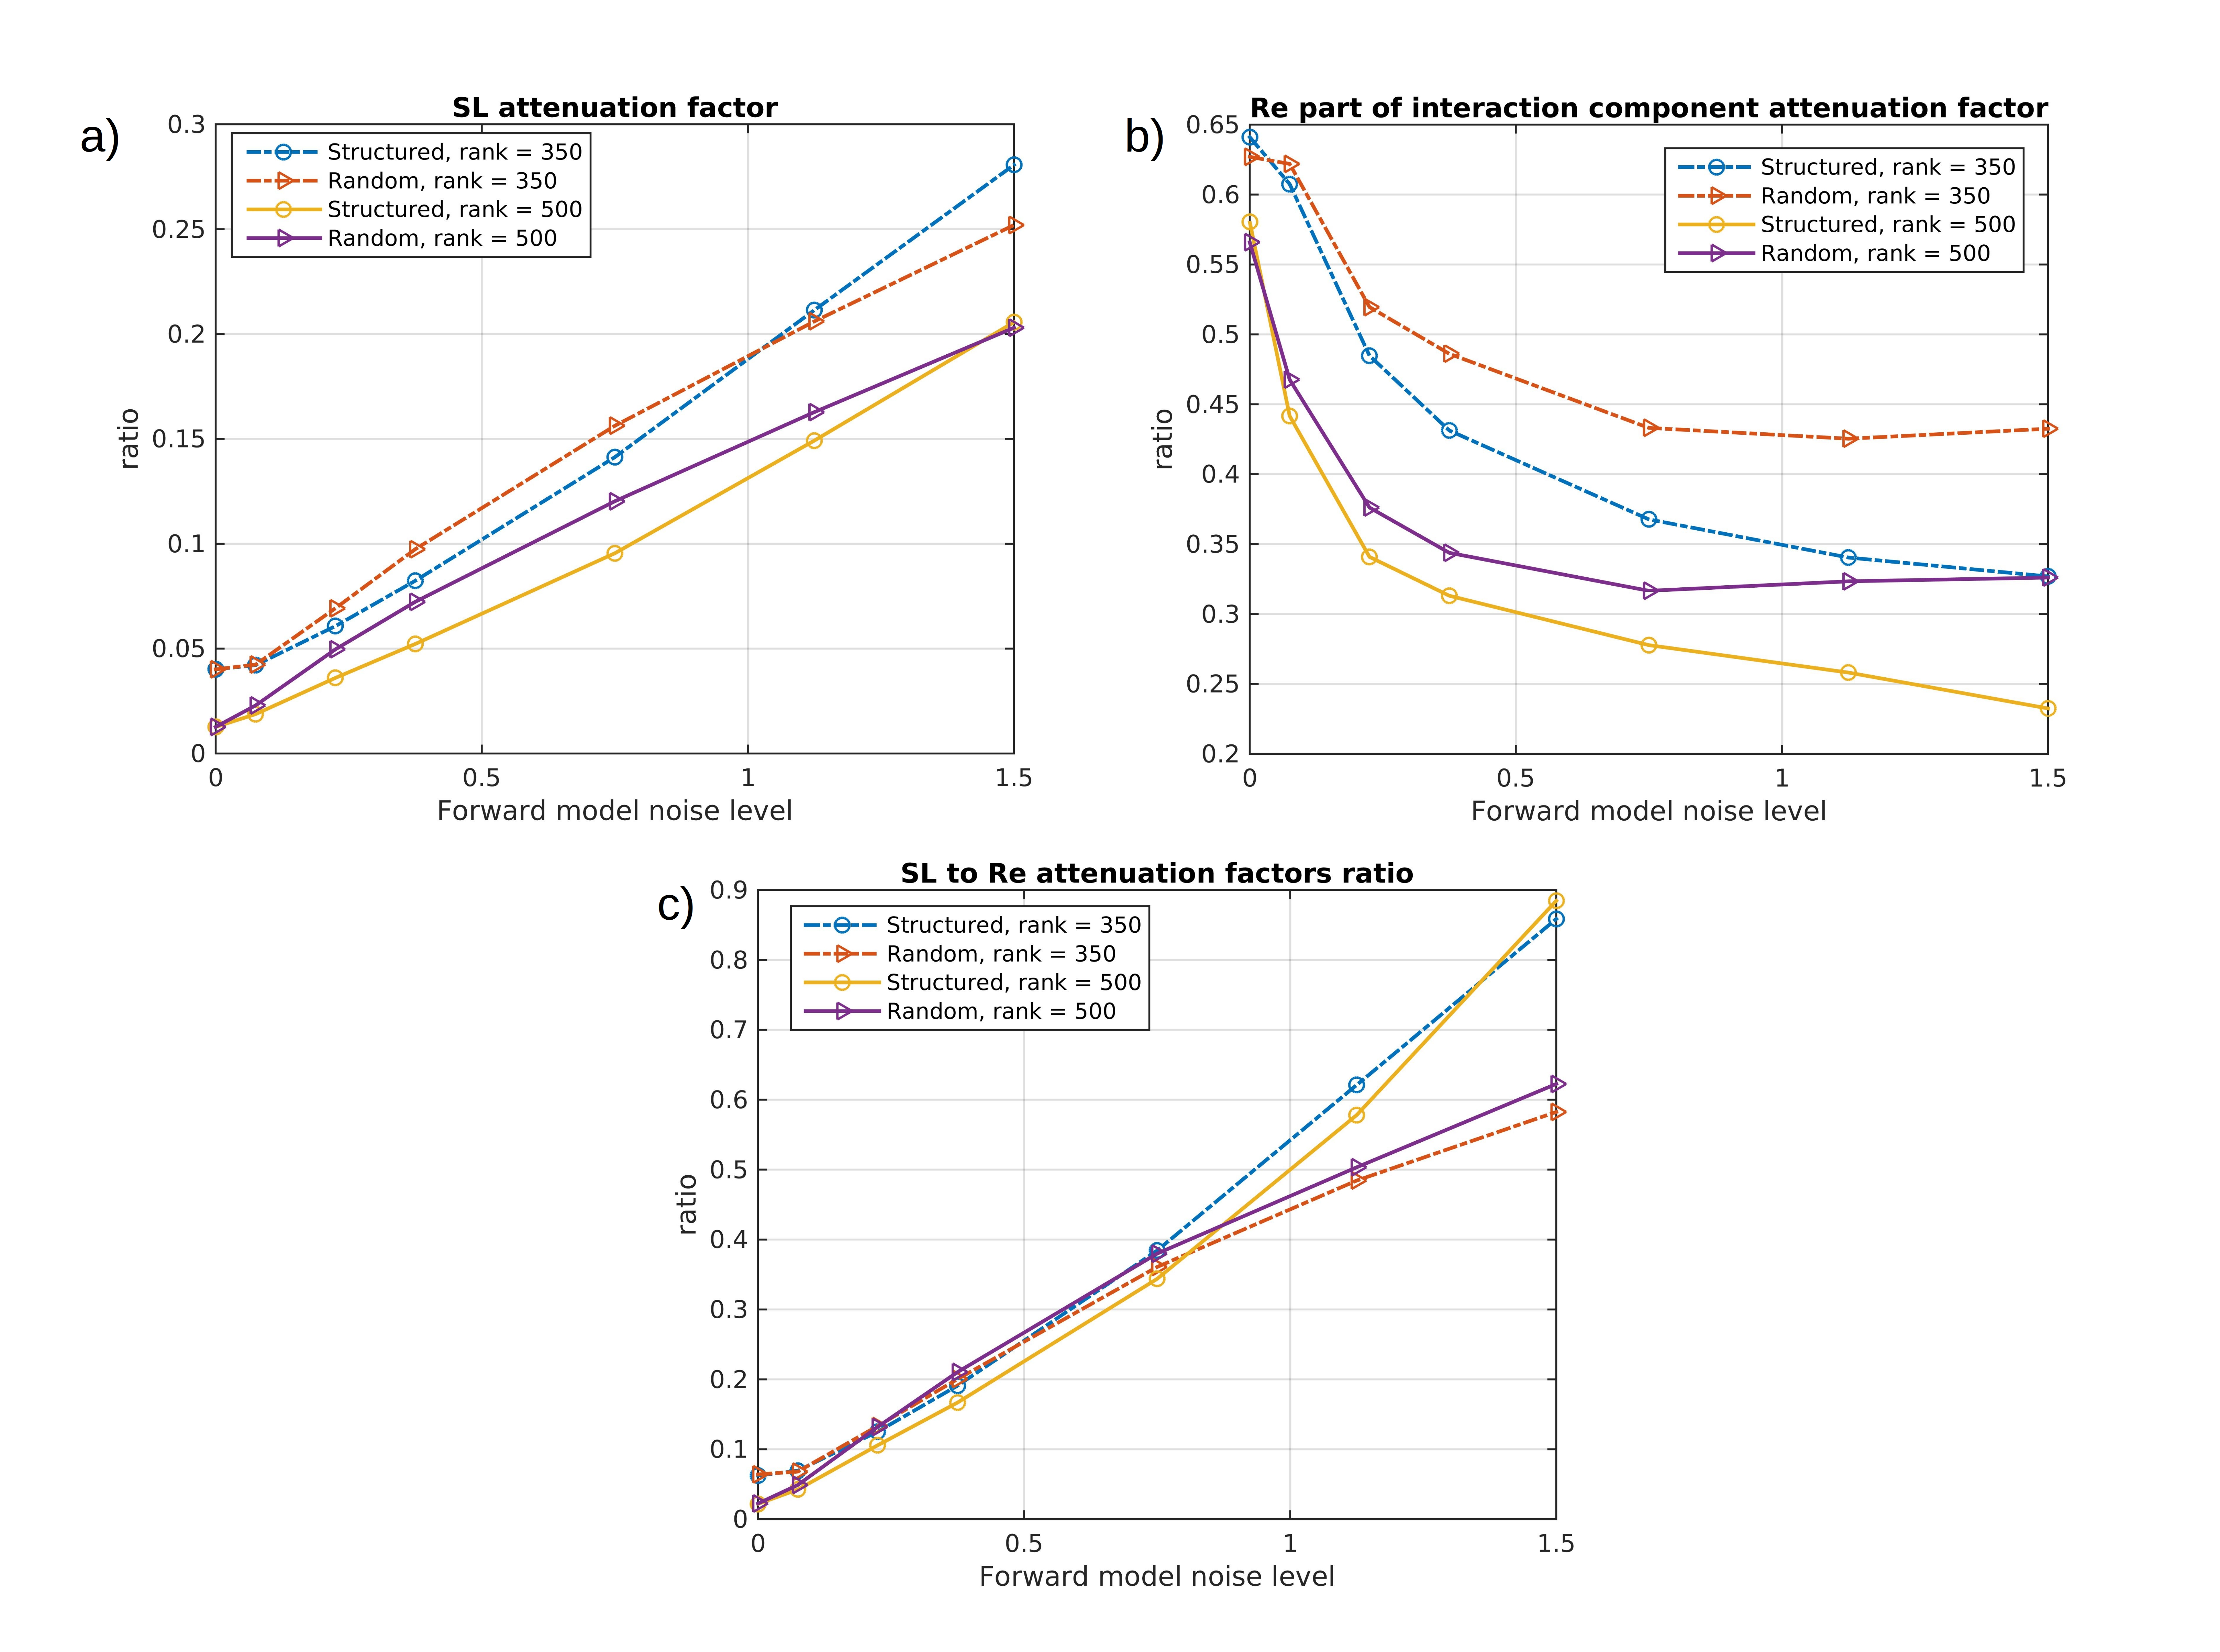
\includegraphics[width=1\textwidth]{../images/psiicos_paper/Figure15_hr.jpg}
\caption{Влияние шума в прямой модели на качество проекции.}\label{fig:15} %Figure 15
  На панели (a) изображена зависимость коэффициента затухания от интенсивности шума $\alpha$.
  Панель (b) показывает коэффициент ослабления мощности в подпространстве $S_{\Re}$.
  На панели (с) нарисовано подавление мощности в подпространстве SL по сравнению с мощностью в $S_{\Re}$.
  Как видим, оно монотонно убывает с ростом интенсивности шума в прямой модели.
 \end{figure}

Из-за пересечения подпространств $S_{SL}$ и $S_{\Re} $ при попытке
подавить компоненту протечки сигнала, алгоритм также подавляет мощность в
подпространстве истинного взаимодействия $S_{\Re}$. Неточности в прямой модели
увеличивают нежелательное подавление мощности в подпространстве $S_{\Re} $ и уменьшают
эффективность подавления мощности в подпространстве протечки сигнала.
Такое ухудшение производительности с увеличением погрешности в прямой модели
можно охарактеризовать соотношением коэффициентов затухания 2-топографий в подпространствах $S_{SL}$ и $S_{\Re}$.
Когда это соотношение меньше единицы, мы можем сказать, что мощность в подпространстве $S_{SL}$
уменьшилась сильнее, чем мощность в подпространстве $ S_{\Re}$. Следовательно
чем меньше это соотношение, тем лучше производительность предлагаемой схемы.

На панели (c) рисунка~\ref{fig:15} мы отобразили соотношение коэффициентов ослабления мощности в подпространствах
$S_{SL}$ и $ S_{\Re}$. Как мы видим, значение этого отношения плавно меняется с
ростом интенсивности шума в прямой модели и остается низким для уровня шума 10 \%.

На основании представленных численных результатов мы можем заключить, что метод
является достаточно надежным для типичных уровней шума в прямой модели и может
использоваться в реальных условиях.  Однако, как и во многих других методах,
использующих прямую модель (например,~\ref{subsec:DICS}), усилия, направленные на
получение более точных прямых моделей способны принести ощутимую отдачу и ими
не следует пренебрегать.



\section{Сравнение стратегий нормализации весов фильтра для метода PSIICOS.}
Как мы уже отмечали в разделе~\ref{subsec:psiicos_normalization_and_spatial_bias},
базовая процедура оценки кросс-спектральных коэффициентов (см.
раздел~\ref{sec:psiicos}) в пространстве источников дает пространственно смещенную оценку.
В разделе~\ref{subsec:psiicos_normalization_and_spatial_bias} мы предложили модификацию
метода, основанную на другой нормализации весов фильтров по аналогии с методом sLORETA,~\cite{Pascual-Marqui2002}.
В этом разделе мы сравнили качество работы базового алгоритма PSIICOS и модифицированного метода
с теоретически пространственно несмещенной оценкой, который мы будем называть PSIICOS Unbiased.

Для сравнения как и ранее мы использовали симуляции Монте-Карло,
описанные в разделе~\ref{sec:monte_carlo_simulation}, со случайно выбираемыми положениями узлов сети
для каждой итерации процедуры. Как и в предыдущих разделах, качество работы алгоритмов мы сравнивали
на основе ROC-кривых и кривых Precition-Reсall. В этом анализе мы ограничились 100 итерациями Монте-Карло.

Результаты этих симуляций для двух значений фазовой задержки (ОСШ=0.2 и ОСШ=1),
а также для трех значений фазового сдвига, $\phi = \pi/20, \phi = \pi/4$ и $\phi=\pi/2 - \pi/20$,
представлены на рис.~\ref{fig:psiicos_vs_unbiased_monte}.

\begin{figure}[htbp]
    \begin{subfigure}[t]{0.5\textwidth}
        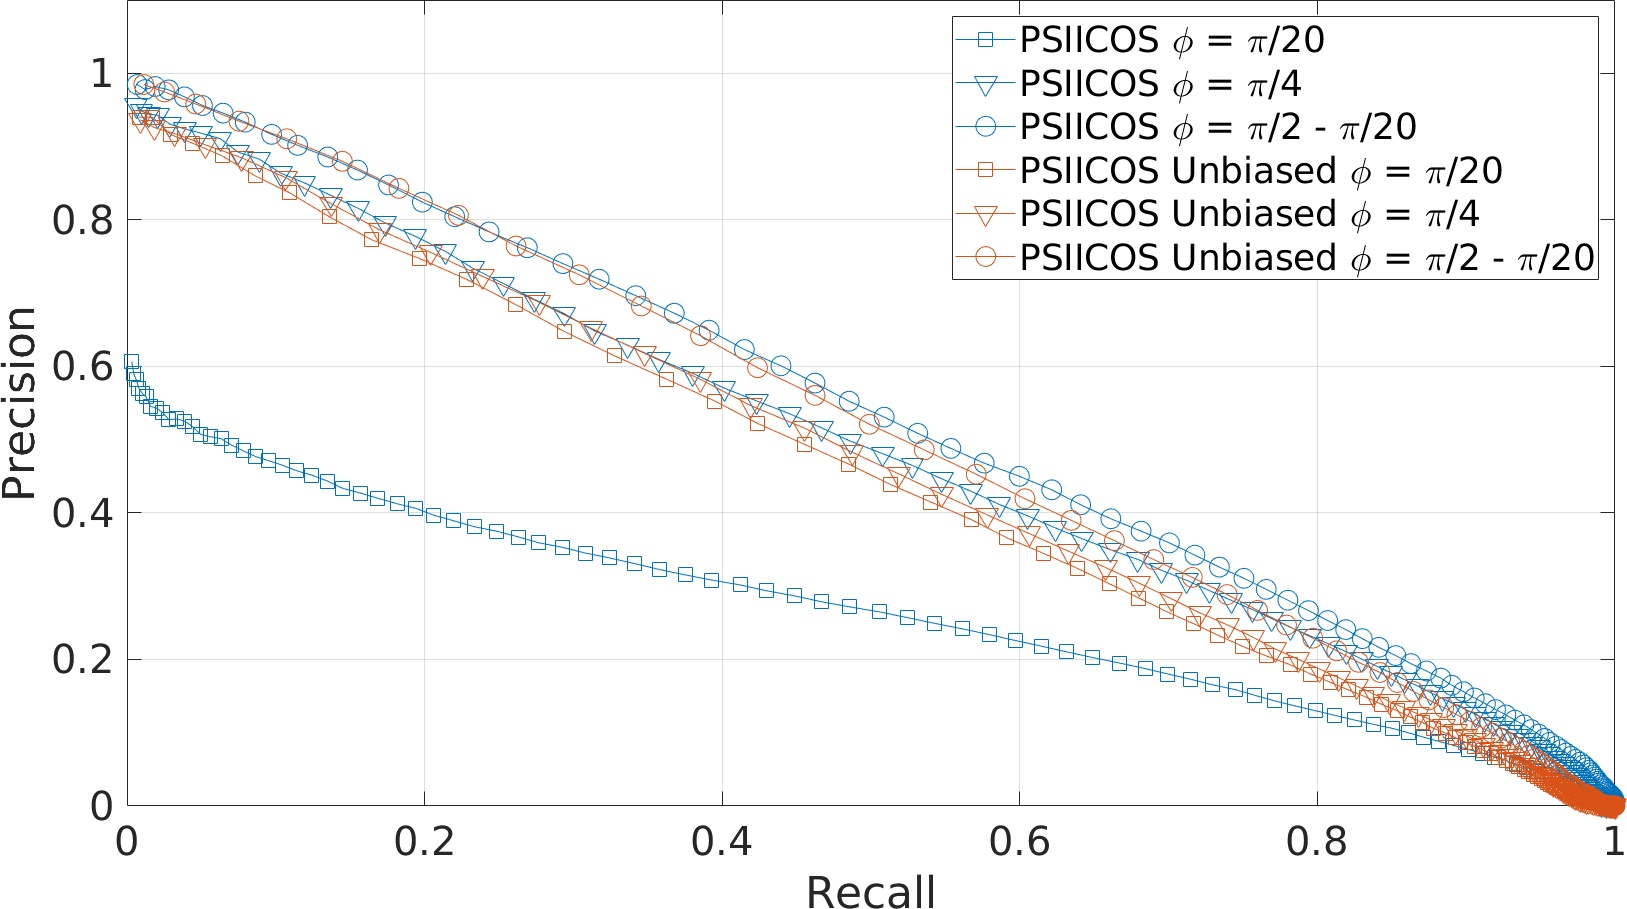
\includegraphics[width=1\textwidth]{../images/pre_rec_snr_1.jpg}
        \caption{Precition-Recall, ОСШ=1}\label{fig:psiicos_vs_unbiased_monte_a}
    \end{subfigure}
        \hspace{-1.5cm}
    \begin{subfigure}[t]{0.5\textwidth}
        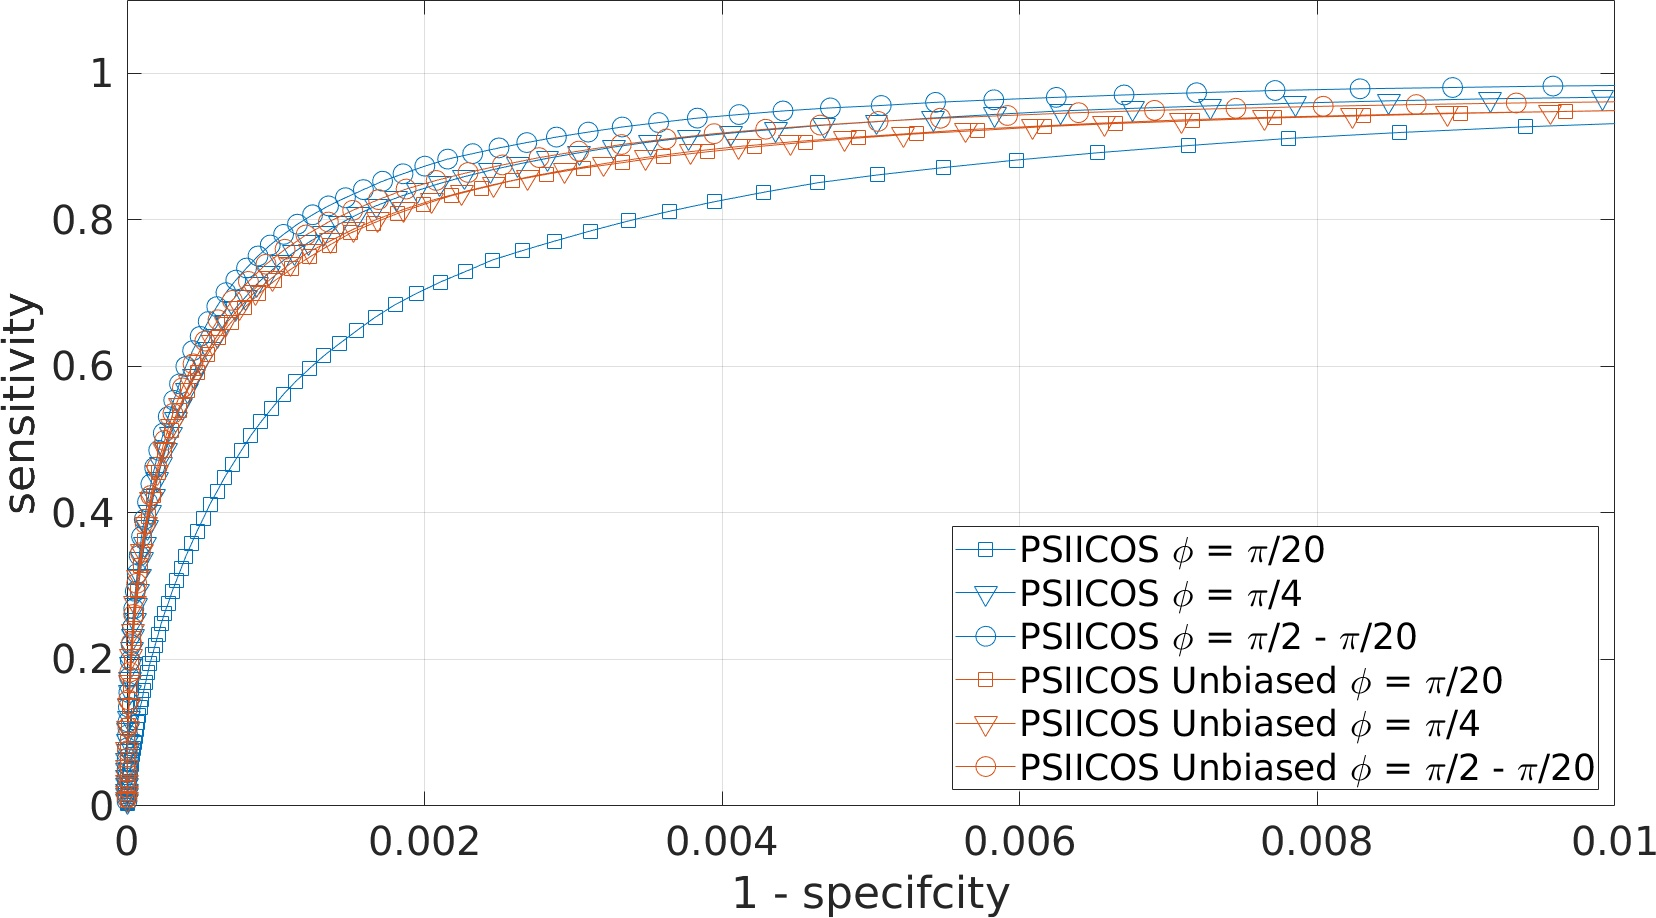
\includegraphics[width=1\textwidth]{../images/roc_snr_1.jpg}
        \caption{ROC, ОСШ=1}\label{fig:psiicos_vs_unbiased_monte_b}
    \end{subfigure}
    \hspace{-2cm}
    \begin{subfigure}[t]{0.5\textwidth}
        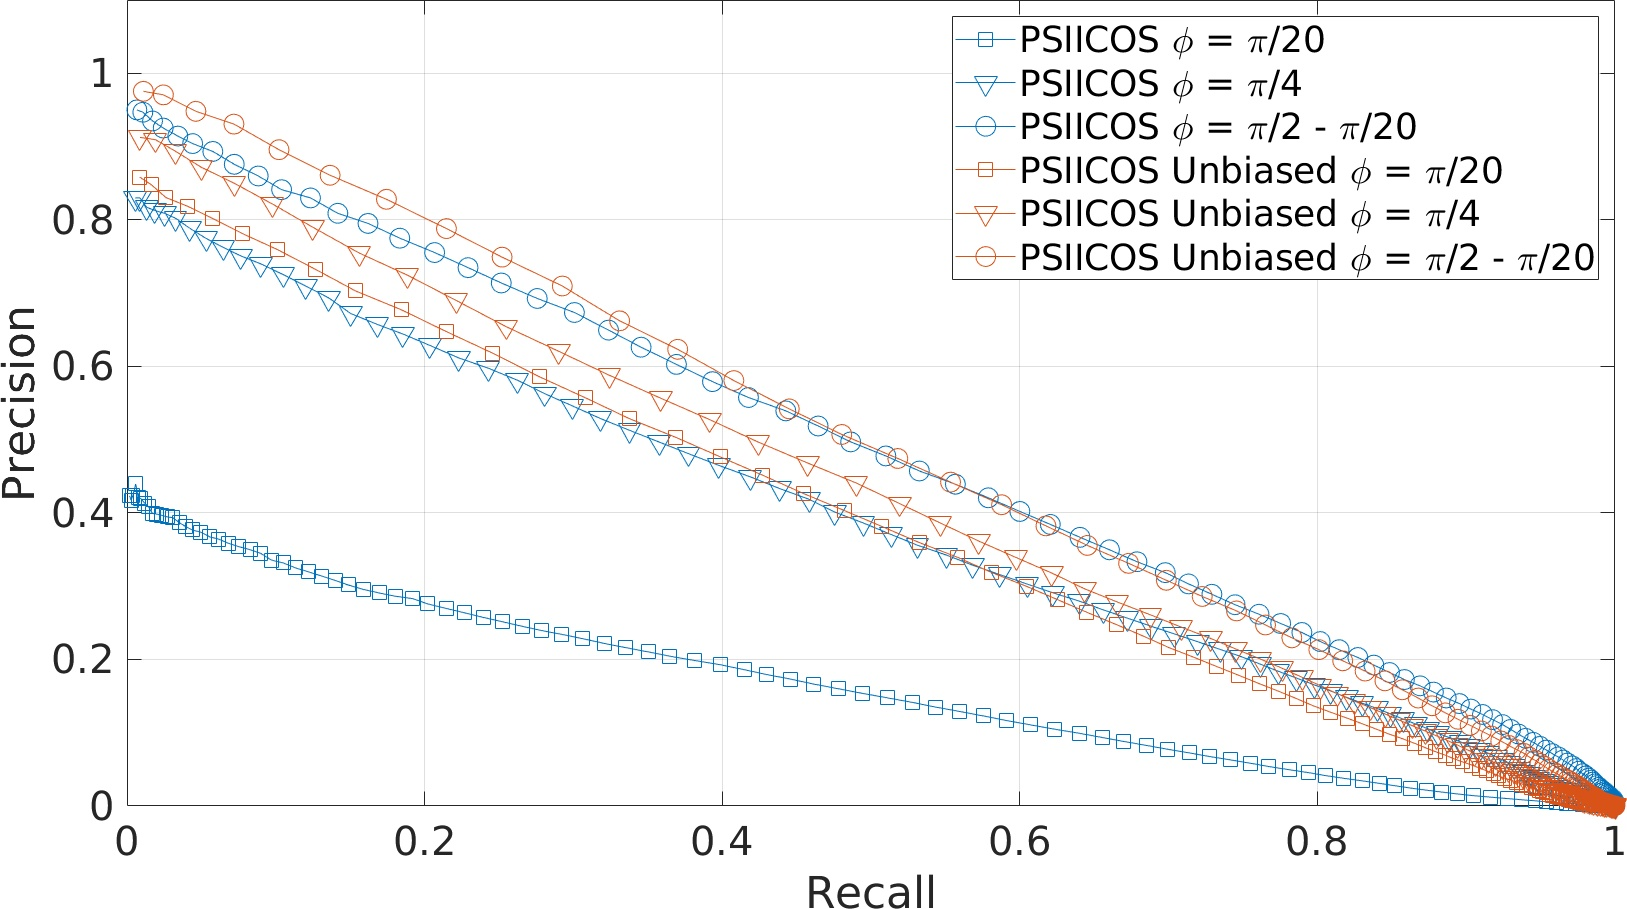
\includegraphics[width=0.99\textwidth]{../images/pre_rec_snr_02.jpg}
        \caption{Precition-Recall, ОСШ=0.2}\label{fig:psiicos_vs_unbiased_monte_c}
    \end{subfigure}
    \begin{subfigure}[t]{0.5\textwidth}
        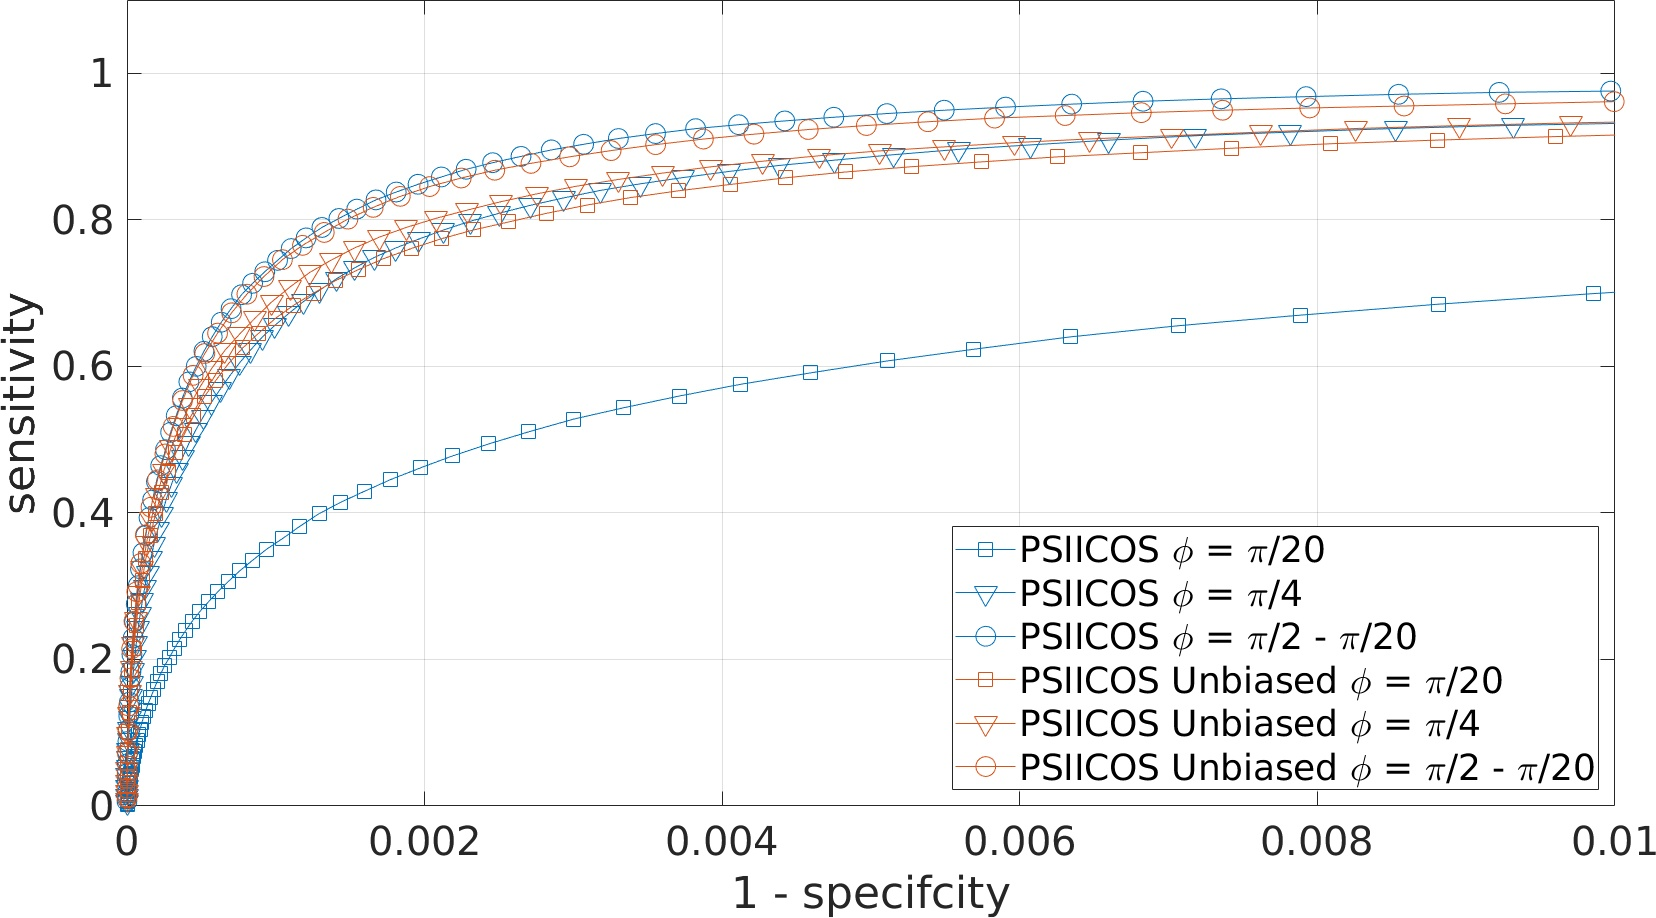
\includegraphics[width=0.99\linewidth]{../images/roc_snr_02.jpg}
        \caption{ROC, ОСШ=0.2}\label{fig:psiicos_vs_unbiased_monte_d}
    \end{subfigure}
    \caption{Сравнение методов PSIICOS и PSIICOS Unbiased в задаче поиска сетей со случайными
    положениями узлов для 100 итераций Монте-Карло.}\label{fig:psiicos_vs_unbiased_monte}
\end{figure}

Из графика~\ref{fig:psiicos_vs_unbiased_monte} видно, что для малых фазовых задержек
как в случае высокого, так и в случае низкого значения ОСШ, метод PSIICOS Unbiased
показывает значительно лучшие результаты. Для остальных значений фазового сдвига
качество решений обеих версий алгоритма приблизительно одинаковое с небольшим
преимуществом метода PSIICOS Unbiased для низкого ОСШ.

Такое преимущество PSIICOS Unbiased для $\phi=\pi/20$ объясняется тем, что в методе
PSIICOS при нормализации мы не делали поправку на применение оператора проекции, который
не влияет на 2-топографии мнимой части, но может значительно уменьшать норму 2-топографий
действительной. В этой связи пространственная смещенность оценки методом PSIICOS должна
быть наиболее сильно представлена, когда фазовые задержки сетей близки к нулю, что и вызывает
снижение качества детекции для случая $\phi=\pi/20$.

На рисунке~\ref{fig:psiicos_vs_unbiased_case_3dbrain} представлен характерный пример, взятый с одной из итераций Монте-Карло (ОСШ=1 и $\phi=\pi/20$),
когда алгоритм PSIICOS показал плохие результаты
по сравнению с PSIICOS Unbiased. На графике хорошо виден эффект пространственной смещенности
метода PSIICOS для более глубокого источника в случае низкой фазовой задержки.
Похожая картина наблюдалась и в других отдельно взятых итерациях Монте-Карло, в которых
метод PSIICOS показывал плохое качество решения на индивидуальной кривой Precision-Recall.

\begin{figure}[htbp]
    \begin{subfigure}[t]{0.5\textwidth}
        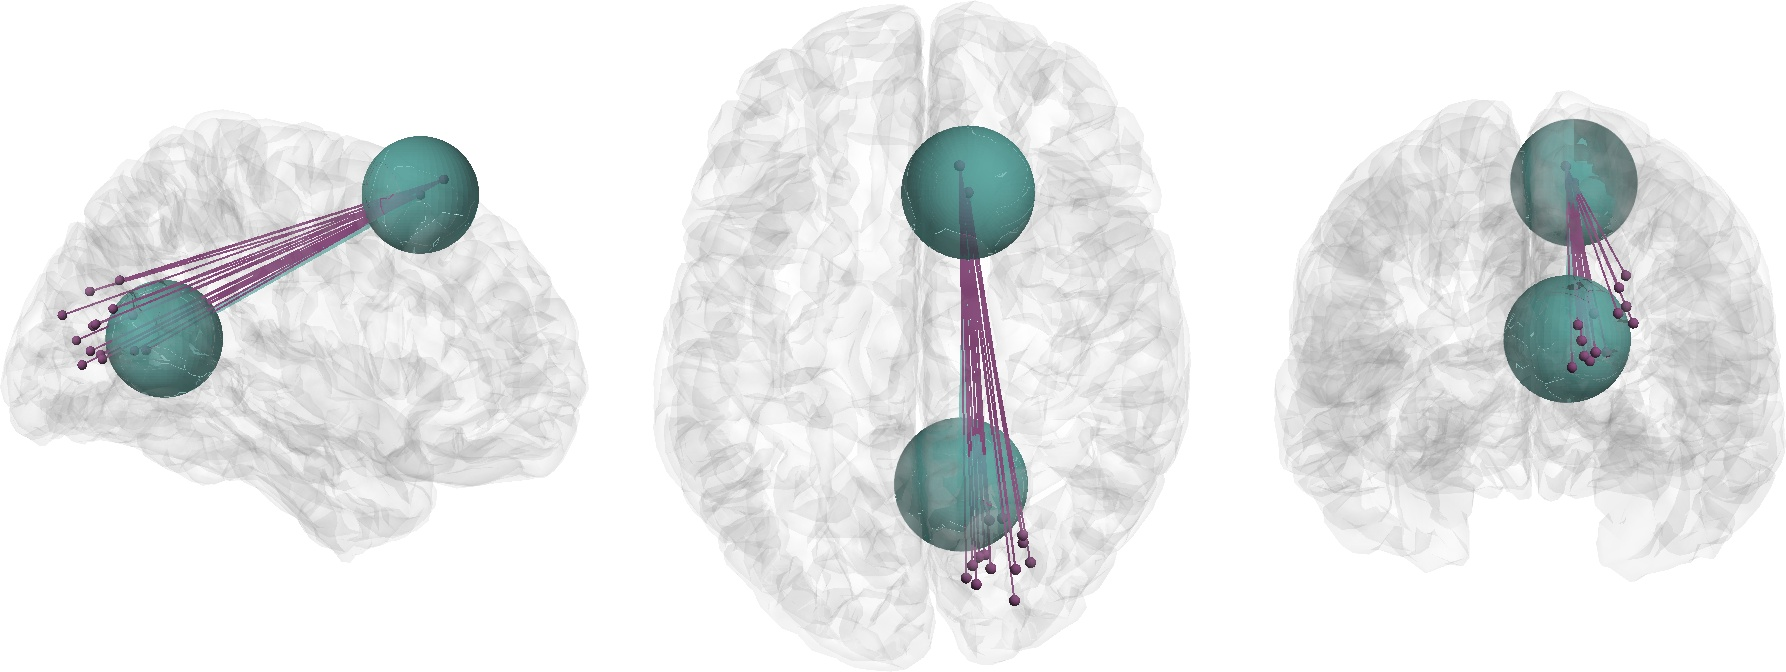
\includegraphics[width=0.99\textwidth]{../images/bias_brain_PSIICOS.jpg}
        \caption{PSIICOS}\label{fig:bias_brain_psiicos}
    \end{subfigure}
    \begin{subfigure}[t]{0.5\textwidth}
        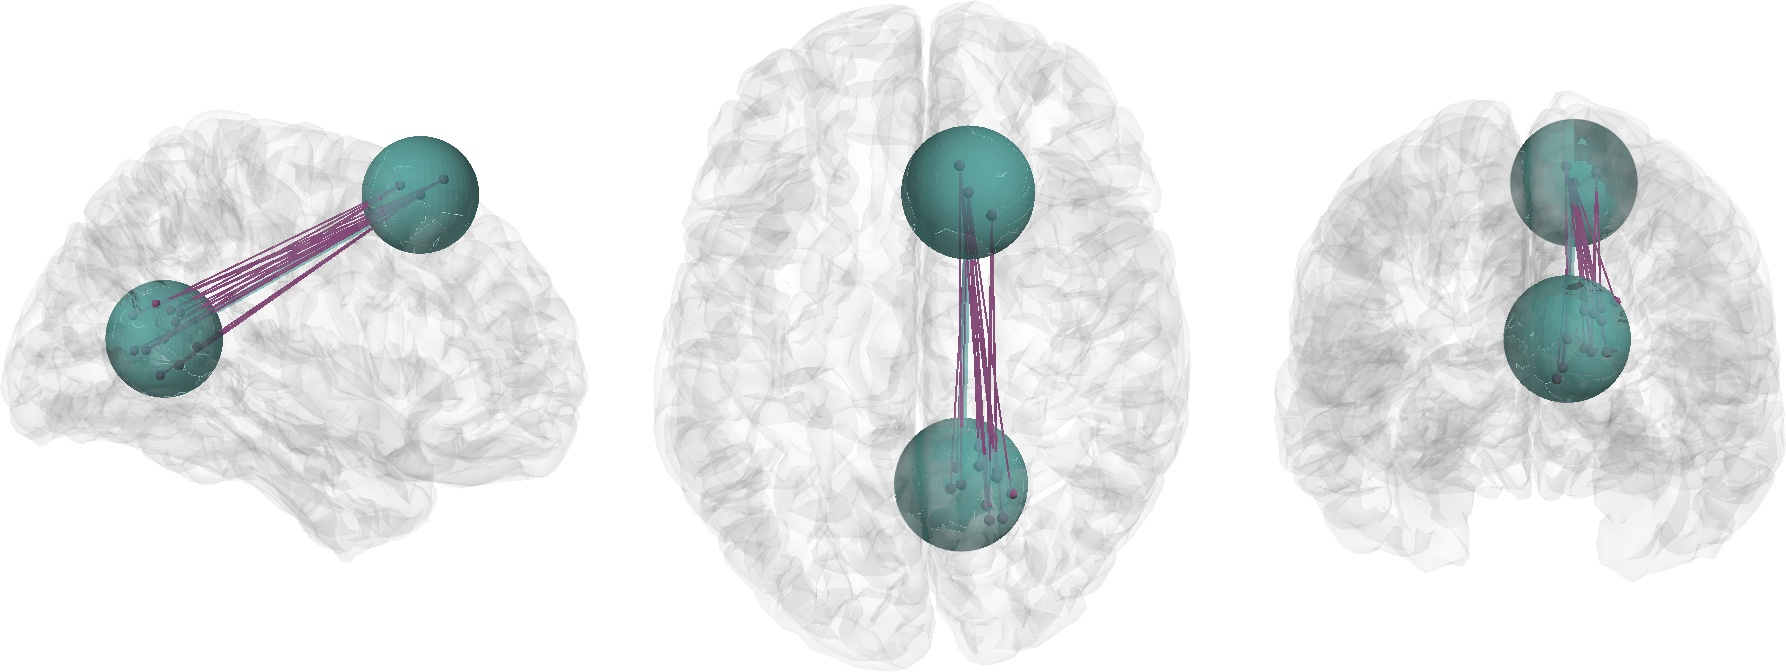
\includegraphics[width=0.99\textwidth]{../images/bias_brain_PSIICOS_Unbiased.jpg}
        \caption{PSIICOS Unbiased}\label{fig:bias_brain_psiicos_unbiased}
    \end{subfigure}
    \caption{Пример плохого решения для алгоритма PSIICOS по сравнению с
        PSIICOS Unbiased в задаче детекции сетей со случайными положениями
        узлов для одной из итераций Монте-Карло и фазового сдвига
        $\phi=\pi/20$.
    }\label{fig:psiicos_vs_unbiased_case_3dbrain}
    Фиолетовые отрезки (по 20 для каждого метода)~--- найденные сети; зелеными
    сферами отмечены зоны, внутри которых найденные сети относились к истинно
    положительным срабатываниям. Радиус каждой сферы равен 1.8 см.
\end{figure}

Далее мы сравнили качество работы двух версий алгоритма PSIICOS в задаче детекции трех
сетей с фиксированными положениями. Пространственная структура и временные профили активации
брались в соответствии с описанием в разделе~\ref{sec:three_ntw}. Как и для сетей со
случайными положениями узлов, мы симулировали сети для двух значений ОСШ и трех
значений фазового сдвига: ОСШ=0.2, ОСШ=1б $\phi=\pi/20, \phi=\pi/4, \phi=\pi/2 - \pi/20$.

Так как в этой симуляции пространственная структура шума мозга случайна
(она задается как 1000 случайно разбросанных по коре генераторов, см.
раздел~\ref{sec:monte_carlo_simulation}), результаты в разных повторениях
этих симуляций несколько отличаются. Чтобы уменьшить влияние этой случайности,
мы усреднили итоговые кривые по 10 повторениям эксперимента.

\begin{figure}[htbp]
    \begin{subfigure}[t]{0.5\textwidth}
        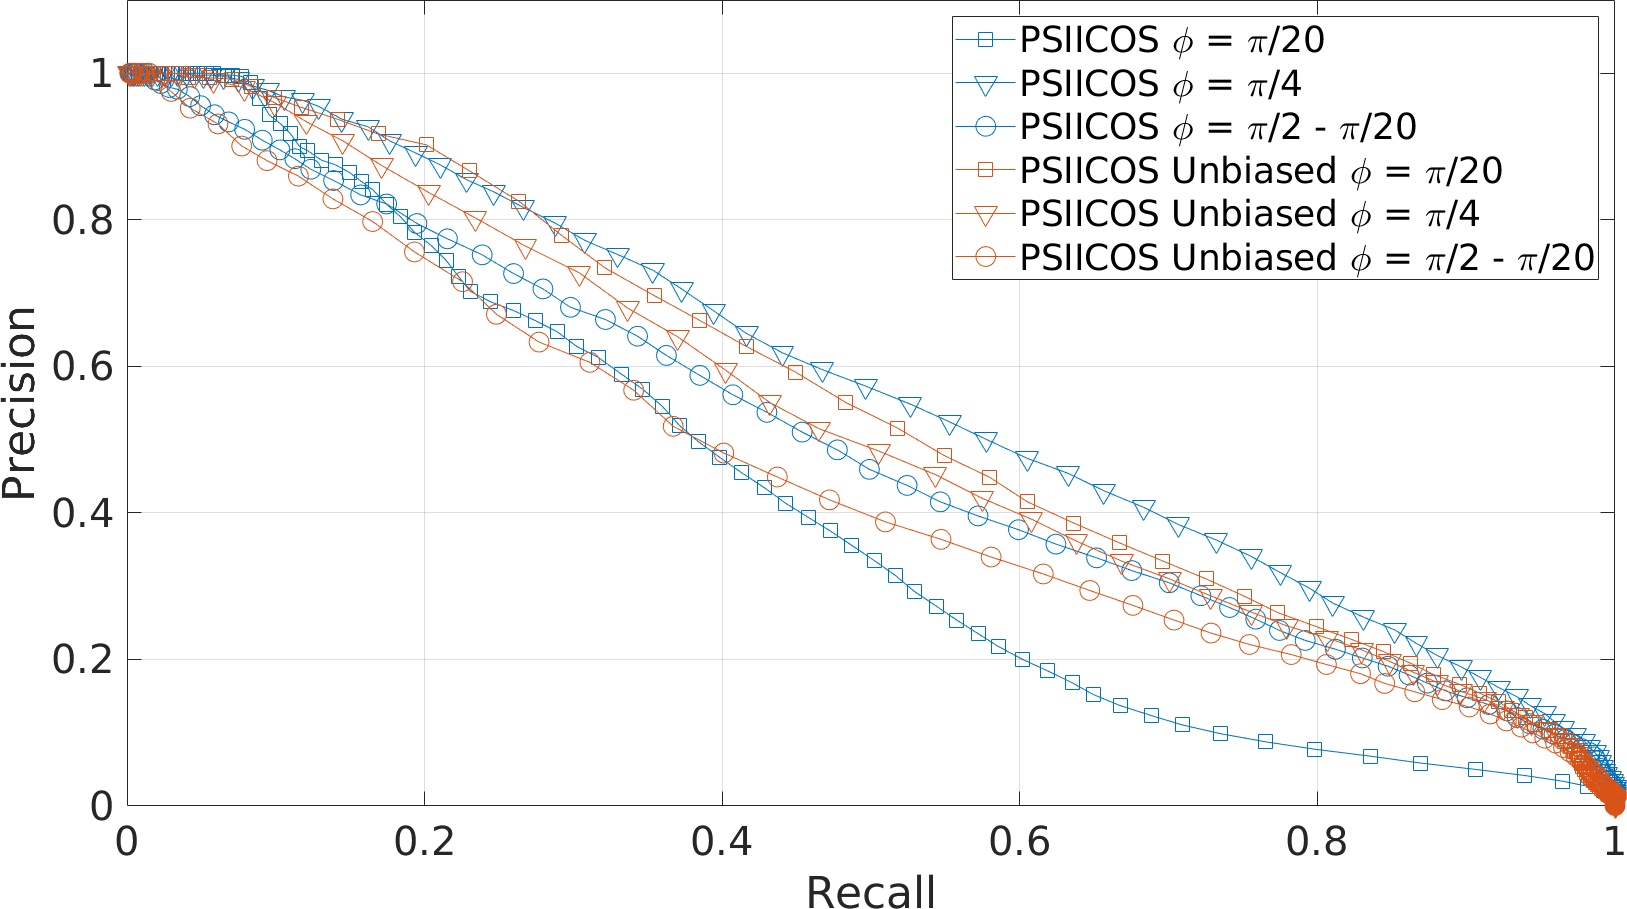
\includegraphics[width=0.99\textwidth]{../images/pre_rec_3_ntw_snr_1.jpg}
        \caption{Precition-Recall, ОСШ=1}\label{fig:psiicos_vs_unbiased_3_ntw_a}
    \end{subfigure}
    \begin{subfigure}[t]{0.5\textwidth}
        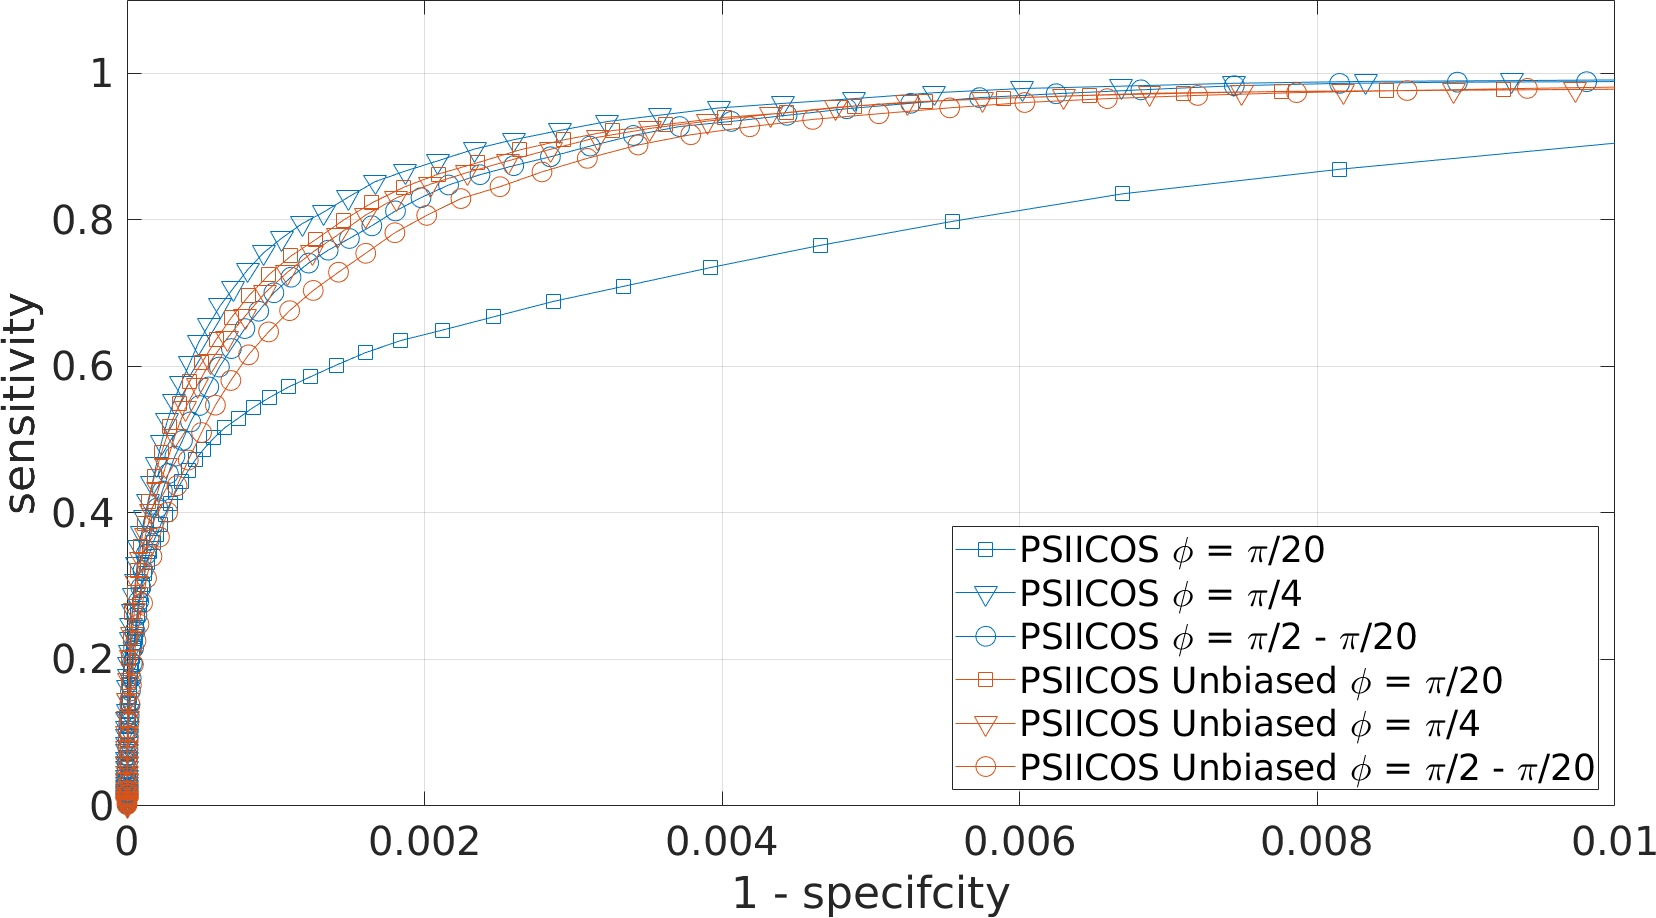
\includegraphics[width=0.99\textwidth]{../images/roc_3_ntw_snr_1.jpg}
        \caption{ROC, ОСШ=1}\label{fig:psiicos_vs_unbiased_3_ntw_b}
    \end{subfigure}
    \begin{subfigure}[t]{0.5\textwidth}
        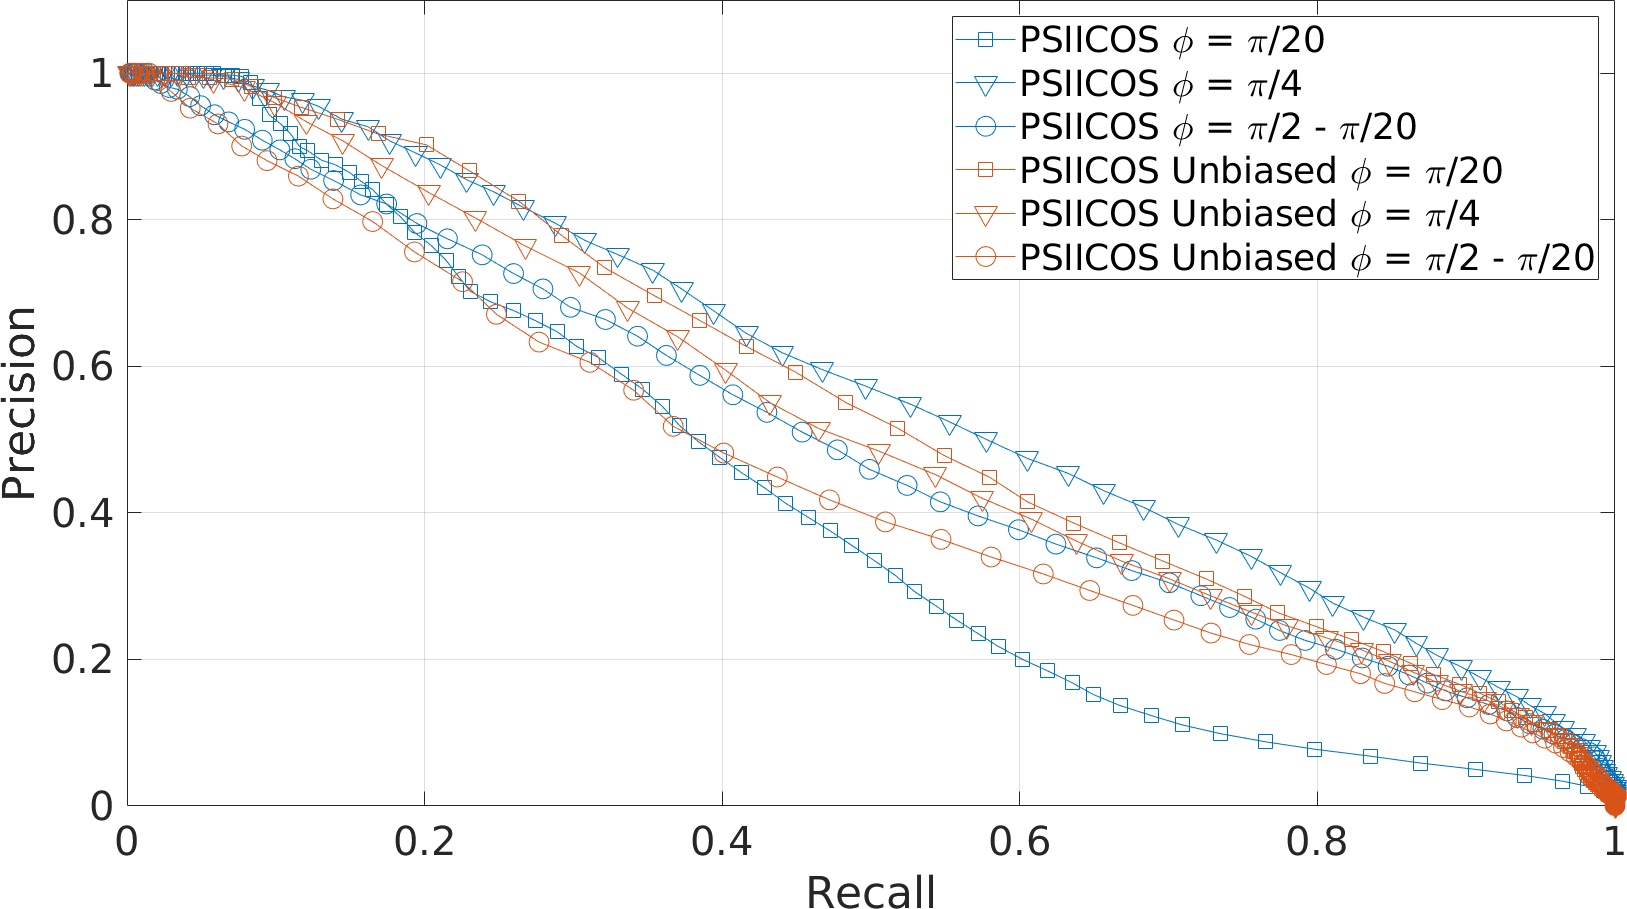
\includegraphics[width=0.99\textwidth]{../images/pre_rec_3_ntw_snr_1.jpg}
        \caption{Precition-Recall, ОСШ=0.2}\label{fig:psiicos_vs_unbiased_3_ntw_c}
    \end{subfigure}
    \begin{subfigure}[t]{0.5\textwidth}
        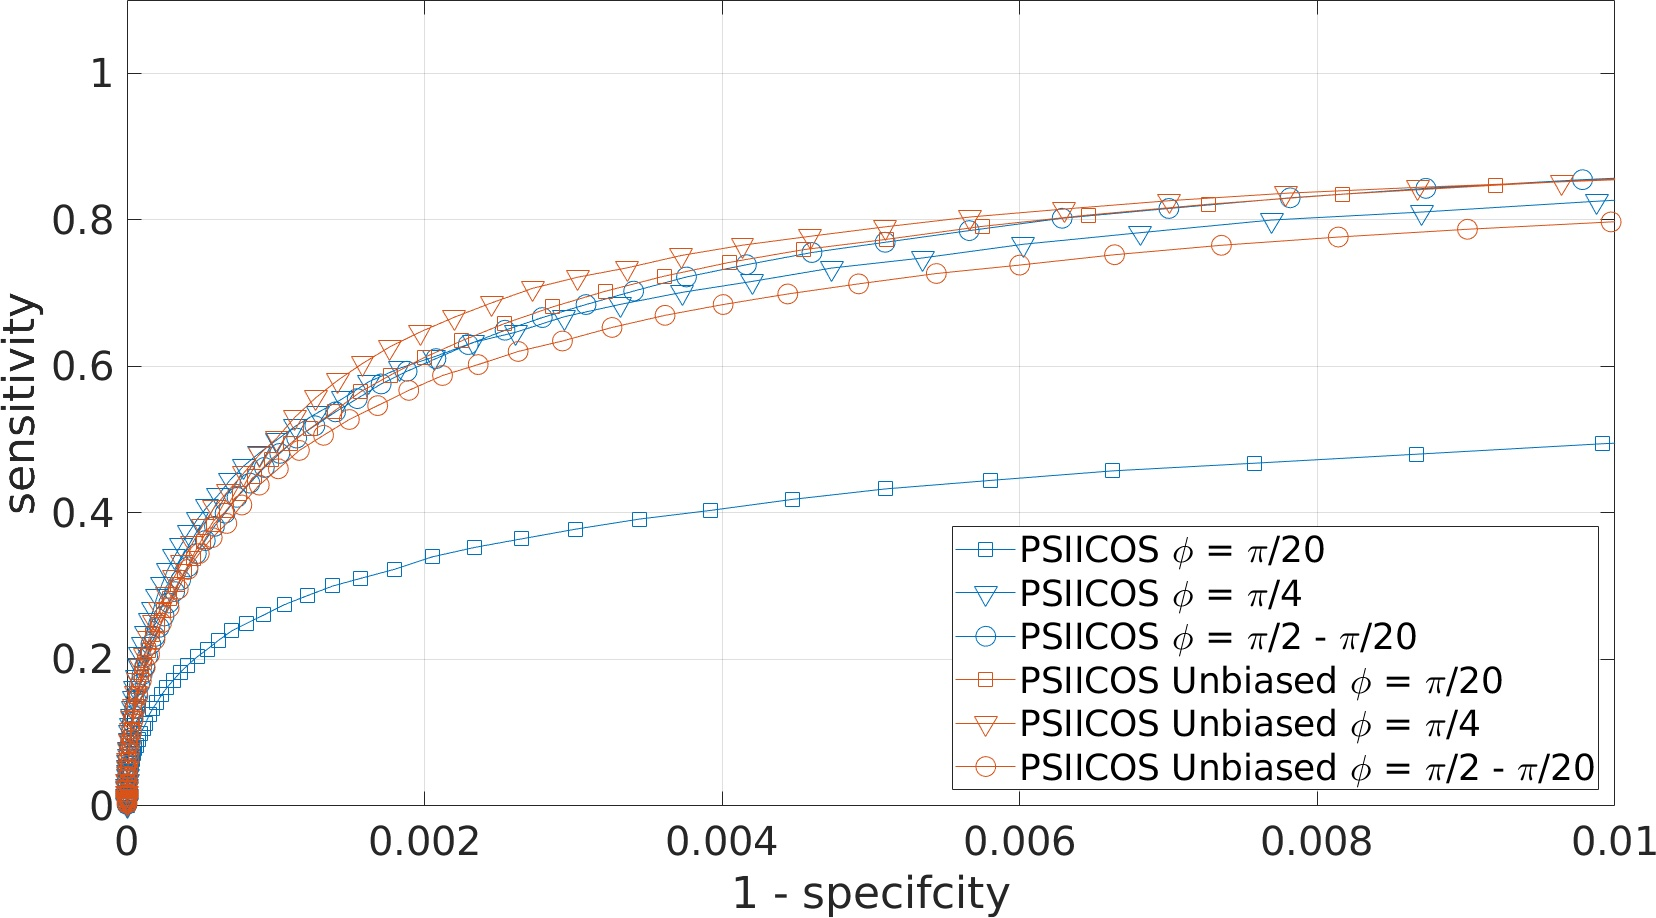
\includegraphics[width=0.99\linewidth]{../images/roc_3_ntw_snr_02.jpg}
        \caption{ROC, ОСШ=0.2}\label{fig:psiicos_vs_unbiased_3_ntw_d}
    \end{subfigure}
    \caption{Сравнение методов PSIICOS и PSIICOS Unbiased в задаче детекции трех сетей
        с фиксированными положениями источников и перекрывающимися временными профилями активации,
        усредненные по 10 повторениям.}\label{fig:psiicos_vs_unbiased_3_ntw}
\end{figure}

Результаты представлены на рис.~\ref{fig:psiicos_vs_unbiased_3_ntw}. Из этих графиков мы
вновь видим, что качество решений метода PSIICOS для малых фазовых задержек несколько проседает
по сравнению с PSIICOS Unbiased. При этом для фазовых сдвигов $\phi=\pi/4, \phi=\pi/2 - \pi/20$
качество решений PSIICOS по кривым оказывается несколько лучше, чем таковое для PSIICOS Unbiased.
Это объясняется способом построения соответствующих кривых и пространственной структурой сетей: метод
PSIICOS Unbiased для этой конкретной конфигурации склонен накапливать больше сетей вокруг одной из истинных
локаций, прежде чем переходить к остальным. Это приводит к выходу пучка отрезков за пределы
сферы, в которую должно попасть решение, что с точки зрения нашей процедуры является ложным срабатыванием,
но для реальных приложений не критично.

\section{Численное исследование метода нормализации кросс-спектральных коэффициентов в пространстве источников (PSIICOS Normalized).}\label{sec:psiicos_normalized_simulations}

В разделе~\ref{subsec:psiicos_normalized} мы обозначили проблему локализации методом PSIICOS,
которая заключается в том, что элементы кросс-спектра зависят не только от фазовой связности
источников, но и от их амплитуд, что не позволяет сделать однозначного вывода о наличии коннективности между парой источников.


\begin{figure}[htbp]
    \begin{subfigure}[t]{0.24\textwidth}
        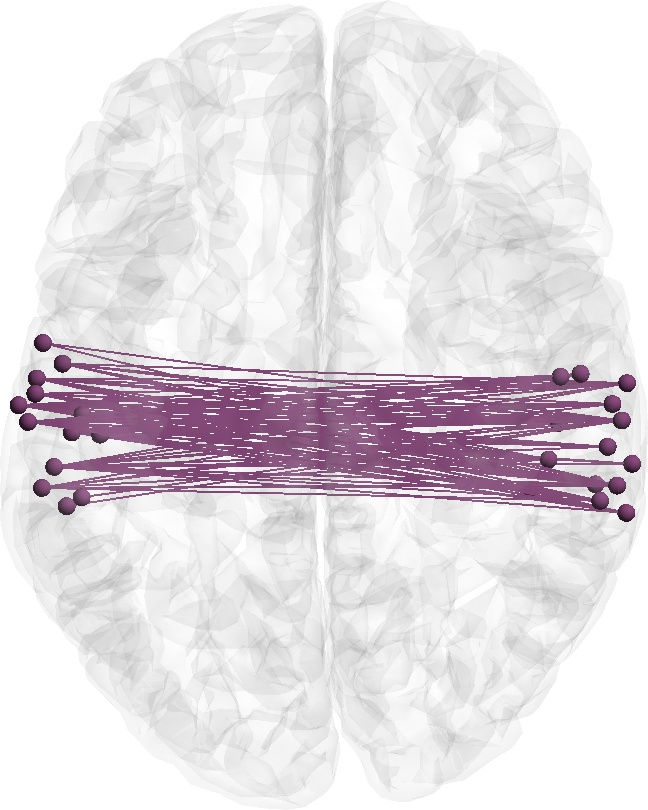
\includegraphics[width=0.99\textwidth]{../images/loreta_brain_jitter_01_snr_02_phase_lag_07854.jpg}
        \caption{$\alpha=0.1$, ОСШ=0.2}\label{fig:unbiased_1_ntw_a}
    \end{subfigure}
    \begin{subfigure}[t]{0.24\textwidth}
        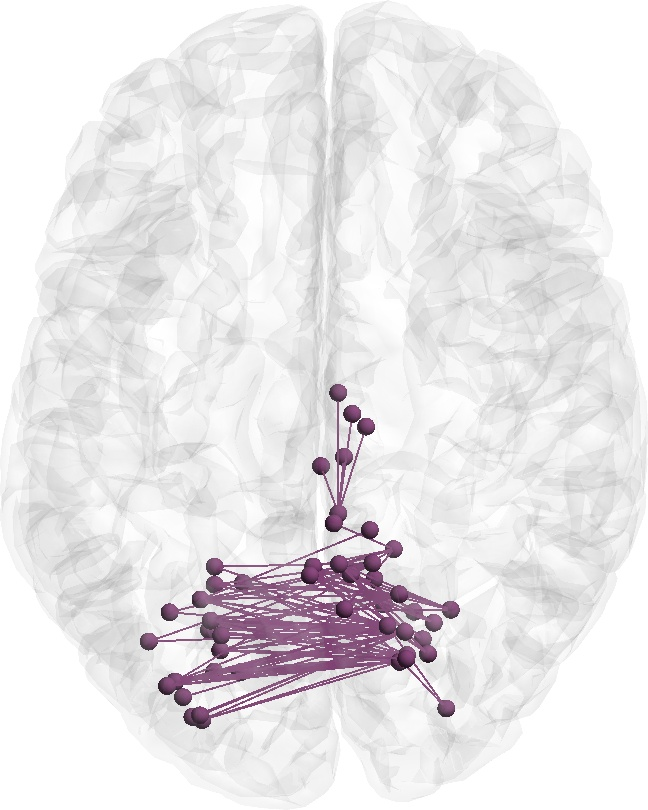
\includegraphics[width=0.99\linewidth]{../images/loreta_brain_jitter_2_snr_02_phase_lag_07854.jpg}
        \caption{$\alpha=2$, ОСШ=0.2}\label{fig:unbiased_1_ntw_b}
    \end{subfigure}
    \begin{subfigure}[t]{0.24\textwidth}
        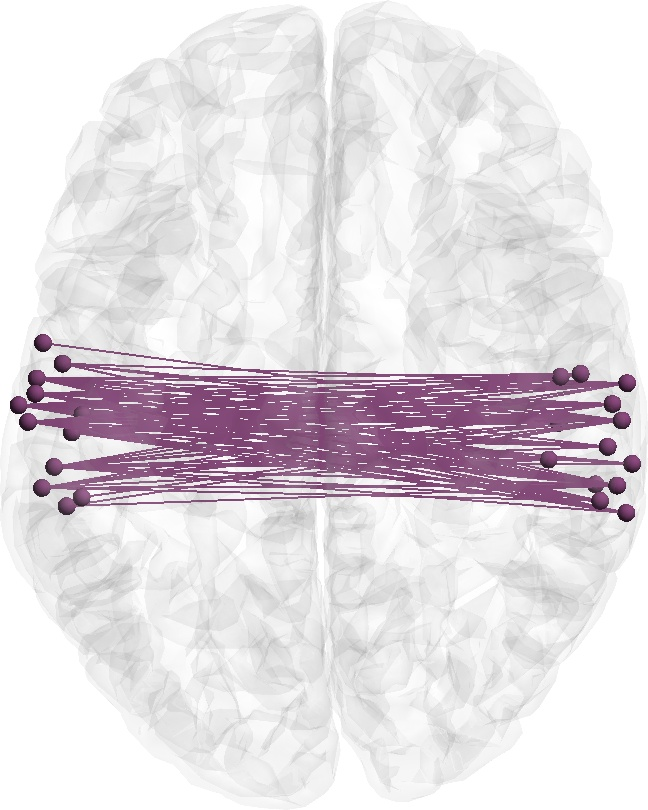
\includegraphics[width=0.99\textwidth]{../images/loreta_brain_jitter_01_snr_1_phase_lag_07854.jpg}
        \caption{$\alpha=0.1$, ОСШ=1}\label{fig:unbiased_1_ntw_c}
    \end{subfigure}
    \begin{subfigure}[t]{0.24\textwidth}
        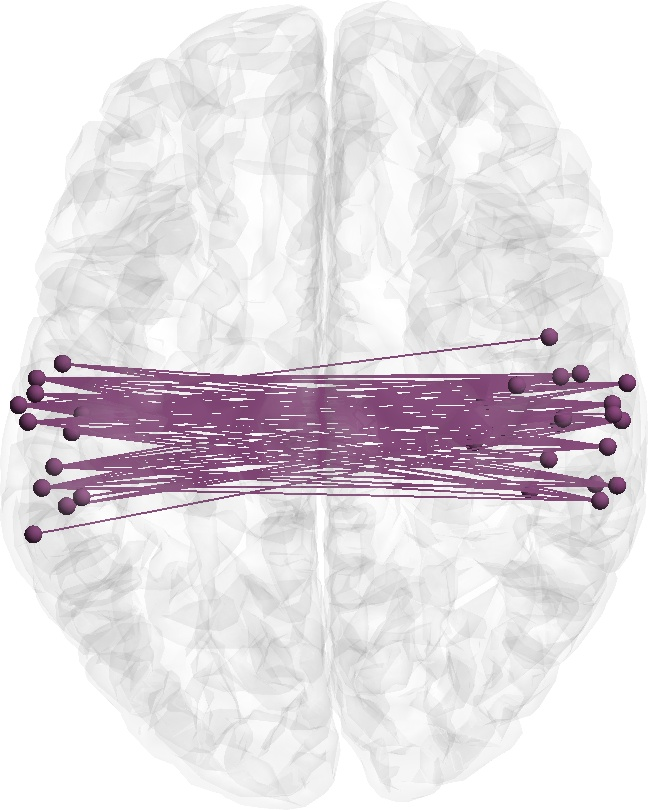
\includegraphics[width=0.99\linewidth]{../images/loreta_brain_jitter_2_snr_1_phase_lag_07854.jpg}
        \caption{$\alpha=2$, ОСШ=1}\label{fig:unbiased_1_ntw_d}
    \end{subfigure}
    \caption{Локализация сети с фиксированными положениями узлов методом PSIICOS Unbiased для
    фазового сдвига $\phi=\pi/4$ для высокого и низкого ОСШ (0.2 и 1) в
    случае сильной связности ($\alpha=0.1$) и отсутствия связности ($\alpha=2$)}\label{fig:unbiased_breaks_in_high_snr}
\end{figure}

На рис.~\ref{fig:unbiased_breaks_in_high_snr} мы проиллюстрировали этот эффект.
Для построения этого графика мы использовали симуляции, аналогичные описанным в
разделе~\ref{sec:three_ntw}, но на этот раз мы ограничились только одной
центральной сетью. На рис.~\ref{fig:unbiased_breaks_in_high_snr} мы показали
100 самых мощных сетей, полученных алгоритмом PSIICOS Unbiased для низкого и
высокого значения ОСШ при низком и высоком значении разброса фазы сети, $\alpha$.
Параметр $\alpha$ регулировал величину случайной добавки к постоянной
разности фаз для каждой сети. Чем ближе к нулю значение $\alpha$, тем сильнее
фазовая связность. Значение $\alpha=2$ соответствует полному отсутствию связности.

Из рис.~\ref{fig:unbiased_breaks_in_high_snr} видно, что алгоритм корректно находит
сети в случае высокой фазовой связности ($\alpha=0.1$, панели~\ref{fig:unbiased_1_ntw_a},~\ref{fig:unbiased_1_ntw_c}), однако при отсутствии фазовой связности ситуация не столь хороша.
В этом случае при низком ОСШ (панель~\ref{fig:unbiased_1_ntw_b}) алгоритм находит
шумовые сети, но так как выдаваемые им значения для сетей ненормированные, мы не можем
отбросить эти сети по одному прогону алгоритма. Тем не менее, эту проблему можно
решить, используя процедуру бутстрэпа и считая индекс воспроизводимости: для шумовых сетей
он будет низким, а для настоящих~--- высоким.

Хуже обстоит дело в случае отсутствия фазовой связности и высокого значения ОСШ (панель~\ref{fig:unbiased_1_ntw_d}). В при таких параметрах алгоритм находит ошибочно находит центральную сеть
из-за того, что мощность ее узлов выделяется на фоне окружающего шума, а также из-за
коррелированности их временных профилей активации. В этом случае процедура бутстрэпа
покажет воспроизводимую сеть, хотя в действительности фазовой связности нет.

В разделе~\ref{subsec:psiicos_normalized} мы предложили
модификацию метода PSIICOS, которая осуществляет нормализацию кросс-спектральных
коэффициентов с учетом наличия протечки сигнала. За счет нормализации мы можем справиться
с ложноположительными срабатываниями, аналогичными случаю~\ref{fig:unbiased_1_ntw_d}.

\begin{figure}[htbp]
    \begin{subfigure}[t]{0.5\textwidth}
        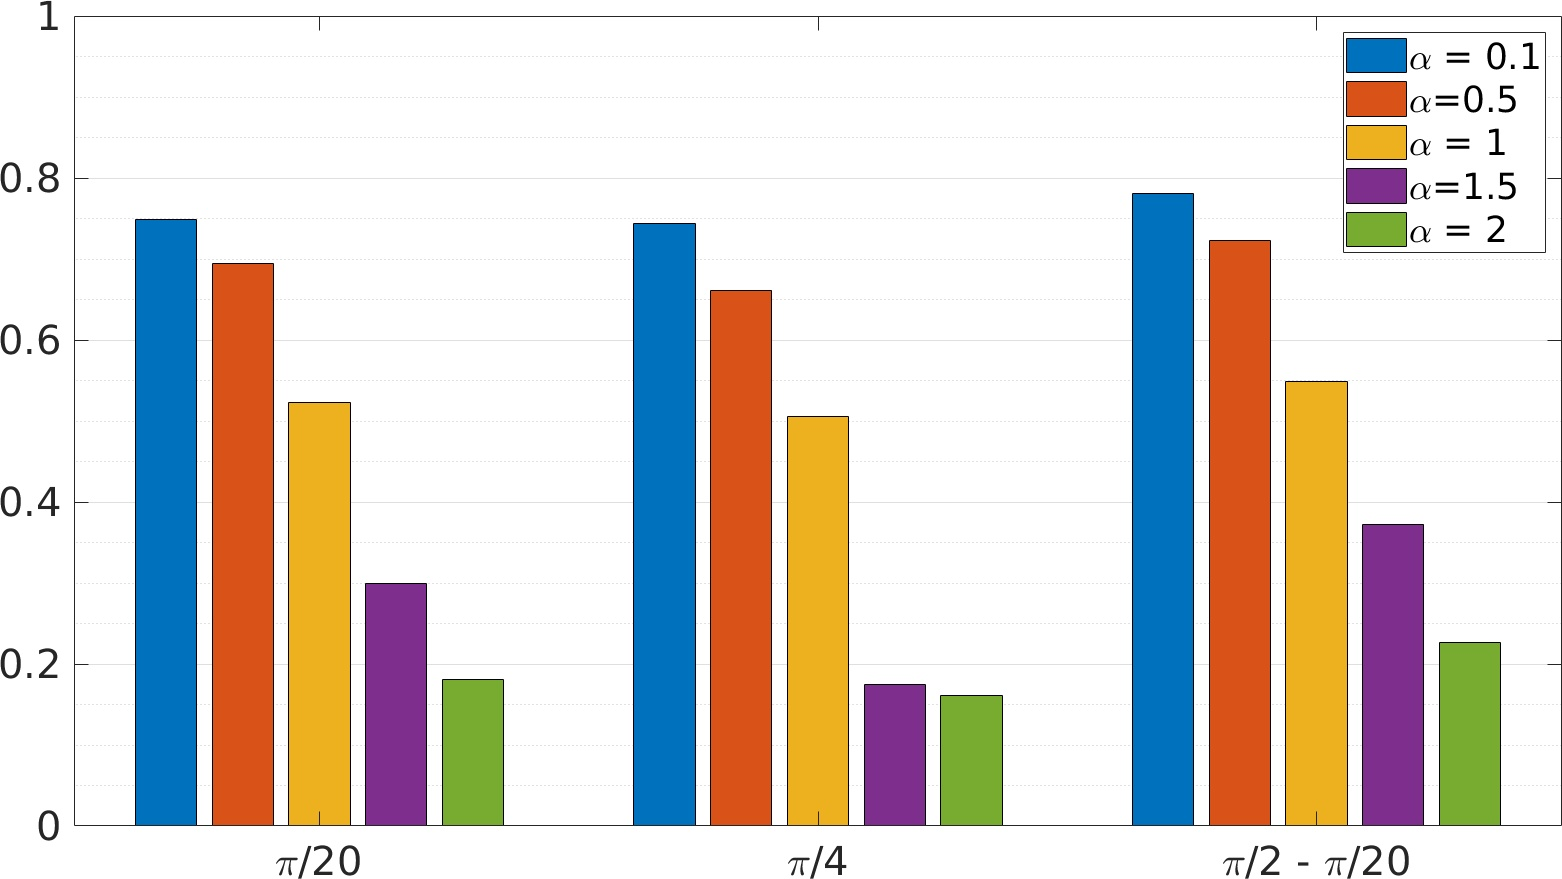
\includegraphics[width=0.99\textwidth]{../images/bars_snr_02.jpg}
        \caption{ОСШ=0.2}\label{fig:bars_a}
    \end{subfigure}
    \begin{subfigure}[t]{0.5\textwidth}
        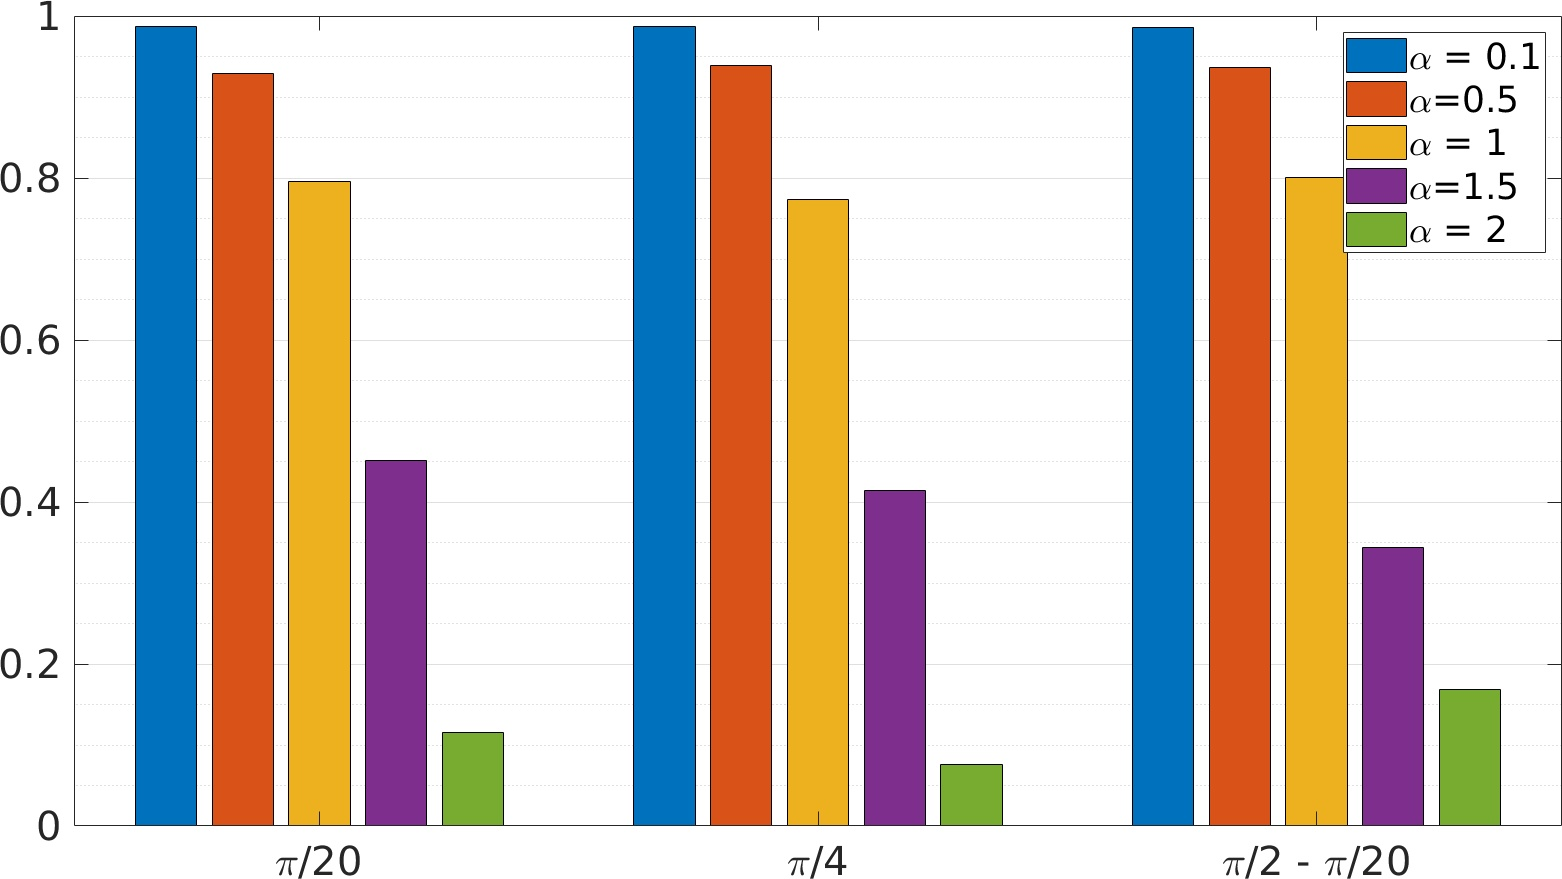
\includegraphics[width=0.99\linewidth]{../images/bars_snr_1.jpg}
        \caption{ОСШ=1}\label{fig:bars_b}
    \end{subfigure}
    \caption{Нормализованный индекс фазовой связности, полученный методом
    PSIICOS Normalized для одной симулированной сети в условиях высокого и низкого ОСШ
    в зависимости от индекса истинной фазовой связности $\alpha$ и значения
    фазовой задержки.}\label{fig:bars_normalized_index}
\end{figure}

Чтобы продемонстрировать это, мы симулировали данные для одной центральной сети
для набора индексов фазовой связности в диапазоне от 0.1 (сильная связность) до
2 (связность отсутствует) для низкого и высокого значения ОСШ (0.2 и 1 соответственно)
и для трех значений фазовых сдвигов ($\phi=\pi/20, \phi = \pi/4, \phi=\pi/2 - \pi/20$).
Для каждой комбинации параметров мы применяли метод PSIICOS Unbiased и отбирали
сети с максимальным абсолютным значением оцененного элемента кросс-спектра.
Для этой сети мы проводили нормализацию в соответствии с процедурой, описанной
в разд.~\ref{subsec:psiicos_normalized} и рисовали полученное значение на графике.
Результаты представлены на рис.~\ref{fig:bars_normalized_index}.

Из этого графика видно, что в случае, когда фазовая связность отсутствует
($\alpha=2$), полученные нормализованные значения не превосходят порога в 0.3.
При этом нормализованный индекс монотонно убывает с ростом параметра $\alpha$.

Вместе с тем отметим, что более высокое значение ОСШ позволяет получать более
высокие значения для нормализованного индекса для одинаковых значений $\alpha$
в случае, когда фазовая связность есть, оставляя индекс на том же уровне или
ниже, когда ее нет. Похожий эффект ослабления значений меры коннективности при
понижении ОСШ отмечали авторы метода wPLI,~\cite{wPLI}.

Индекс, полученный методом PSIICOS Normalized, теоретически может быть
использован и для локализации сетей, однако такая нормировка приводит к
появлению пространственной смещенности оценки (рассуждения аналогичны изложенным
в разд.~\ref{subsec:psiicos_normalization_and_spatial_bias}), поэтому для
использования на практике разумнее сначала локализовать потенциальные сети
одним из методов (PSIICOS Unbiased или GO-PSIICOS) и затем использовать
PSIICOS Normalized для удаления ложноположительных срабатываний из-за мощности.

\section{Демонстрация работы метода GO-PSIICOS на симуляционных данных.}

В этом разделе мы продемонстрировали работу метода GO-PSIICOS, который решает
задачу поиска сетей методом глобальной оптимизации и обладает свойством разреженности
решений по пространству, что позволяет подавить ``призрачные взаимодействия'' в
решении.


\begin{figure}[htbp]
    \begin{subfigure}[t]{0.6\textwidth}
        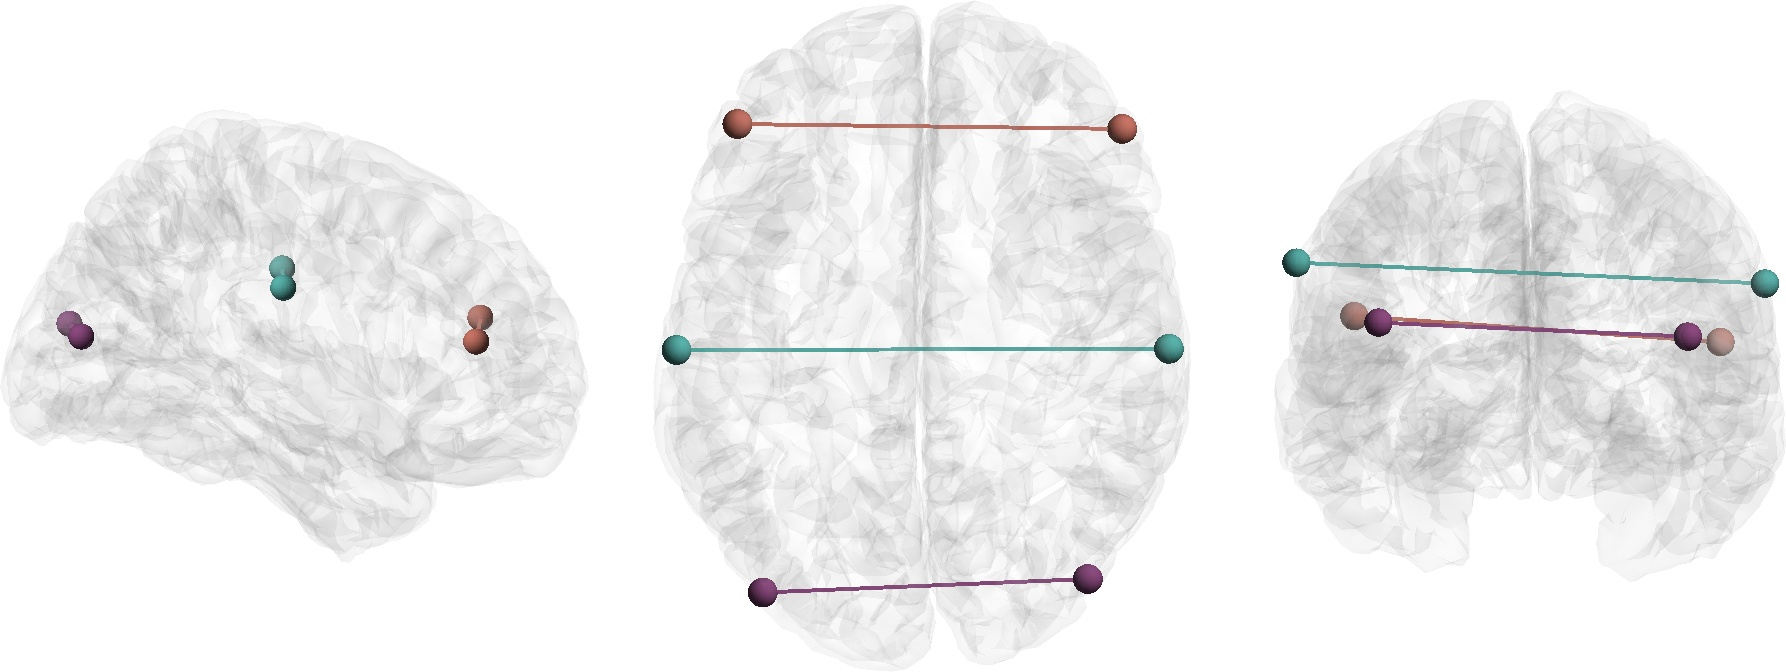
\includegraphics[width=0.99\textwidth]{../images/networks_gopsiicos.jpg}
        \caption{Восстановленные сети, $\phi=\pi/20$}\label{fig:gopsiicos_a}
    \end{subfigure}
    \begin{subfigure}[t]{0.4\textwidth}
        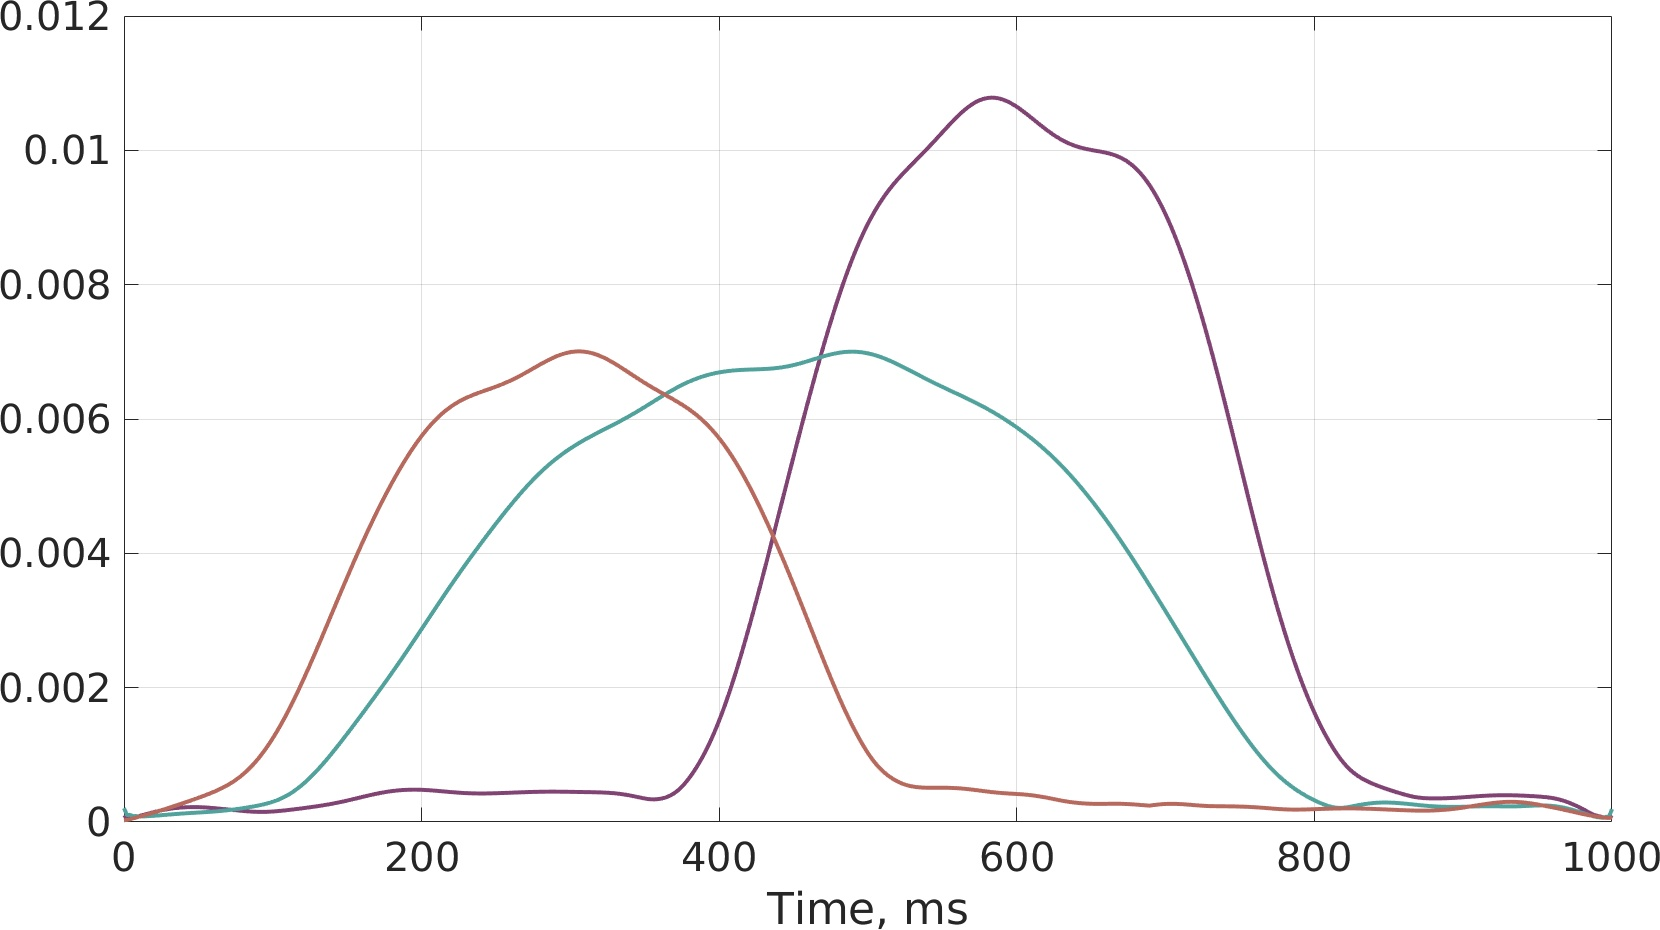
\includegraphics[width=0.99\linewidth]{../images/timeseries_gopsiicos.jpg}
        \caption{Восстановленные профили активации $\phi=\pi/20$}\label{fig:gopsiicos_b}
    \end{subfigure}
    \begin{subfigure}[t]{0.6\textwidth}
        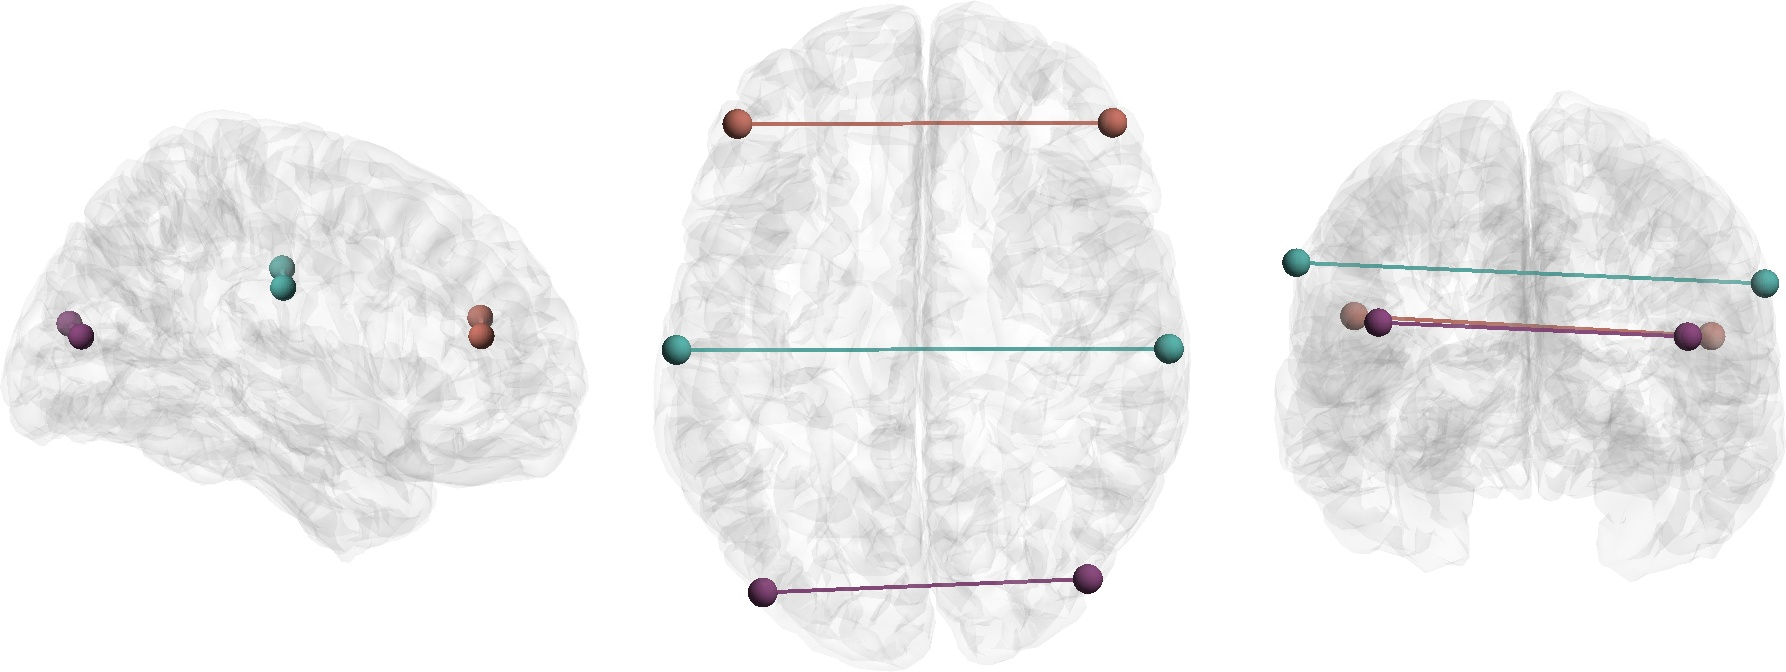
\includegraphics[width=0.99\textwidth]{../images/networks_gopsiicos_pi4.jpg}
        \caption{Восстановленные сети, $\phi=\pi/4$}\label{fig:gopsiicos_c}
    \end{subfigure}
    \begin{subfigure}[t]{0.4\textwidth}
        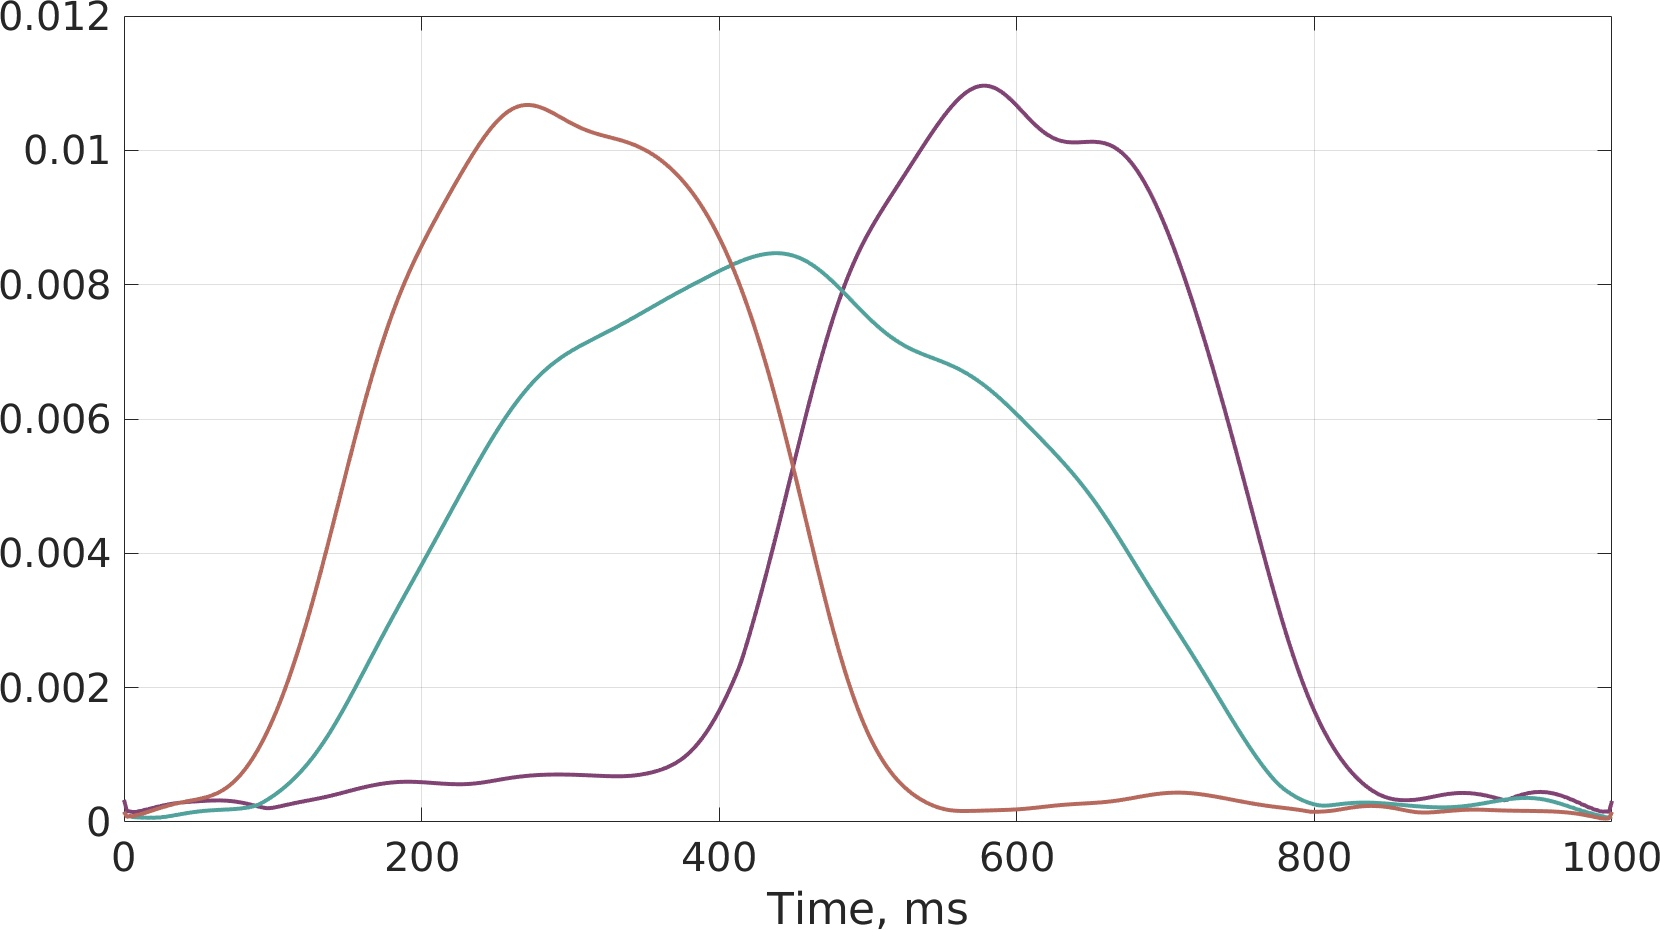
\includegraphics[width=0.99\linewidth]{../images/timeseries_gopsiicos_pi4.jpg}
        \caption{Восстановленные профили активации $\phi=\pi/4$}\label{fig:gopsiicos_d}
    \end{subfigure}
    \begin{subfigure}[t]{0.6\textwidth}
        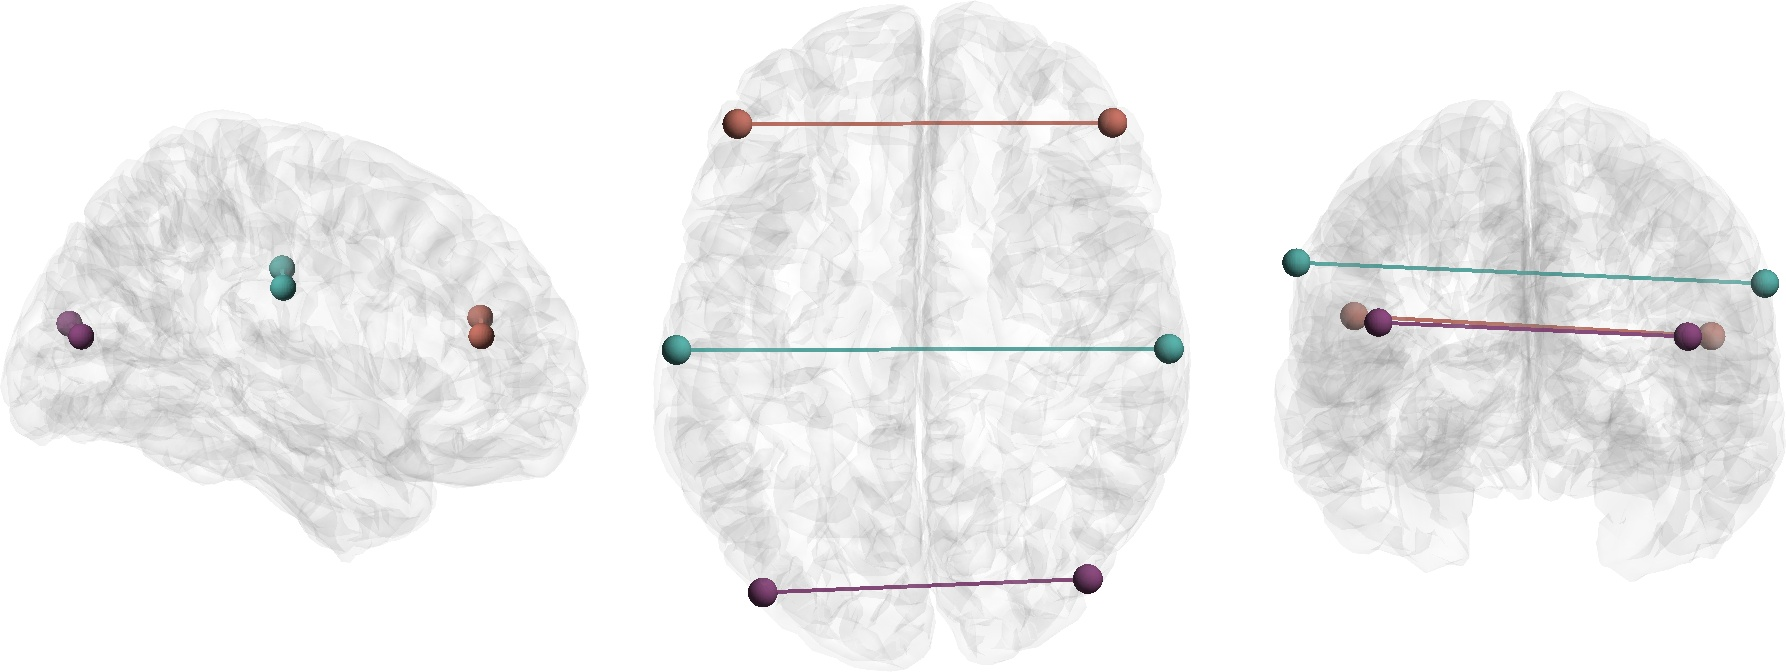
\includegraphics[width=0.99\textwidth]{../images/networks_gopsiicos_pi2pi20.jpg}
        \caption{Восстановленные сети, $\phi=\pi/2-\pi/20$}\label{fig:gopsiicos_e}
    \end{subfigure}
    \begin{subfigure}[t]{0.4\textwidth}
        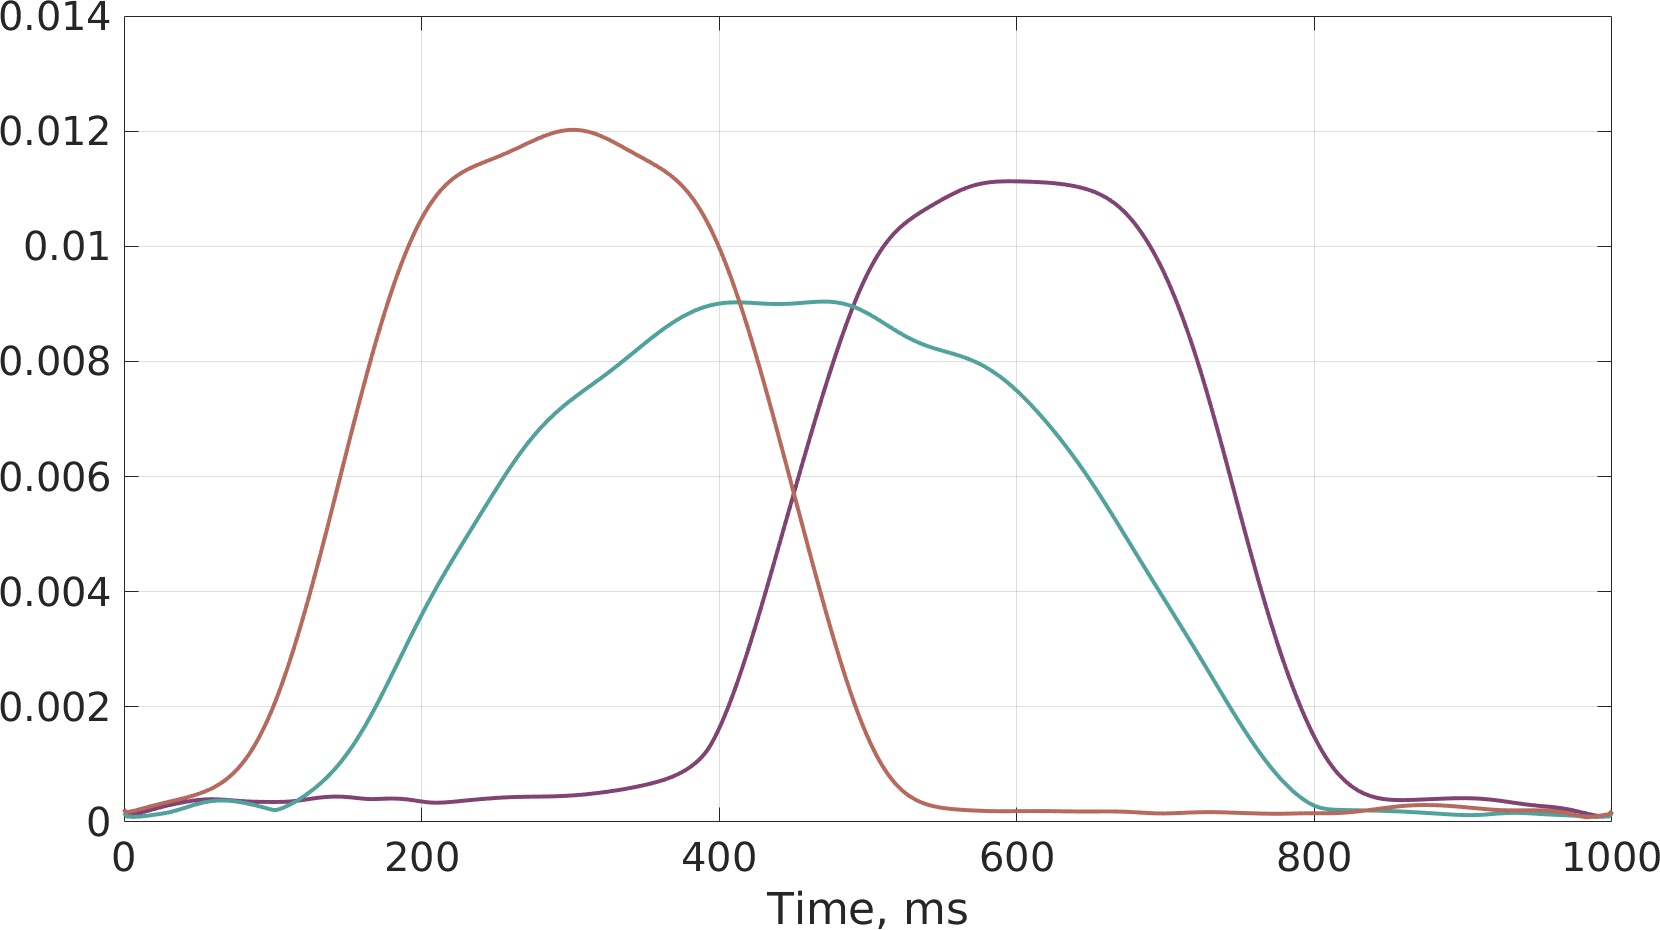
\includegraphics[width=0.99\linewidth]{../images/timeseries_gopsiicos_pi2pi20.jpg}
        \caption{Восстановленные профили активации $\phi=\pi/2-\pi/20$}\label{fig:gopsiicos_f}
    \end{subfigure}
    \caption{Применение метода GO-PSIICOS к задаче детекции трех сетей с перекрывающимися профилями активности для ОСШ=0.5 и фазовых сдвигов $\phi=\pi/20, \phi=\pi/4, \phi=\pi/2-\pi/20$.}\label{fig:gopsiicos}
    Цвета сетей на панели~\ref{fig:gopsiicos_a} соответствуют цветам восстановленных
    профилей на панели~\ref{fig:gopsiicos_b}.
\end{figure}

Для демонстрации работы метода мы использовали симуляции с тремя
сетями с перекрывающимися профилями активности, описанные в разд.~\ref{sec:three_ntw}.
Результаты работы метода для ОСШ=0.5 представлены на рис.~\ref{fig:gopsiicos}.

Как видно на графике, алгоритм справился с нахождением всех трех сетей и достаточно
точно восстановил их временные профили.
